% arguelles v2.3.0
% author: Michele Piazzai
% contact: michele.piazzai@uc3m.es
% license: MIT

% Copied from GitHub: https://github.com/piazzai/arguelles

\documentclass[aspectratio=169,compress,12pt,dvipsnames]{beamer}

\usetheme{Arguelles}

%%%%%%%%%%%%%%%%%%%%%%%%%%%%%%%%%%%%%%%%%%%%%%%%%
%%%%%                                       %%%%%
%%%%%     LIST OF USEFUL LaTeX PACKAGES     %%%%%
%%%%%                                       %%%%%
%%%%%%%%%%%%%%%%%%%%%%%%%%%%%%%%%%%%%%%%%%%%%%%%%

% ---
% Character encoding
% ---
\usepackage[T1]{fontenc}
\usepackage[utf8]{inputenc}
\usepackage[]{fontawesome5}

% ---
% Language related packages
% ---
\usepackage[english]{babel}
\usepackage[abbreviations,british]{foreign}

% ---
% Bibliography-related
% ---
% \usepackage[numbers, sort&compress]{natbib}
%
% ---
% Colours
% ---
\usepackage[]{color}
\usepackage[]{xcolor}

% ---
% Figures
% ---
\usepackage[]{graphicx}
\usepackage[]{subfigure}

% ---
% Mathematics
% ---
\usepackage[]{mathtools}
\usepackage[]{amssymb, amsmath, amsfonts}
\usepackage[]{yhmath}
\usepackage[]{stmaryrd}
\usepackage[]{nicefrac}
\usepackage[]{algpseudocode}

% ---
% Physics
% ---
\usepackage[]{siunitx}
\usepackage[]{physics}

% ---
% Tikz-related
% ---
\usepackage{listofitems}
\usepackage[]{tikz, ifthen}
\usetikzlibrary{arrows}
\usetikzlibrary{shapes}
\usetikzlibrary{positioning}
\usetikzlibrary{tikzmark}
\usetikzlibrary{patterns}
\usetikzlibrary{backgrounds}
\usetikzlibrary{angles}
\usetikzlibrary{quotes}
\tikzset{>=latex} % for LaTeX arrow head
\colorlet{veccol}{green!70!black}
\colorlet{vcol}{green!70!black}
\colorlet{xcol}{blue!85!black}
\colorlet{projcol}{xcol!60}
\colorlet{unitcol}{xcol!60!black!85}

\colorlet{myblue}{blue!70!black}
\colorlet{myred}{red!90!black}
\colorlet{mypurple}{blue!50!red!80!black!80}
\colorlet{mygreen}{green!60!black}
\colorlet{myorange}{orange!70!red!60!black}
\colorlet{mydarkred}{red!30!black}
\colorlet{mydarkblue}{blue!40!black}
\colorlet{mydarkgreen}{green!30!black}

\tikzstyle{vector}=[->,very thick,xcol]
\tikzset{
  >=latex, % for default LaTeX arrow head
  node/.style={thick,circle,draw=myblue,minimum size=22,inner sep=0.5,outer sep=0.6},
  node in/.style={node,green!20!black,draw=mygreen!30!black,fill=mygreen!25},
  node hidden/.style={node,blue!20!black,draw=myblue!30!black,fill=myblue!20},
  node convol/.style={node,orange!20!black,draw=myorange!30!black,fill=myorange!20},
  node out/.style={node,red!20!black,draw=myred!30!black,fill=myred!20},
  connect/.style={thick,mydarkblue}, %,line cap=round
  connect arrow/.style={-{Latex[length=4,width=3.5]},thick,mydarkblue,shorten <=0.5,shorten >=1},
  node 1/.style={node in}, % node styles, numbered for easy mapping with \nstyle
  node 2/.style={node hidden},
  node 3/.style={node out}
}
\def\nstyle{int(\lay<\Nnodlen?min(2,\lay):3)} % map layer number onto 1, 2, or 3

\newcommand{\stencilpt}[4][]{\node[circle,fill=blue!60,draw=black,scale=0.5,label={below:#4},#1] at (#2) (#3) {}}

\usepackage[]{pgfplots}
\usepgfplotslibrary{fillbetween}

\usepackage[]{tikz-network}

% ---
% Code
% ---
\usepackage{listings}

\definecolor{codegreen}{rgb}{0,0.6,0}
\definecolor{codegray}{rgb}{0.5,0.5,0.5}
\definecolor{codepurple}{rgb}{0.58,0,0.82}
\definecolor{backcolour}{rgb}{0.95,0.95,0.92}

\lstdefinestyle{mystyle}{
  backgroundcolor=\color{backcolour},   
  commentstyle=\color{codegreen},
  keywordstyle=\color{magenta},
  numberstyle=\tiny\color{codegray},
  stringstyle=\color{codepurple},
  basicstyle=\ttfamily\footnotesize,
  breakatwhitespace=false,         
  breaklines=true,                 
  captionpos=b,                    
  keepspaces=true,                 
  % numbers=left,                    
  numbersep=5pt,                  
  showspaces=false,                
  showstringspaces=false,
  showtabs=false,                  
  tabsize=2
}

\lstset{style=mystyle}

% ---
% Miscellaneous
% ---
\usepackage[]{lipsum}
\usepackage[]{xparse}
\usepackage{multicol}
\usepackage{pifont}

%%%%%%%%%%%%%%%%%%%%%%%%%%%%%%%%%%%%%%%%%%%%%%%
%%%%%                                     %%%%%
%%%%%     LIST OF COMMANDS AND MACROS     %%%%%
%%%%%                                     %%%%%
%%%%%%%%%%%%%%%%%%%%%%%%%%%%%%%%%%%%%%%%%%%%%%%

% ---
% Annotating equations using Tikz
% ---
\newcommand{\highlight}[2]{\colorbox{#1!17}{\ensuremath{\displaystyle #2}}}
\newcommand{\highlightdark}[2]{\colorbox{#1!47}{\ensuremath{\displaystyle #2}}}

% ---
% Mathematics
% ---

% Simple macros
\renewcommand{\det}[1]{\text{det}\left( #1 \right)}
\renewcommand{\trace}[1]{\text{Tr}\left( #1 \right)}
\newcommand{\Span}[1]{\text{Span}\left( #1 \right)}
\newcommand{\conj}[1]{\ensuremath{#1^*}}


% Algebra
\newcommand{\e}{\ensuremath{\mathrm{e}}}

\newcommand{\R}{\ensuremath{\mathbb{R}}}
\newcommand{\C}{\ensuremath{\mathbb{C}}}
\newcommand{\K}{\ensuremath{\mathbb{K}}}

\newcommand{\innerprod}[2]{\ensuremath{\left\langle #1 \vert #2 \right\rangle}}

% Linear algebra
\newcommand{\allones}{\ensuremath{\mathbf{1}}}
\newcommand{\allzeros}{\ensuremath{\mathbf{0}}}
\newcommand{\Gram}[1]{\ensuremath{\mathbf{#1}^* \mathbf{#1}}}
\newcommand{\inv}[1]{\ensuremath{\mathbf{#1}^{-1}}}
\newcommand{\pinv}[1]{\ensuremath{\mathbf{#1}^{\dagger}}}
\newcommand{\svd}[1]{\ensuremath{\mathbf{U}_{#1} \boldsymbol{\Sigma}_{#1} \mathbf{V}^T_{#1}}}

% Probability and statistics
\newcommand{\E}[1]{\ensuremath{\mathbb{E} \left[ #1 \right]}}
\newcommand{\covmat}[1]{\ensuremath{\mathbf{C}_{\mathbf{#1}}}}

% Optimization problems
\DeclareMathOperator*{\minimize}{minimize~}
\DeclareMathOperator*{\argmin}{argmin~}

\DeclareMathOperator*{\maximize}{maximize~}
\DeclareMathOperator*{\argmax}{argmax~}

\DeclareMathOperator{\subto}{subject~to~}

% Column and row vectors.
\ExplSyntaxOn
\NewDocumentCommand{\colvec}{O{1}m}
{
  \scalebox{#1}{$\generalvec{#2}{\\}$}
}
\NewDocumentCommand{\rowvec}{O{1}m}
{
  \scalebox{#1}{$\generalvec{#2}{&}$}
}
\NewDocumentCommand{\generalvec}{mm}
{
  \clist_set:Nn \l_tmpa_clist { #1 }
  %\renewcommand{\arraystretch}{.8}
  \begin{bmatrix}
    \clist_use:Nn \l_tmpa_clist { #2 }
  \end{bmatrix}
}
\ExplSyntaxOff
\usefonttheme{professionalfonts}

\graphicspath{{./imgs/}}

\title{Apprentissage statistique pour la physique}
\subtitle{Physics Informed Neural Networks}
\event{}
\date{}
\author{Jean-Christophe Loiseau}
\institute{Arts \& Métiers}
\email{jean-christophe.loiseau@ensam.eu}
\homepage{loiseaujc.github.io}
\github{loiseaujc}

\begin{document}

\frame[plain]{\titlepage}

%%%%%%%%%%%%%%%%%%%%%%%%%%%%%%%%
%%%%%     INTRODUCTION     %%%%%
%%%%%%%%%%%%%%%%%%%%%%%%%%%%%%%%

\begin{frame}[plain]{Qui suis-je ?}
  \vfill
  \begin{minipage}{.28\textwidth}
    \centering
    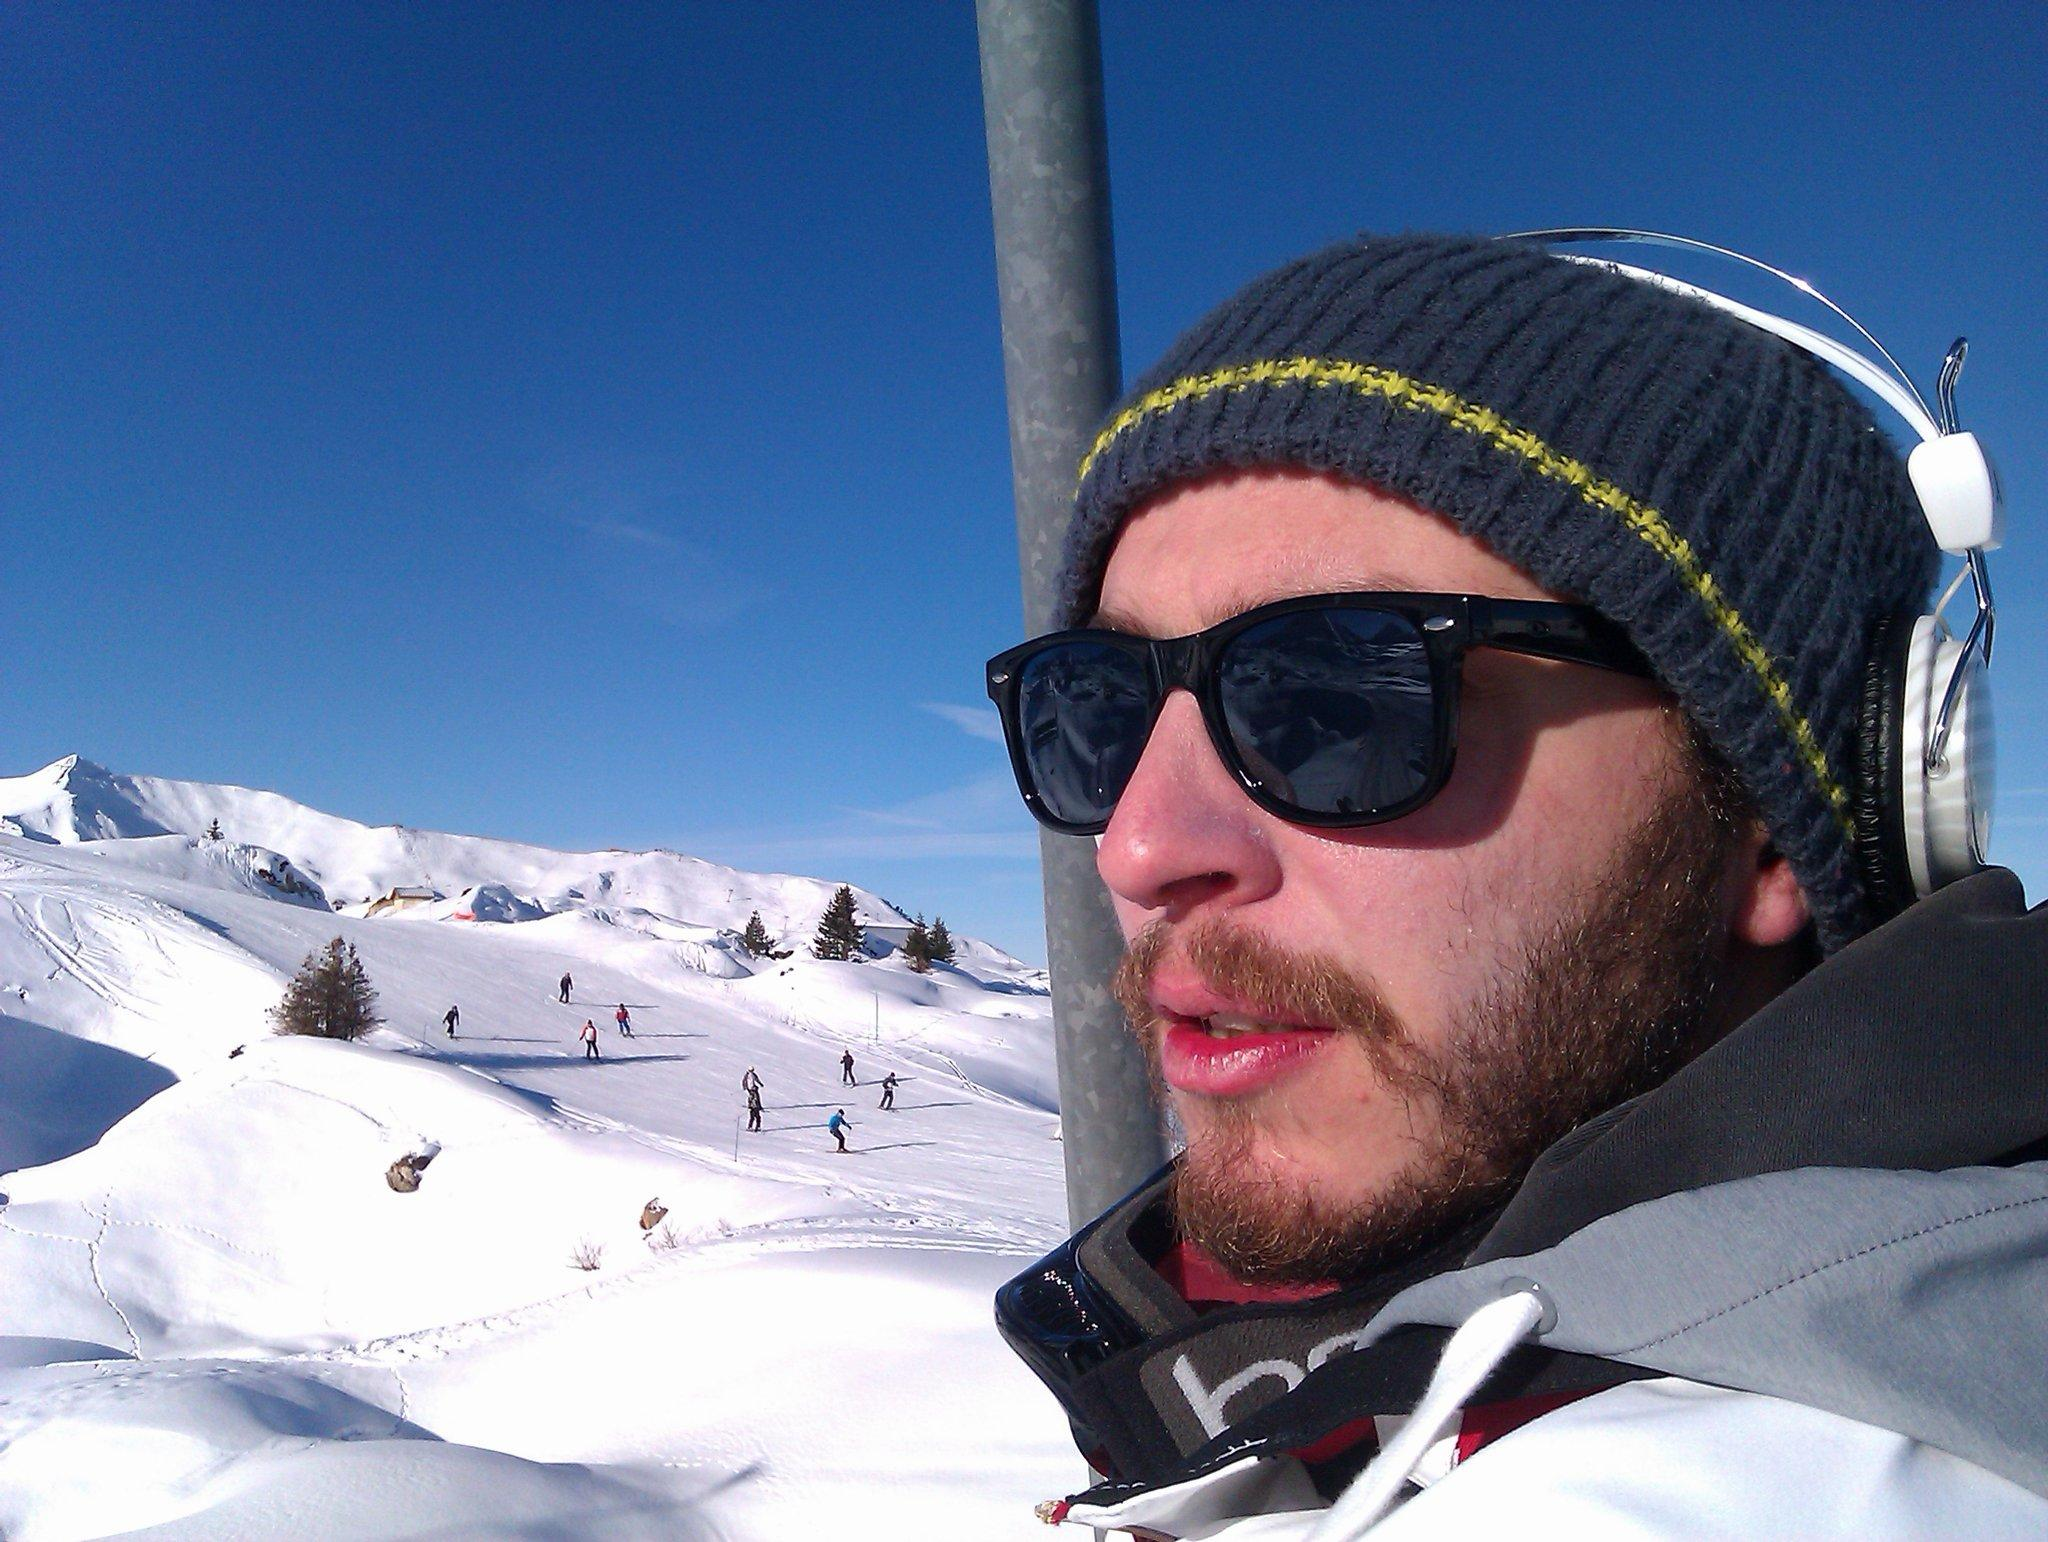
\includegraphics[width=\textwidth]{myself.jpg}
  \end{minipage}%
  \hfill
  \begin{minipage}{.68\textwidth}
    \begin{itemize}
      \item Maître de Conférences à l'Ecole Nationale Supérieure d'Arts et Métiers, Paris.
        \par
      \item Recherche orientée autour de trois axes principaux:
        \begin{itemize}
          \item Transition à la turbulence.
          \item Modélisation réduite et identification de systèmes.
          \item Contrôle et Estimation.
        \end{itemize}
    \end{itemize}
  \end{minipage}
  \vfill
\end{frame}

\begin{frame}[standout, plain]
  \vfill
  \centering
  {\usebeamerfont{title}Apprentissage statistique pour et par la Physique}
  \vfill
\end{frame}

\begin{frame}[plain]{Déroulement du cours}
  \vfill
  \begin{minipage}{.68\textwidth}
    \underline{\textbf{Cours 1} --  Réseaux de neurones informés par la Physique}
    %
    \par\bigskip
    %
    \begin{tabular}{cl}
      \faClock          & Lundi 6 janvier, 10h15-12h15  \\
      \\
      \faClipboardList  & Résolution d'une EDP à l'aide d'un PINN \\
      & PINNS et problèmes inverses \\
      & Limites des PINNs \\
      \\
      \faPython         & \url{???}
    \end{tabular}
    %
    \par\medskip
    %
  \end{minipage}%
  \hfill
  \begin{minipage}{.28\textwidth}
    \centering
    \scalebox{4}{\faBook}
  \end{minipage}
  \vfill
\end{frame}

\begin{frame}[plain]{Déroulement du cours}
  \vfill
  \begin{minipage}{.68\textwidth}
    \underline{\textbf{TP/TD} --  Physics-Informed Neural Networks}
    %
    \par\bigskip
    %
    \begin{tabular}{cl}
      \faClock          & Lundi 6 janvier, 14h00-17h00  \\
      \\
      \faClipboardList  & Résolution de l'équation de Burgers \\
      & Trucs et Astuces \\
      \\
      \faPython         & \url{???}
    \end{tabular}
    %
    \par\medskip
    %
  \end{minipage}%
  \hfill
  \begin{minipage}{.28\textwidth}
    \centering
    \scalebox{4}{\faBook}
  \end{minipage}
  \vfill
\end{frame}

\begin{frame}[plain]{Déroulement du cours}
  \vfill
  \begin{minipage}{.68\textwidth}
    \underline{\textbf{Cours 2} --  Identification de systèmes non-linéaires}
    %
    \par\bigskip
    %
    \begin{tabular}{cl}
      \faClock          & Mardi 7 janvier, 09h30-10h30  \\
      \\
      \faClipboardList  & Le principe de parcimonie \\
      & \emph{Sparse Identification of Nonlinear Dynamics}  \\
      & Illustrations \\
      \\
      \faPython         & \url{???}
    \end{tabular}
    %
    \par\medskip
    %
  \end{minipage}%
  \hfill
  \begin{minipage}{.28\textwidth}
    \centering
    \scalebox{4}{\faBook}
  \end{minipage}
  \vfill
\end{frame}

\begin{frame}[plain]{Déroulement du cours}
  \vfill
  \begin{minipage}{.68\textwidth}
    \underline{\textbf{TP/TD} --  SINDy}
    %
    \par\bigskip
    %
    \begin{tabular}{cl}
      \faClock          & Mardi 7 janvier, 10h30-12h30  \\
      \\
      \faClipboardList  & Optimisation convexe \\
      &  \texttt{pySINDy}\\
      \\
      \faPython         & \url{???}
    \end{tabular}
    %
    \par\medskip
    %
  \end{minipage}%
  \hfill
  \begin{minipage}{.28\textwidth}
    \centering
    \scalebox{4}{\faBook}
  \end{minipage}
  \vfill
\end{frame}

\begin{frame}[standout, plain]
  \vfill
  {\usebeamerfont{title} Physics Informed Neural Networks}

  {\usebeamerfont{subtitle} PINNs}
  \vfill
\end{frame}

\section{Introduction}

\begin{frame}
  \vfill
  \begin{minipage}{.68\textwidth}
    \begin{itemize}
      \item Proposed by Raissi, Perdikaris et Karniadakis in 2017 for solving PDE.
    \end{itemize}
    %
    \bigskip
    %
    \textbf{Idea}  \hspace{1em}  Leverage the universal approximation capabilities of neural nets to represent the solution to a PDE.
  \end{minipage}%
  \hfill
  \begin{minipage}{.28\textwidth}
    \centering
    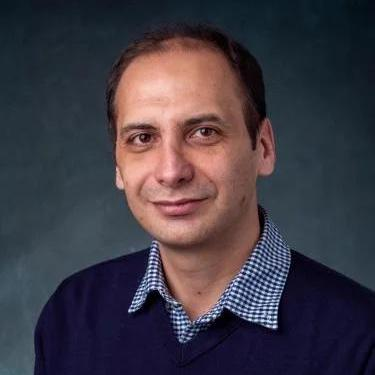
\includegraphics[width=\textwidth]{mazar_raissi.jpeg}
    \par
    {\tiny
    Maziar Raissi
    }
  \end{minipage}
  \vfill
\end{frame}

\section{Kalman smoothing}

\begin{frame}[standout, plain]
  \vfill
  {\usebeamerfont{title} Kalman smoothing}

  {\usebeamerfont{subtitle} A (rapid) detour through convex optimization}
  \vfill
\end{frame}

\begin{frame}
  \vfill
  \begin{minipage}{.28\textwidth}
    \[
      \begin{aligned}
        \vb{x}_{t+1}  & = \vb{Ax}_t + \vb{w}_t \\
        \vb{y}_t      & = \vb{Cx}_t + \vb{v}_t
      \end{aligned}
    \]
  \end{minipage}%
  \hfill
  \begin{minipage}{.68\textwidth}
    \centering
    \begin{tabular}{lc}
      \textbf{State vector} & $\vb{x} \in \R^n$ \\
      \textbf{Transition matrix}  & $\vb{A} \in \R^{n \times n}$, $\rho(\vb{A}) < 1$  \\
      \textbf{Measurement operator} & $\vb{C} \in \R^{q \times n}$  \\
      \textbf{Process noise}  & $\vb{w}_t \sim \mathcal{N}(\vb{0}, \vb{W})$ \\
      \textbf{Sensor noise}   & $\vb{v}_t \sim \mathcal{N}(\vb{0}, \vb{V})$
    \end{tabular}
  \end{minipage}
  \vfill
\end{frame}

\begin{frame}
  \vfill
  Given $\vb{A}$, $\vb{C}$ and the sequence $\left\{ \vb{y}_t \right\}_{t=0, \cdots, T}$, can we uniquely determine the most likely state sequence $\left\{ \vb{x}_t \right\}_{t=0, \cdots, T}$ ?

  \vfill

  \begin{minipage}{.28\textwidth}
    \centering
    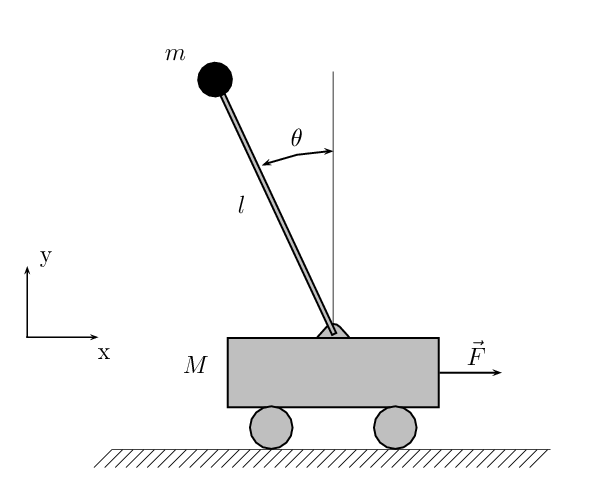
\includegraphics[width=\textwidth]{Cart-pendulum.png}
  \end{minipage}%
  \hfill
  \begin{minipage}{.68\textwidth}
    \centering
    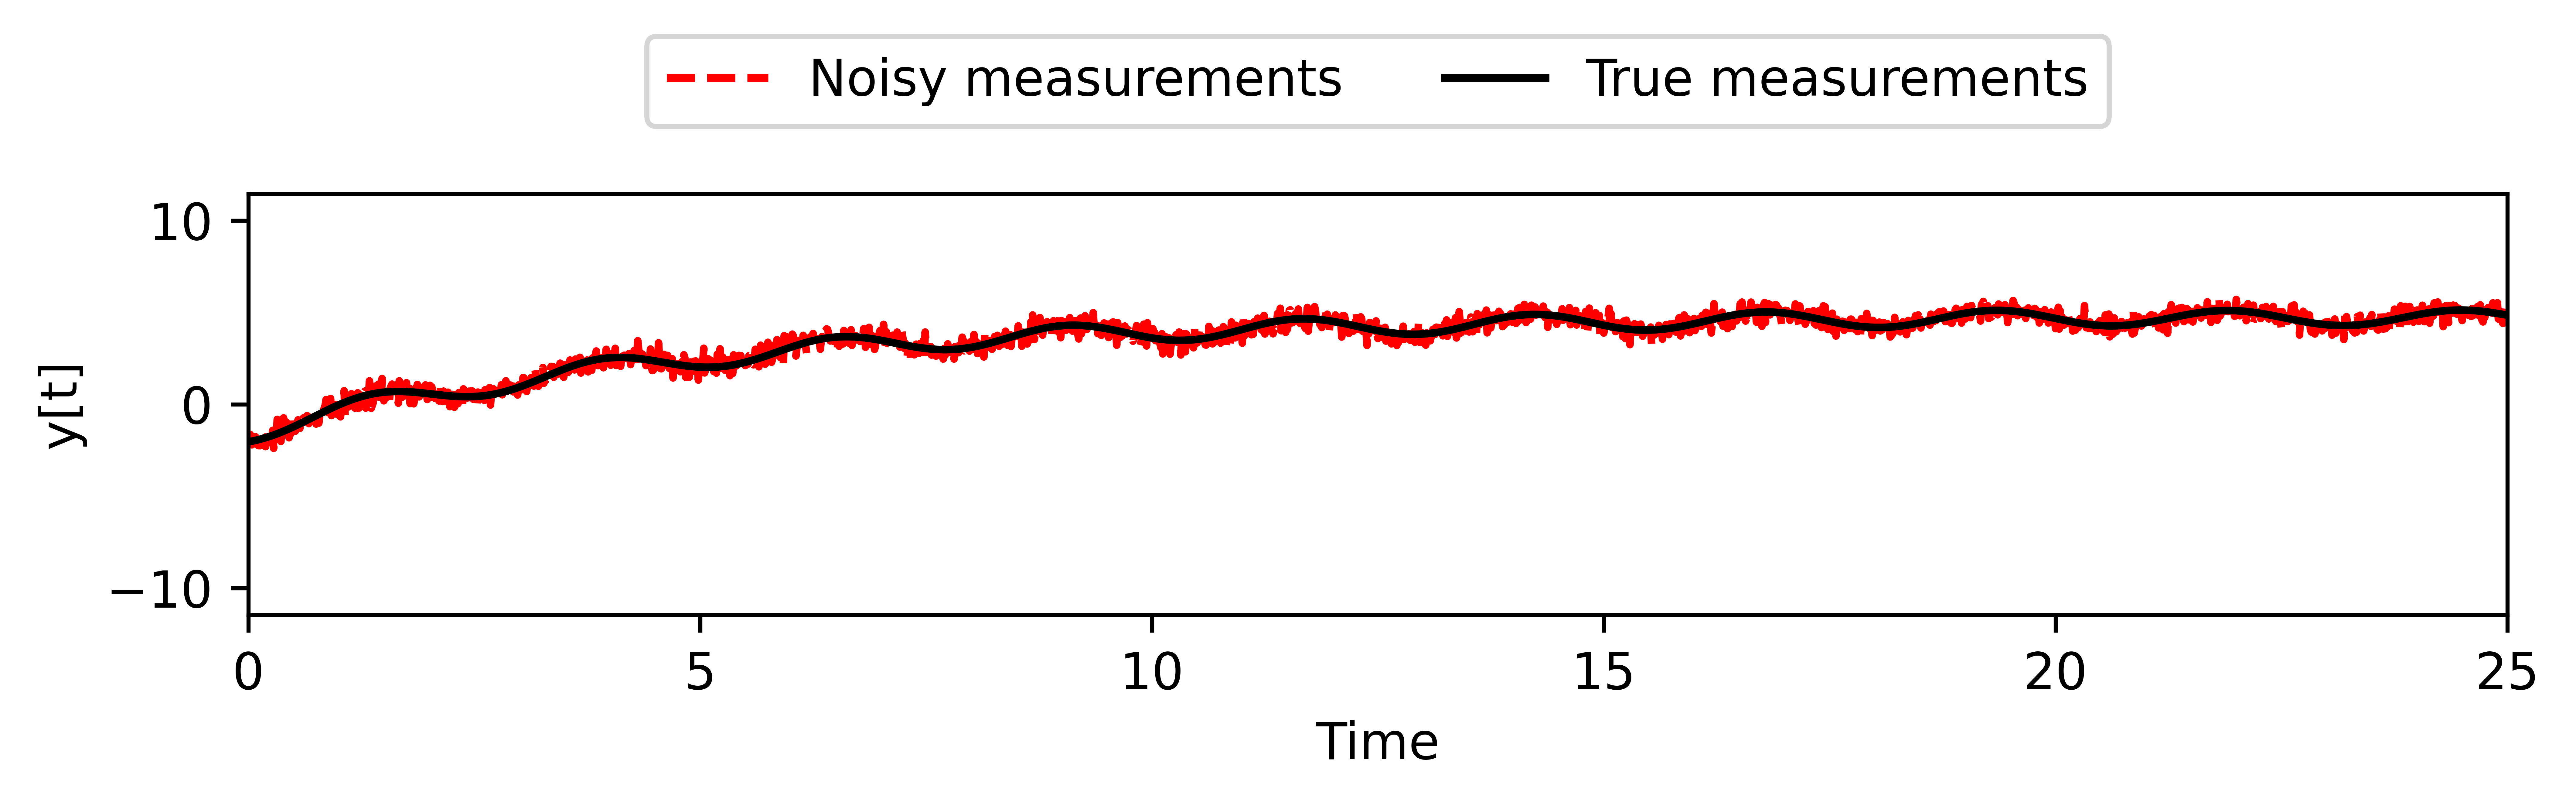
\includegraphics[width=\textwidth]{kalman_measurements.png}
  \end{minipage}
  \vfill
\end{frame}

\begin{frame}
  \vfill
  \[
    \minimize \quad \dfrac12 \sum_{t=0}^{T} \tikzmarknode{a}{\highlightdark{blue}{\norm{\vb{y}_t - \vb{Cx}_t}^2_{\inv{V}}}} + \dfrac12 \sum_{t=0}^{T-1} \tikzmarknode{b}{\highlightdark{red}{\norm{\vb{x}_{t+1} - \vb{Ax}_t}^2_{\inv{W}}}}
  \]
  \begin{tikzpicture}[overlay,remember picture,>=stealth,nodes={align=left,inner ysep=1pt},<-]
    \path (a.north) ++ (0,2em) node[anchor=south east,color=blue!67] (mass){Data fidelity};
    \draw [color=blue!87](a.north) |- ([xshift=-0.3ex,color=blue]mass.south west);

    \path (b.south) ++ (0,-2em) node[anchor=south east, color=red!67] (linop){Model fidelity};
    \draw [color=red!87](b.south) |- ([xshift=-0.3ex,color=red]linop.south west);
  \end{tikzpicture}
  \vfill
\end{frame}

\begin{frame}
  \vfill
  \small
  \[
    \begin{bmatrix}
      \Gram{C}+\Gram{A} & -\vb{A}^* \\
      -\vb{A}           & \Gram{C} + \vb{I} + \Gram{A}  & -\vb{A}^* \\
      & \ddots  & \ddots  & \ddots  \\
      &         & -\vb{A} & \Gram{C} + \vb{I} + \Gram{A}  & -\vb{A}^* \\
      &         &         & -\vb{A} & \Gram{C} + \vb{I}

    \end{bmatrix}
    \colvec{\hat{\vb{x}}_0, \hat{\vb{x}}_1, \vdots, \hat{\vb{x}}_{T-1}, \hat{\vb{x}}_T}
    =
    \colvec{\vb{C}^*\vb{y}_0, \vb{C}^*\vb{y}_1, \cdots, \vb{C}^*\vb{y}_{T-1}, \vb{C}^*\vb{y}_T}
  \]
  \vfill
\end{frame}

\begin{frame}
  \vfill
  \begin{minipage}{.38\textwidth}
    \centering
    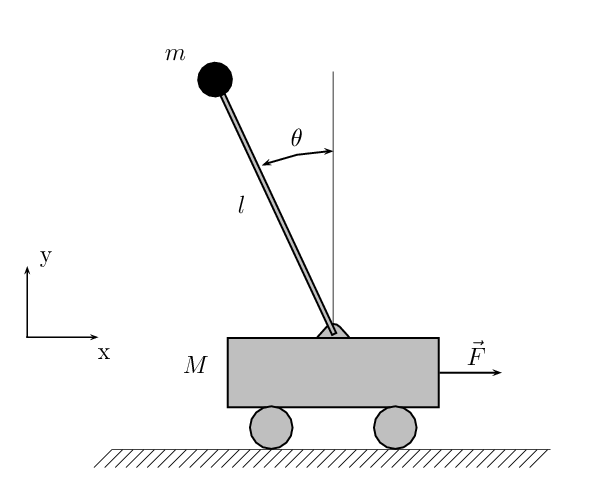
\includegraphics[width=\textwidth]{Cart-pendulum.png}
  \end{minipage}%
  \hfill
  \begin{minipage}{.58\textwidth}
    \centering
    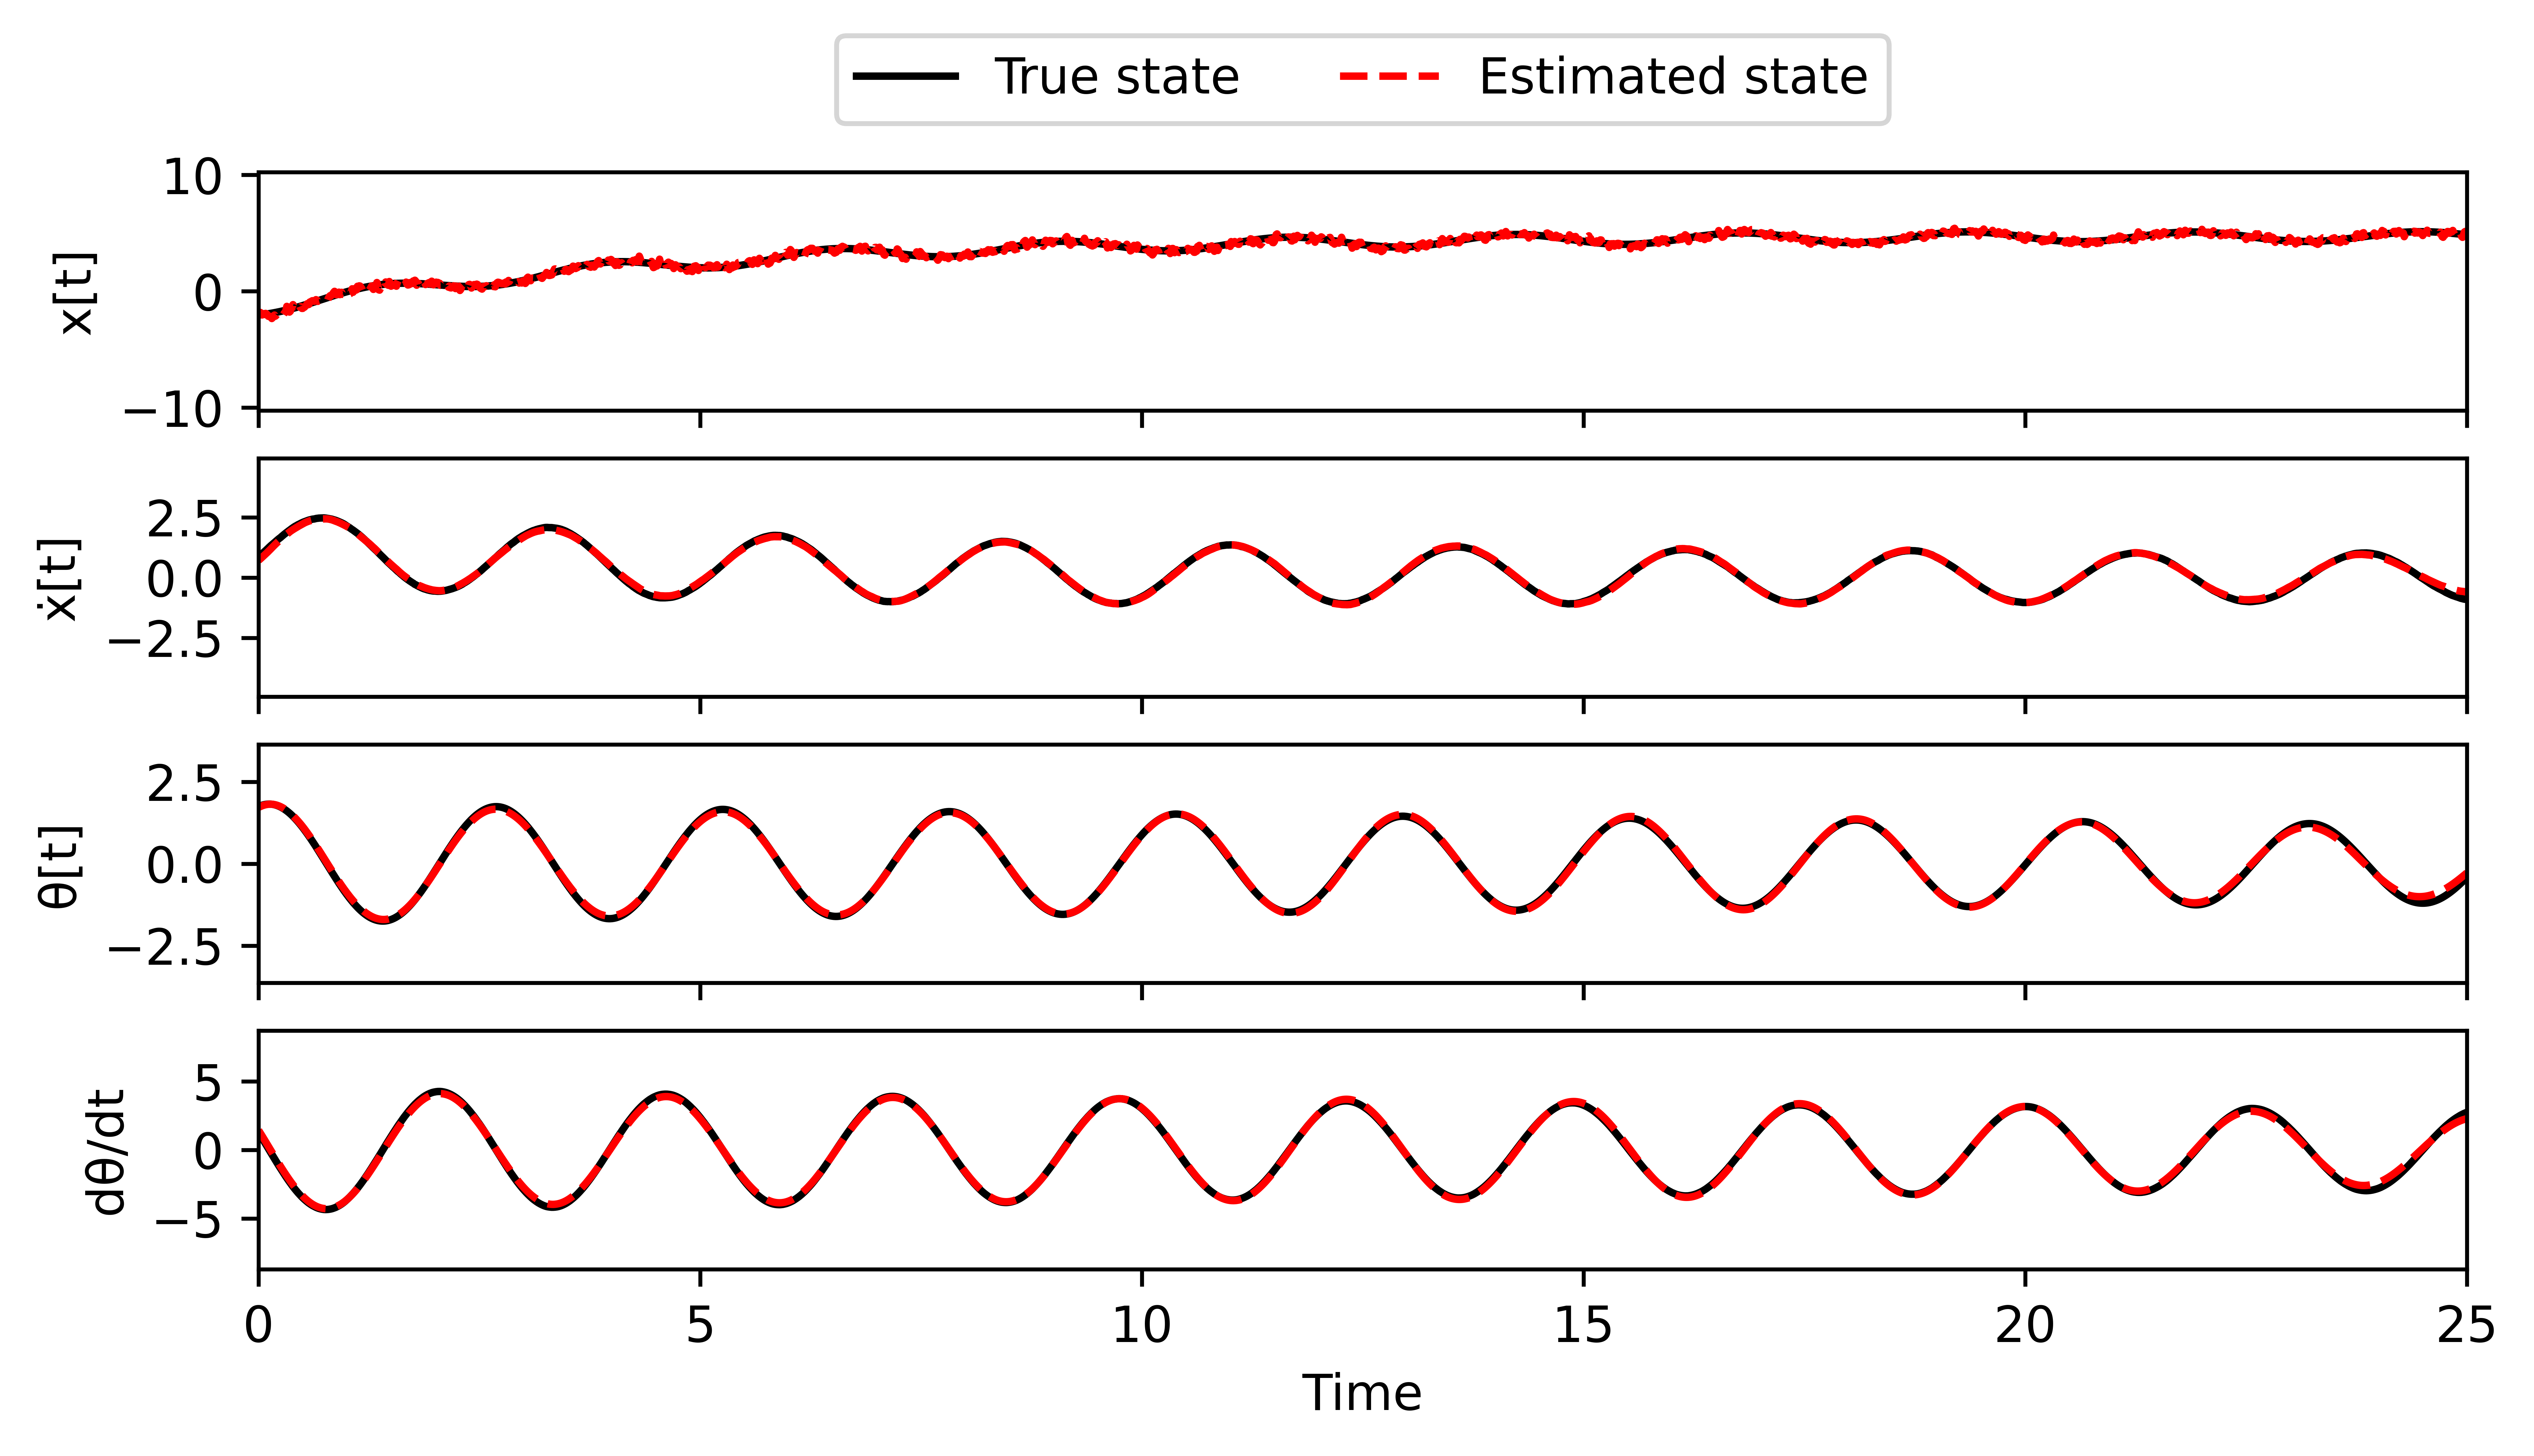
\includegraphics[width=\textwidth]{kalman_smoother.png}
  \end{minipage}
  \vfill
\end{frame}

\begin{frame}
  \vfill
  \begin{minipage}{.48\textwidth}
    \begin{itemize}
      \item Kalman smoothing fundamentally is a \emph{Multi-Objective} problem.
        \par
      \item The two objectives are competing against one another.
        \par
      \item Optimization problem is made tractable via \emph{scalarization}.
        \par
      \item Existence of a (convex) Pareto front.
    \end{itemize}
  \end{minipage}%
  \hfill
  \begin{minipage}{.48\textwidth}
    \centering
    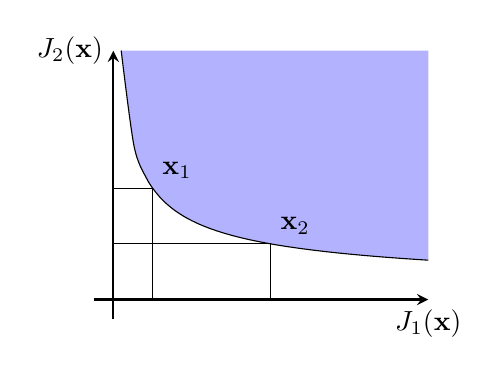
\begin{tikzpicture}[>=stealth]
      \fill[blue!30] (0.1, 3.16) -- plot[domain=0.1:4, smooth] (\x,{1/sqrt(\x)}) -- (4, 3.16) -- cycle;
      \draw[->, thick] (0,-.25) -- (0, 3.16) node [left] {$J_2(\vb{x})$};
      \draw[->, thick] (-.25,0) -- (4,0) node [below] {$J_1(\vb{x})$};
      \draw[domain=.1:4, smooth] plot (\x,{1/sqrt(\x)}); 

      \coordinate (A) at (2, 0.707);
      \node[above right] at (A) {$\vb{x}_2$};
      \draw (0, 0.707) -- (2, 0.707);
      \draw (2, 0) -- (2, 0.707);

      \coordinate (B) at (0.5, 1.414);
      \node[above right] at (B) {$\vb{x}_1$};
      \draw (0, 1.414) -- (0.5, 1.414);
      \draw (0.5, 0) -- (0.5, 1.414);
    \end{tikzpicture}
  \end{minipage}
  \vfill
\end{frame}

\section{Standard Scientific Computing}

\begin{frame}[standout, plain]
  \vfill
  {\usebeamerfont{title} Physics-Informed Neural Nets}

  {\usebeamerfont{subtitle} PDE and Scientific Computing}
  \vfill
\end{frame}

\begin{frame}
  \vfill
  \centering
  \[
    \left\{
      \begin{aligned}
        & \dfrac{\partial u}{\partial t} = \kappa \dfrac{\partial^2 u}{\partial x^2} \quad \text{for} \quad x \in \left]0, L\right[, \quad  t \in \left[0, T \right]  \\
        & u(0, t) = u(L, t) = 0 \\
        & u(x, 0) = \sin \left( \dfrac{\pi x}{L} \right).
      \end{aligned}
      \right.
    \]
    %
    \vfill
    \textbf{Analytical solution}  \hspace{1em}  \(  u(x, t) = \sin \left( \dfrac{\pi x}{L} \right) \exp \left( -\dfrac{\kappa \pi^2}{L^2} t \right) \)
    \vfill
\end{frame}

\begin{frame}
  \vfill
  \begin{minipage}{.38\textwidth}
    \centering
    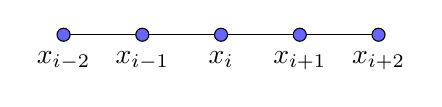
\begin{tikzpicture}
      \stencilpt{-2,0}{i-2}{$x_{i-2}$};
      \stencilpt{-1,0}{i-1}{$x_{i-1}$};
      \stencilpt{ 0,0}{i}  {$x_{i}$};
      \stencilpt{ 1,0}{i+1}{$x_{i+1}$};
      \stencilpt{ 2,0}{i+2}{$x_{i+2}$};
      \draw
      (i-2) -- (i-1)
      (i-1) -- (i)
      (i)   -- (i+1)
      (i+1) -- (i+2);
    \end{tikzpicture}
  \end{minipage}%
  \hfill
  \begin{minipage}{.58\textwidth}
    \begin{itemize}
      \item Space is typically discretized using a \emph{mesh}.
        \begin{itemize}
          \item Structured or unstructured mesh.
        \end{itemize}
        \par
      \item Differential operators are approximated on the discrete set of nodes.
        \begin{itemize}
          \item Finite differences, finite volumes, finite elements, \ldots
        \end{itemize}
        \par
      \item Temporal integration based on various numerical schemes.
        \begin{itemize}
          \item Euler, Runge-Kutta, Adam-Bashfort, \ldots
        \end{itemize}
    \end{itemize}
  \end{minipage}
  \vfill
\end{frame}

\begin{frame}
  \vfill
  \begin{minipage}{.38\textwidth}
    \centering
    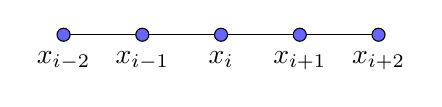
\begin{tikzpicture}
      \stencilpt{-2,0}{i-2}{$x_{i-2}$};
      \stencilpt{-1,0}{i-1}{$x_{i-1}$};
      \stencilpt{ 0,0}{i}  {$x_{i}$};
      \stencilpt{ 1,0}{i+1}{$x_{i+1}$};
      \stencilpt{ 2,0}{i+2}{$x_{i+2}$};
      \draw
      (i-2) -- (i-1)
      (i-1) -- (i)
      (i)   -- (i+1)
      (i+1) -- (i+2);
    \end{tikzpicture}
  \end{minipage}%
  \hfill
  \begin{minipage}{.58\textwidth}
    \centering
    \textbf{First-order derivative}
    %
    \[
      \dfrac{\partial u}{\partial x} = \dfrac{u_{i+1} - u_{i-1}}{2 \Delta x}  + \mathcal{O}(\Delta x^2)
    \]

    \bigskip

    \textbf{Second-order derivative}
    %
    \[
      \dfrac{\partial^2 u}{\partial x^2}  = \dfrac{u_{i+1} - 2u_i + u_{i-1}}{\Delta x^2} + \mathcal{O}(\Delta x^2)
    \]
  \end{minipage}
  \vfill
\end{frame}

\begin{frame}
  \vfill
  \centering
  \textbf{Semi-discretized system}

  \[
    \dfrac{\dd}{\dd t}  \colvec{u_1, u_2, u_3, u_4, u_5}
    =
    \dfrac{\kappa}{\Delta x^2}
    \begin{bmatrix}
      -2  & 1 \\
      1 & -2  & 1 \\
      & 1   & -2  & 1 \\
      &     & 1   & -2  & 1 \\
      &     &     & 1 & -2
    \end{bmatrix}
    \colvec{u_1, u_2, u_3, u_4, u_5}
  \]

  \vfill
\end{frame}

\begin{frame}
  \vfill
  \centering
  \begin{tabular}{l|c}
    \textbf{Explicit Euler} & \( \vb{u}_{t+1} = \left( \vb{I} + \Delta t \vb{L} \right) \vb{u}_t  \)  \\  \\
    \textbf{Implicit Euler} & \(  \vb{u}_{t+1}  = \left( \vb{I} - \Delta t \vb{L} \right)^{-1} \vb{u}_t \)  \\  \\
    \textbf{Crank-Nicholson}  & \(  \vb{u}_{t+1}  = \left(  \vb{I} - \dfrac{\Delta t}{2} \vb{L} \right)^{-1}  \left( \vb{I} + \dfrac{\Delta t}{2} \vb{L} \right) \vb{u}_t \)
  \end{tabular}
  \vfill
\end{frame}

\begin{frame}
  \vfill
  \begin{minipage}{.28\textwidth}
    \centering
    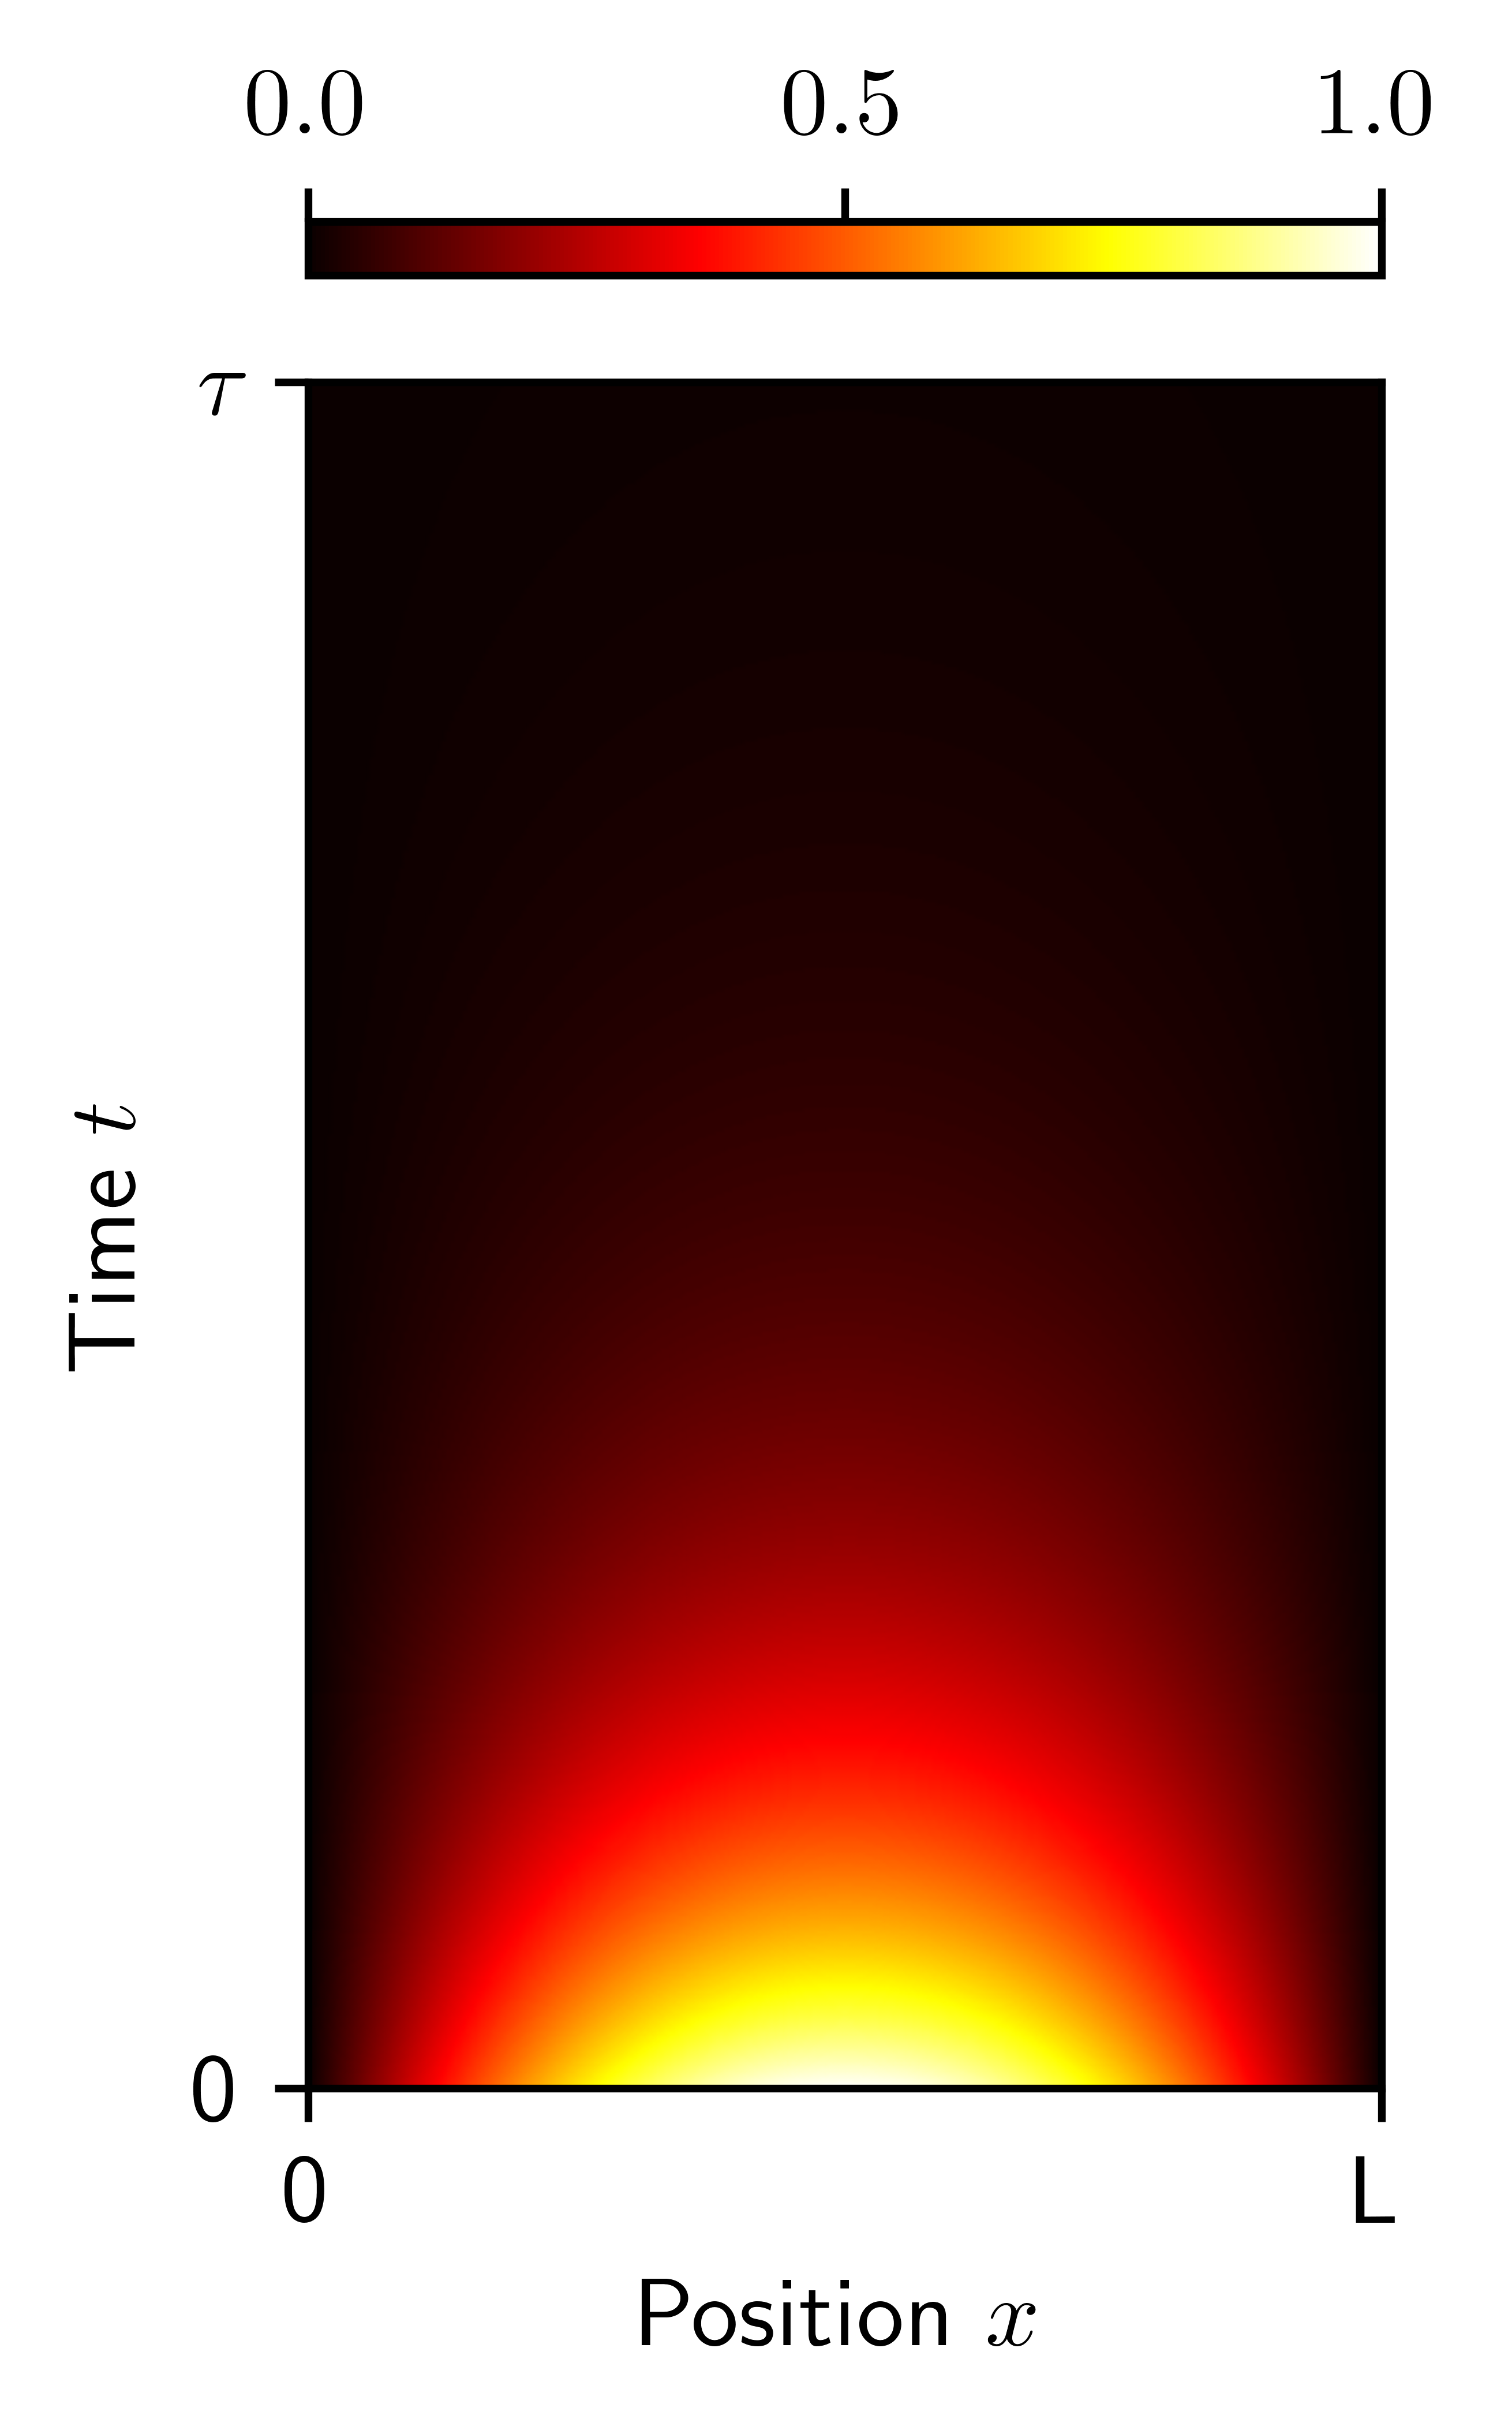
\includegraphics[width=\textwidth]{true_solution.png}
  \end{minipage}%
  \hfill
  \begin{minipage}{.68\textwidth}
    \begin{center}
      \color{Green}{\textbf{Pros} \hspace{1em}  \ding{52}}
    \end{center}
    %
    \par\bigskip
    \hrule
    %
    \par\bigskip
    \begin{itemize}
      \item Proof of consistency and convergence.
        \par
      \item Control of the approximation error, both in time $\mathcal{O}(\Delta t^n)$ and space $\mathcal{O}(\Delta x^m)$.
        \par
      \item Specialized solvers amenable to high-performance computing (HPC).
        \par
      \item Certification of existing CFD codes for sensitive applications.
    \end{itemize}
  \end{minipage}
\end{frame}

\begin{frame}
  \vfill
  \begin{minipage}{.28\textwidth}
    \centering
    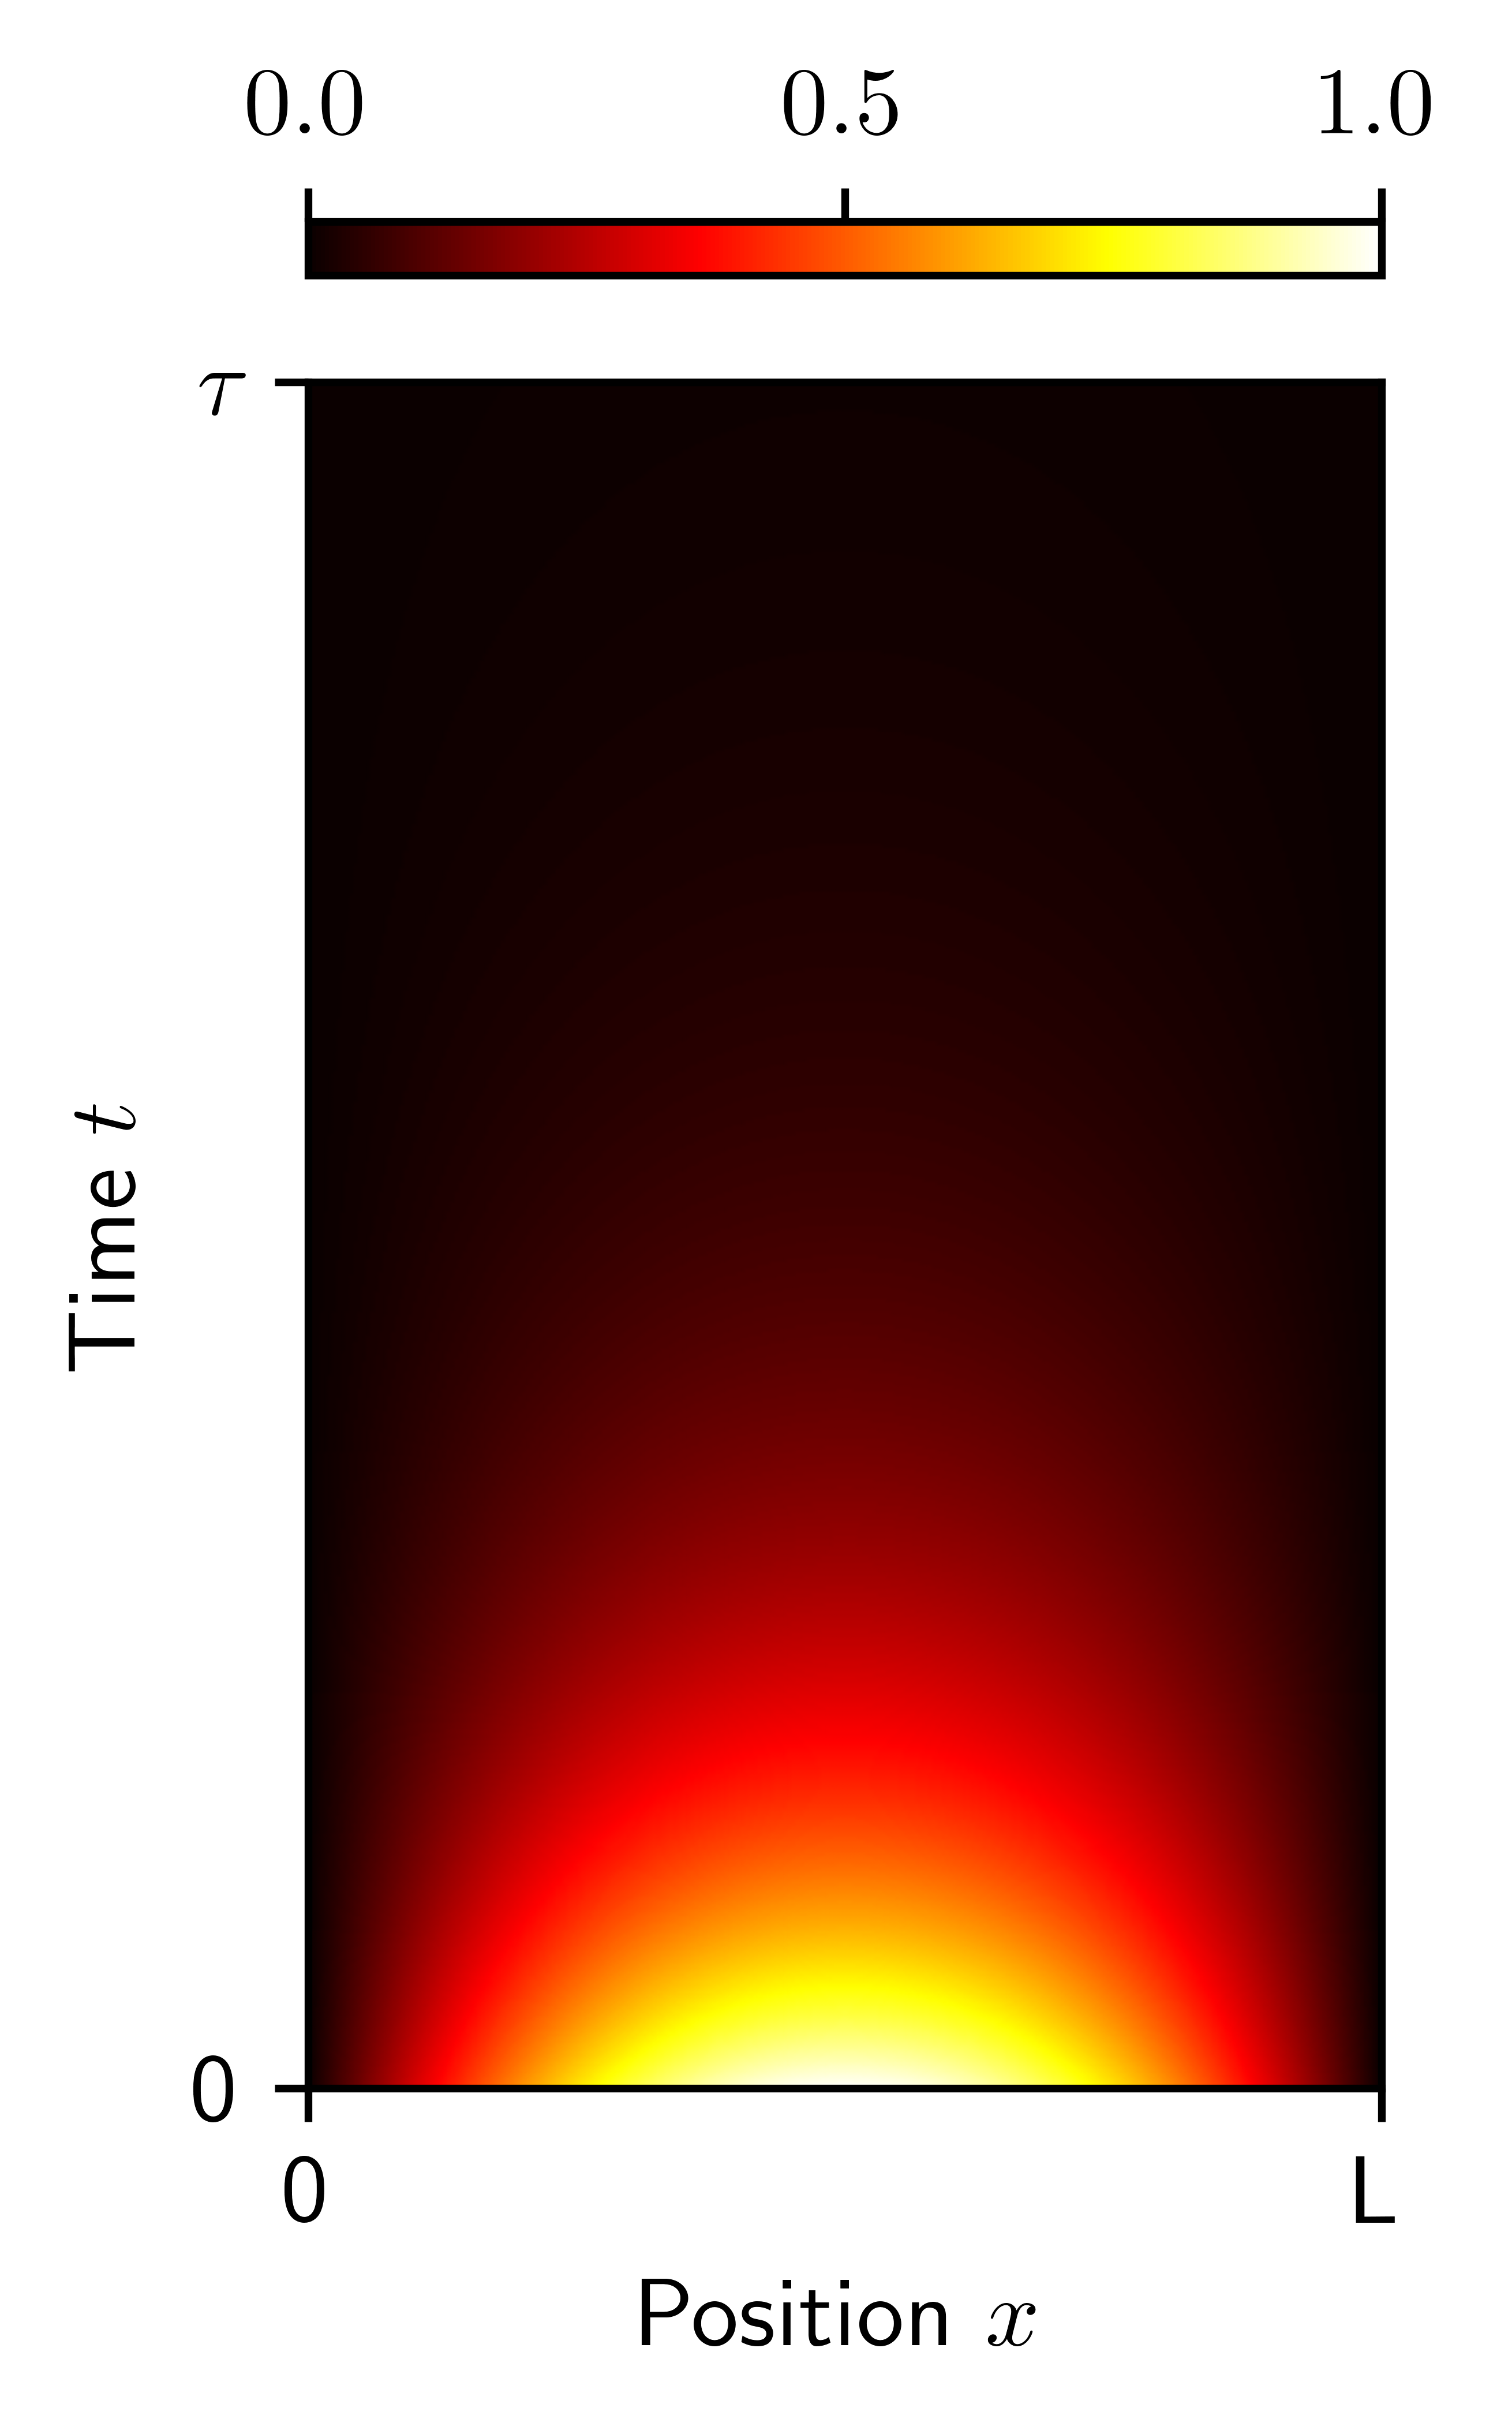
\includegraphics[width=\textwidth]{true_solution.png}
  \end{minipage}%
  \hfill
  \begin{minipage}{.68\textwidth}
    \begin{center}
      \color{Red}{\textbf{Cons} \hspace{1em}  \ding{55}}
    \end{center}
    %
    \par\bigskip
    \hrule
    %
    \par\bigskip
    \begin{itemize}
      \item Meshing complicated geometries is more of an art than science.
        \par
      \item Relatively high computational cost.
        \par
      \item Solver specialized for a single (type of) PDE.
        \par
      \item Constant need for code modernization to keep up-to-date with new processor architectures.
    \end{itemize}
  \end{minipage}
\end{frame}

\section{Physics-Informed Neural Nets}

\begin{frame}[standout, plain]
  \vfill
  {\usebeamerfont{title} Physics-Informed Neural Nets}

  {\usebeamerfont{subtitle} Back to deep learning}
  \vfill
\end{frame}

\begin{frame}
  \vfill
  \begin{minipage}{.68\textwidth}
    \begin{itemize}
      \item Proposed by Raissi, Perdikaris et Karniadakis in 2017 for solving PDE.
    \end{itemize}
    %
    \bigskip
    %
    \textbf{Idea}  \hspace{1em}  Leverage the universal approximation capabilities of neural nets to represent the solution to a PDE.
  \end{minipage}%
  \hfill
  \begin{minipage}{.28\textwidth}
    \centering
    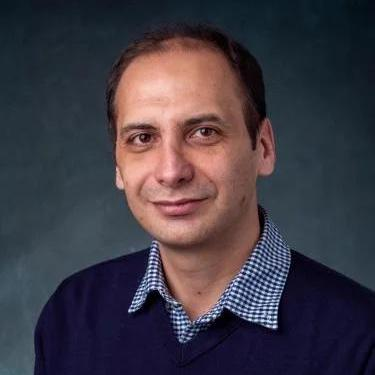
\includegraphics[width=\textwidth]{mazar_raissi.jpeg}
    \par
    {\tiny
    Maziar Raissi
    }
  \end{minipage}
  \vfill
\end{frame}

\begin{frame}
  \vfill
  \centering
  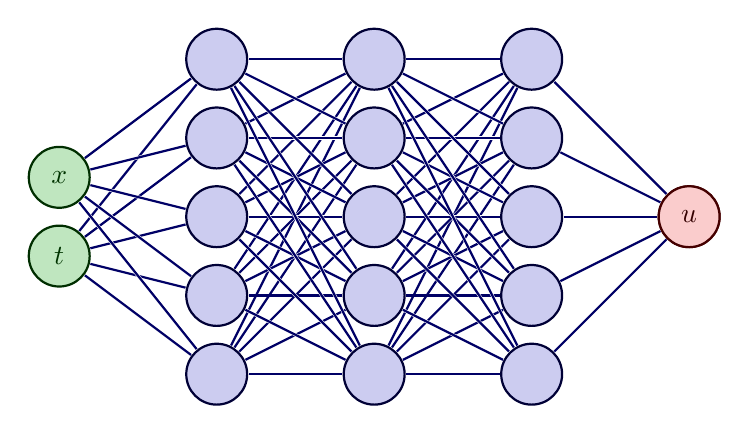
\begin{tikzpicture}[x=2cm,y=1cm]
    % \message{^^JNeural network without arrows}
    \readlist\Nnod{2,5,5,5,1} % array of number of nodes per layer

    % \message{^^J  Layer}
    \foreachitem \N \in \Nnod{ % loop over layers
      \def\lay{\Ncnt} % alias of index of current layer
      \pgfmathsetmacro\prev{int(\Ncnt-1)} % number of previous layer
      % \message{\lay,}
      \foreach \i [evaluate={\y=\N/2-\i; \x=\lay; \n=\nstyle;}] in {1,...,\N}{ % loop over nodes

        % NODES
        \ifnum \lay = 1
        \ifnum \i = 1
        \node[node \n] (N\lay-\i) at (\x,\y) {$x$};
        \else
        \node[node \n] (N\lay-\i) at (\x,\y) {$t$};
        \fi
        \else
        \node[node \n] (N\lay-\i) at (\x,\y) {};
        \fi

        \ifnum \lay = 5
        \node[node \n] (N\lay-\i) at (\x,\y) {$u$};
        \fi

        % CONNECTIONS
        \ifnum\lay>1 % connect to previous layer
        \foreach \j in {1,...,\Nnod[\prev]}{ % loop over nodes in previous layer
          \draw[connect,white,line width=1.2] (N\prev-\j) -- (N\lay-\i);
          \draw[connect] (N\prev-\j) -- (N\lay-\i);
          }
          \fi % else: nothing to connect first layer
          }
          }
  \end{tikzpicture} 
  \vfill
\end{frame}

\begin{frame}[fragile]{}
  \vfill
  \centering
  \begin{lstlisting}[language=Python]
  def u(x, t):
    return neural_net(tf.concat([t, x], 1), weights, biases)
  \end{lstlisting}
  \vfill
\end{frame}

\begin{frame}[fragile]{}
  \vfill
  \centering
  \begin{lstlisting}[language=Python]
  def residual(x, t, kappa):
    # Computation of the time-derivative.
    u_t = tf.gradients(u, t)[0]
    # Computation of the first spatial derivative.
    u_x = tf.gradients(u, x)[0]
    # Computation of the second spatial derivative.
    u_xx = tf.gradients(u_x, x)[0]
    # Definition of the residual.
    r = u_t - kappa*u_xx
    return r
  \end{lstlisting}
  \vfill
\end{frame}

\begin{frame}
  \vfill
  \[
    \begin{aligned}
      \mathrm{Find} & \quad \boldsymbol{\vartheta} \in \R^n \\
      \subto        & \quad \mathcal{R}(x, t) \equiv \dfrac{\partial u_{\vartheta}}{\partial t} - \kappa \dfrac{\partial^2 u_{\vartheta}}{\partial x^2} = 0 \quad \forall (x, t) \in \left[0, L\right] \times \left[0, T\right] \\
      & \quad u_{\vartheta}(x, 0) = u_0(x)  \\
      & \quad u_{\vartheta}(0, t) = u_{\vartheta}(L, t) = 0.
    \end{aligned}
  \]
  \vfill
\end{frame}

\begin{frame}
  \vfill
  \centering
  \begin{tabular}{l|c}
    \textbf{Physics}  & $\displaystyle \mathcal{L}_{\varphi}(\boldsymbol{\vartheta}) = \dfrac{1}{T \cdot L} \int_{0}^T \int_0^L  \abs{ \mathcal{R}(x, t) }^2 \ \dd x \dd t$  \\  \\
    \textbf{Initial condition}  & $\displaystyle \mathcal{L}_{IC}(\boldsymbol{\vartheta}) = \dfrac{1}{L} \int_0^L \abs{ u_{\vartheta}(x, 0) - u_0(x) }^2 \ \dd x $ \\  \\
    \textbf{Boundary conditions}  & $\displaystyle \mathcal{L}_{BC}(\boldsymbol{\vartheta}) = \dfrac{1}{T} \int_{0}^T \abs{ u_{\vartheta}(0, t) }^2 + \abs{ u_{\vartheta}(L, t) }^2 \ \dd t \)
  \end{tabular}
  \vfill
\end{frame}

\begin{frame}
  \vfill
  \centering
  \[
    \minimize_{\boldsymbol{\vartheta} \in \R^n} \quad \tikzmarknode{a}{\highlightdark{blue}{\alpha_1 \mathcal{L}_{IC}(\boldsymbol{\vartheta}) + \alpha_2 \mathcal{L}_{BC}(\boldsymbol{\vartheta})}} + \tikzmarknode{b}{\highlightdark{red}{\alpha_3 \mathcal{L}_{\varphi}(\boldsymbol{\vartheta})}}
  \]
  \begin{tikzpicture}[overlay,remember picture,>=stealth,nodes={align=left,inner ysep=1pt},<-]
    \path (a.north) ++ (0,2em) node[anchor=south east,color=blue!67] (mass){Data fidelity};
    \draw [color=blue!87](a.north) |- ([xshift=-0.3ex,color=blue]mass.south west);

    \path (b.south) ++ (0,-2em) node[anchor=south east, color=red!67] (linop){Model fidelity};
    \draw [color=red!87](b.south) |- ([xshift=-0.3ex,color=red]linop.south west);
  \end{tikzpicture}

  \vspace{1em}

  with $\alpha_1 + \alpha_2 + \alpha_3 = 1$.
  \vfill
\end{frame}

\begin{frame}
  \vfill
  \begin{minipage}{.28\textwidth}
    \centering
    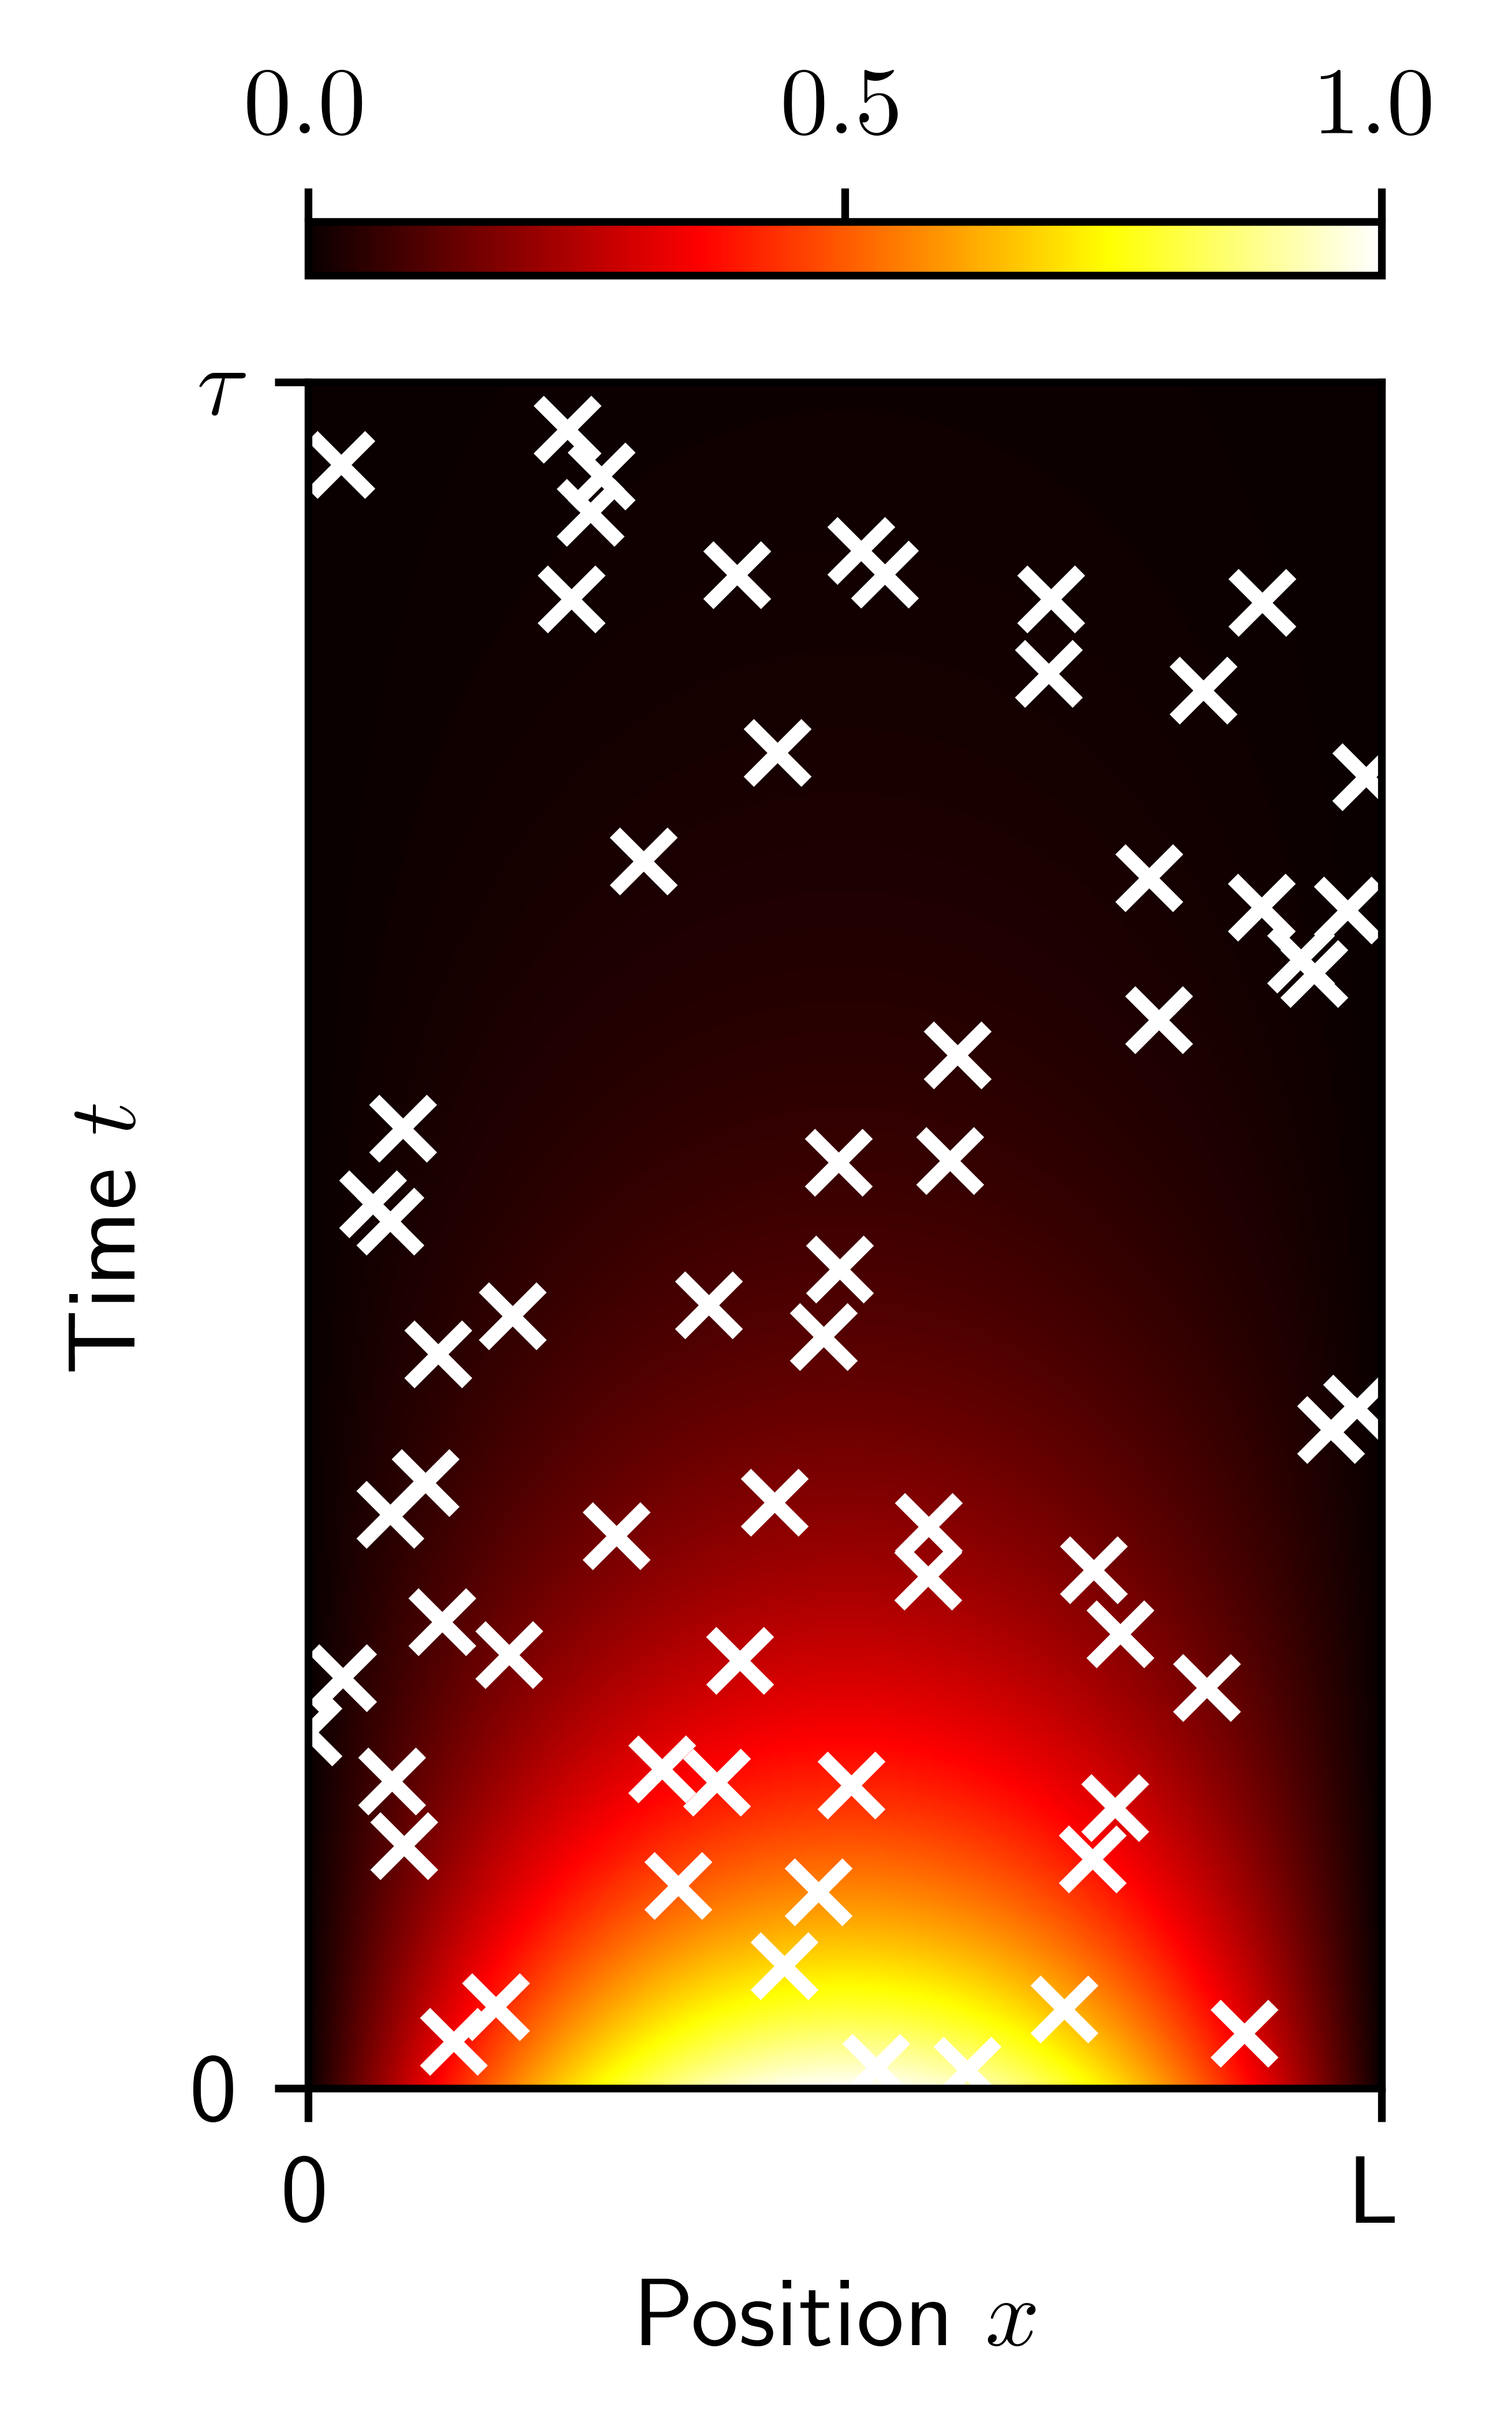
\includegraphics[width=\textwidth]{spatio_temporal_sampling.png}
  \end{minipage}%
  \hfill
  \begin{minipage}{.68\textwidth}
    \[
      \begin{aligned}
        \mathcal{L}_{\varphi}(\boldsymbol{\vartheta}) & = \dfrac{1}{T \cdot L} \int_{0}^{T} \int_{0}^{L} \abs{\mathcal{R}(x, t)}^2 \ \dd x \dd t  \\
          & \simeq \dfrac{1}{N_{\varphi}} \sum_{i=1}^{N_{\varphi}} \abs{ \mathcal{R}(x_i, t_i) }^2
      \end{aligned}
    \]
  \end{minipage}
  \vfill
\end{frame}

\begin{frame}
  \vfill
  \begin{minipage}{.28\textwidth}
    \centering
    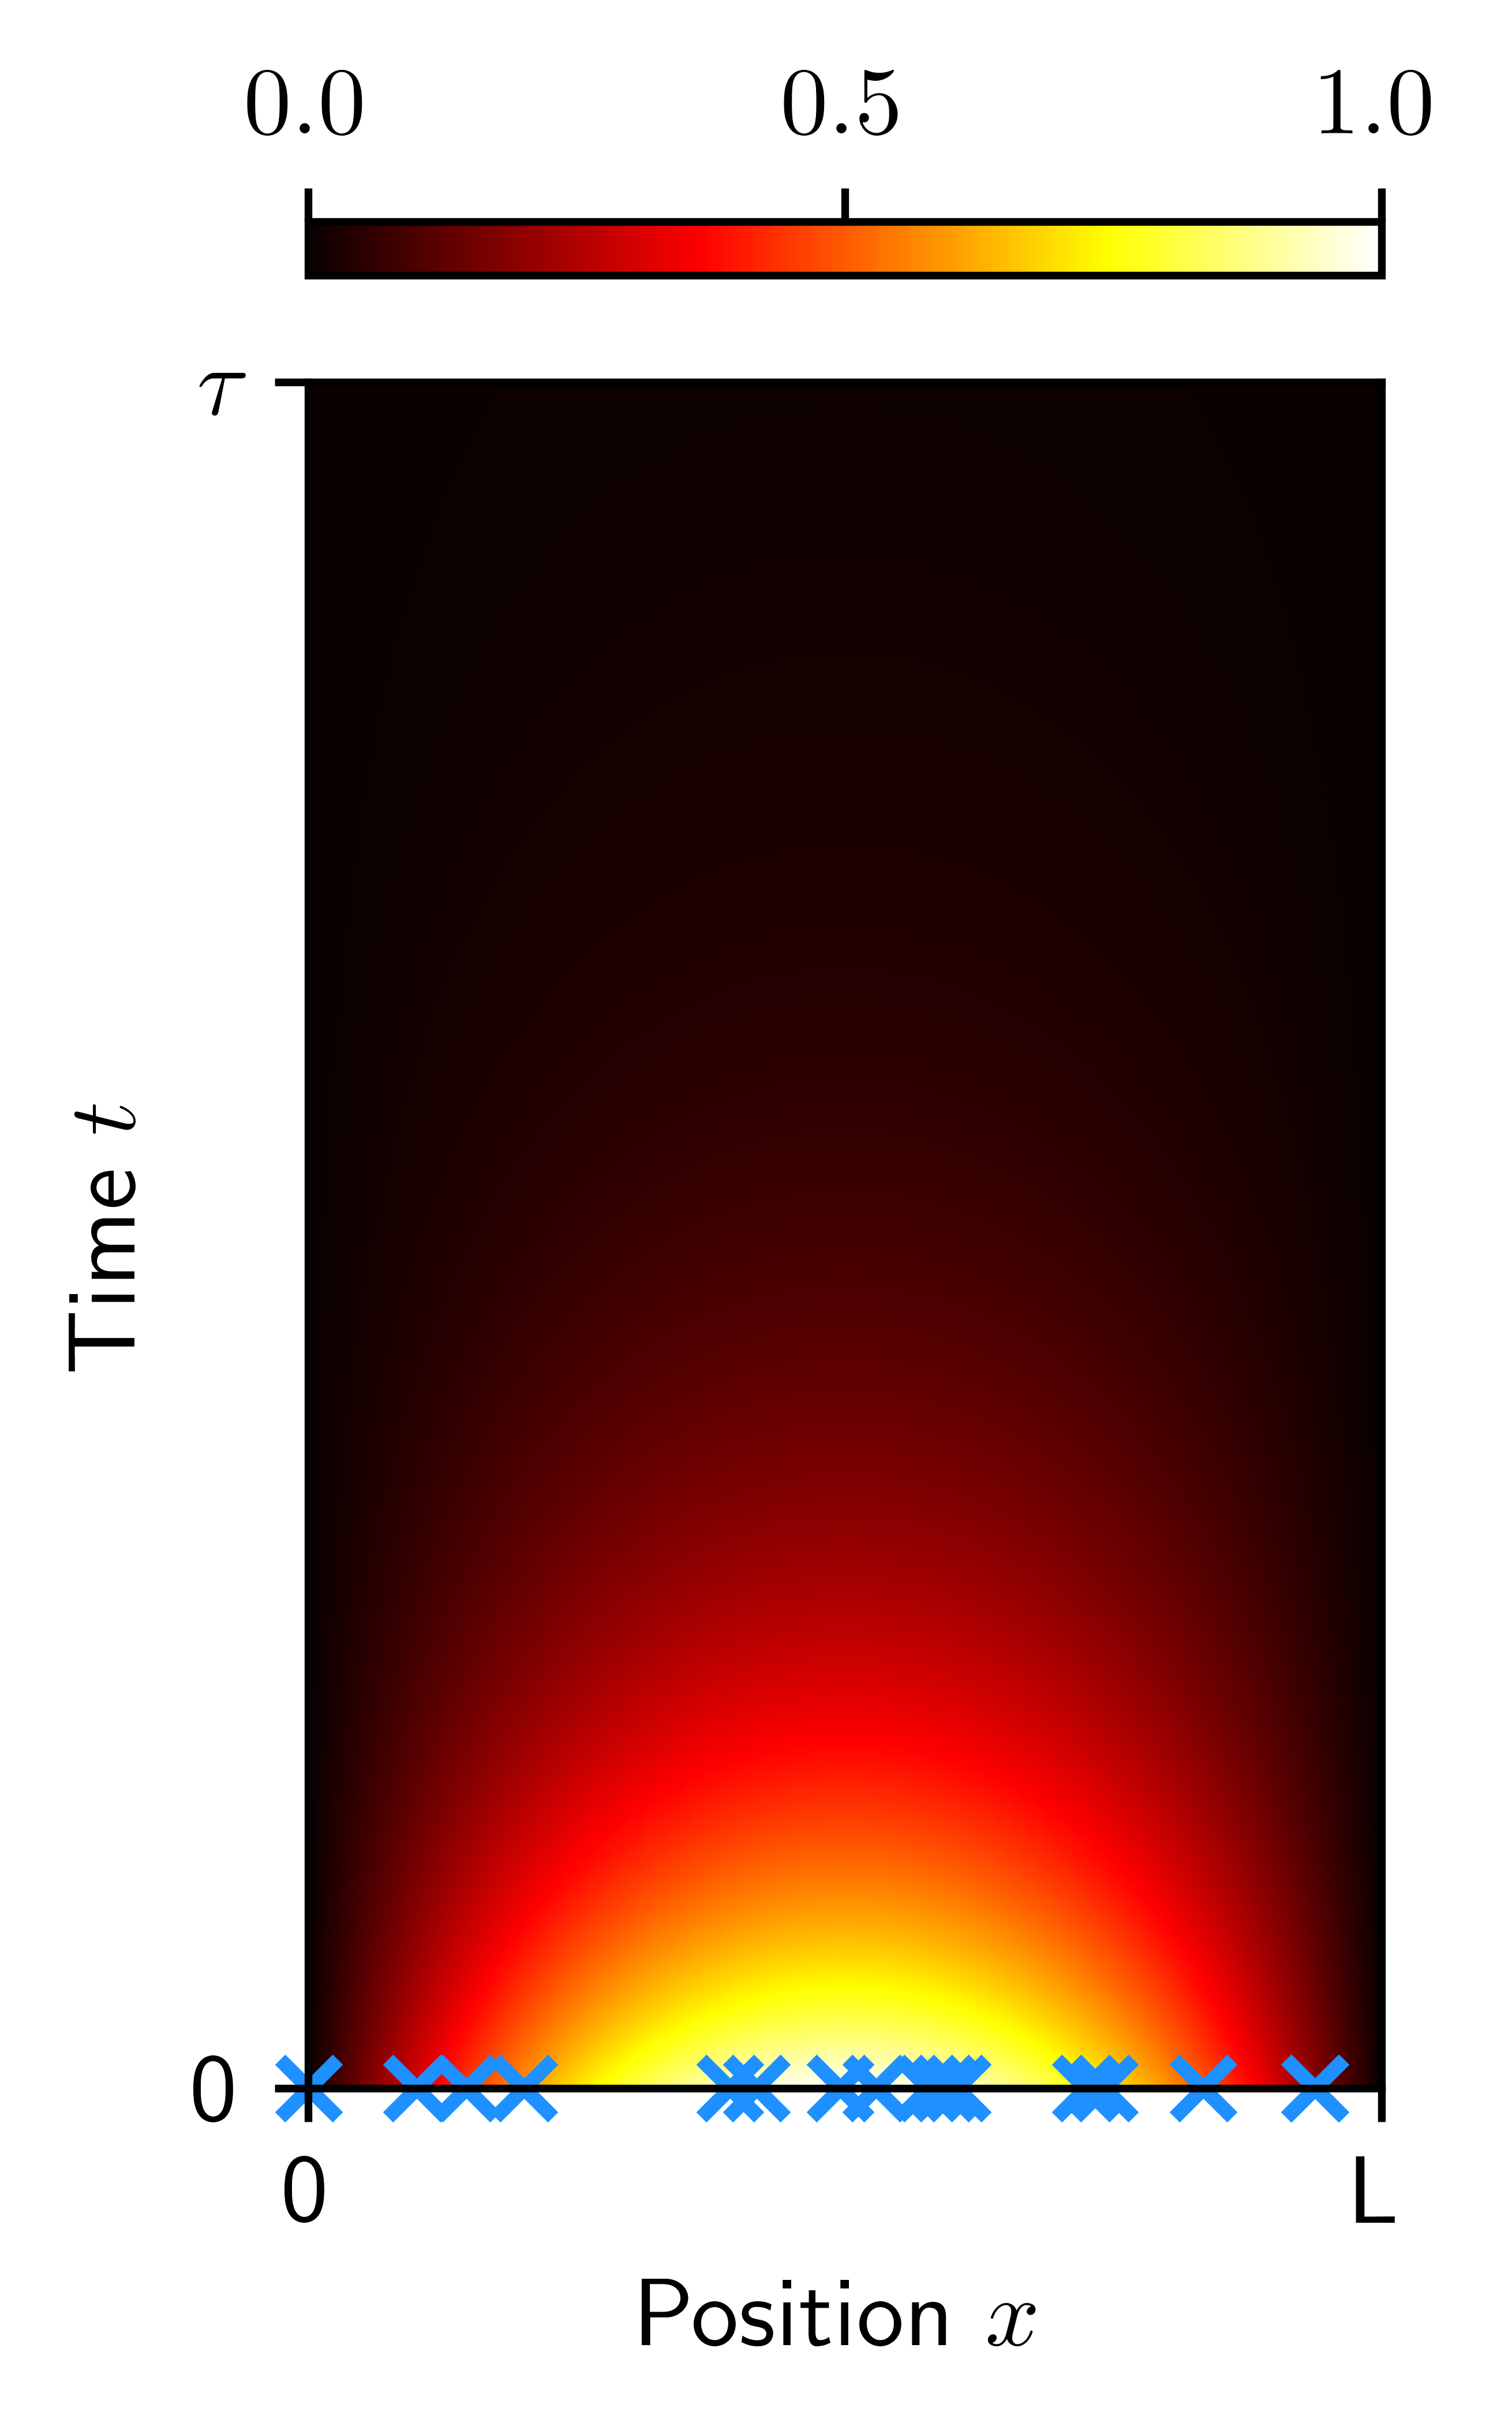
\includegraphics[width=\textwidth]{initial_condition_sampling.png}
  \end{minipage}%
  \hfill
  \begin{minipage}{.68\textwidth}
    \[
      \begin{aligned}
        \mathcal{L}_{IC}(\boldsymbol{\vartheta}) &  = \dfrac{1}{L} \int_{0}^{L} \abs{ u_{\vartheta}(x, 0) - u_0(x) }^2 \ \dd x  \\
          & \simeq \dfrac{1}{N_{IC}} \sum_{i=1}^{N_{IC}} \abs{ u_{\vartheta}(x_i, 0) - u_0(x_i) }^2
      \end{aligned}
    \]
  \end{minipage}
  \vfill
\end{frame}

\begin{frame}
  \vfill
  \begin{minipage}{.28\textwidth}
    \centering
    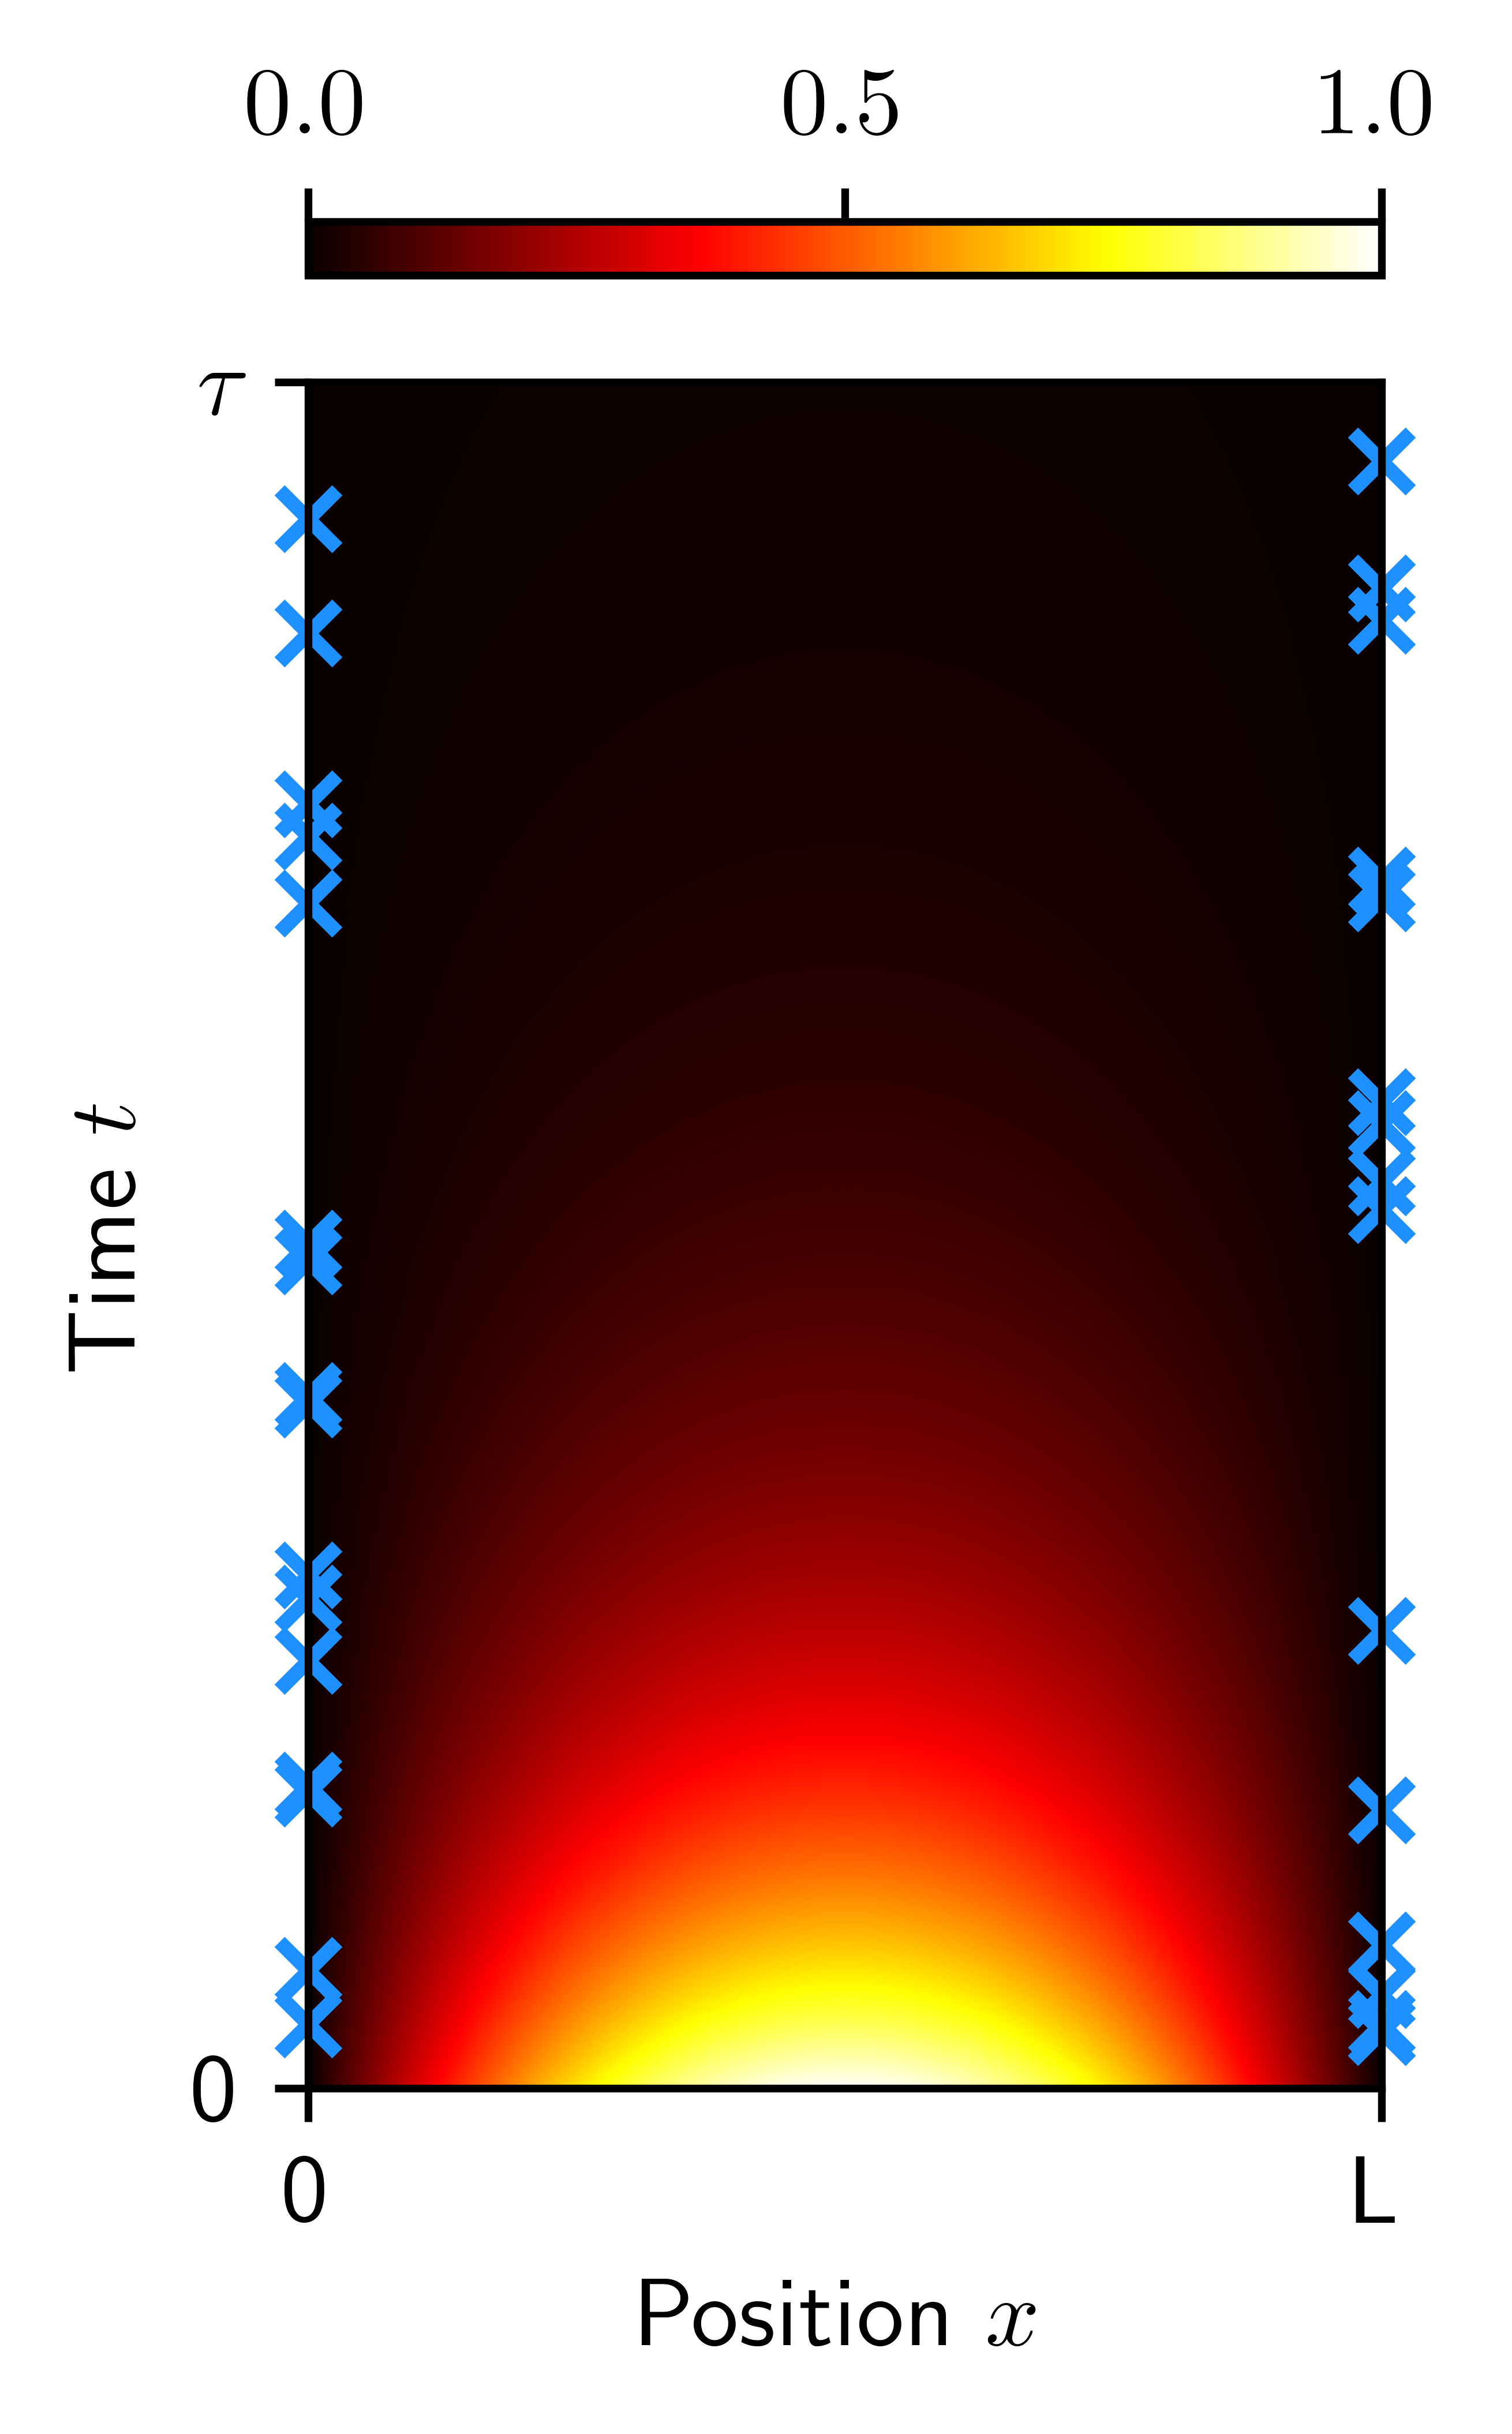
\includegraphics[width=\textwidth]{boundary_conditions_sampling.png}
  \end{minipage}%
  \hfill
  \begin{minipage}{.68\textwidth}
    \[
      \begin{aligned}
        \mathcal{L}_{BC}(\boldsymbol{\vartheta}) &  = \dfrac{1}{T} \int_{0}^{T} \abs{ u_\vartheta(0, t) }^2 + \abs{u_{\vartheta}(L, t)}^2 \ \dd t \\
          & = \dfrac{1}{N_{BC}} \sum_{i=1}^{N_{BC}} \abs{ u_{\vartheta}(0, t_i) }^2 + \abs{ u_{\vartheta}(L, t_i) }^2
      \end{aligned}
    \]
  \end{minipage}
  \vfill
\end{frame}

\begin{frame}
  \vfill
  \centering
  \textbf{Non-dimensionalization of the PDE}
  \vfill
  \begin{minipage}{.28\textwidth}
    \begin{overprint}
      \onslide<1-2>
      \[
        \hat{t} = \dfrac{t}{\tau}, \quad \hat{x} = \dfrac{x}{L}
      \]
      \onslide<3>
      \[
        \tau = \dfrac{L^2}{\kappa}
      \]
    \end{overprint}
  \end{minipage}%
  \hfill
  \begin{minipage}{.68\textwidth}
    \centering
    \begin{overprint}
      \onslide<1>
      \[
        \dfrac{\partial u}{\partial t} - \kappa \dfrac{\partial^2 u}{\partial x^2}  = 0
      \]

      \onslide<2>
      \[
        \dfrac{1}{\tau}  \dfrac{\partial u}{\partial \hat{t}}  - \dfrac{\kappa}{L^2} \dfrac{\partial^2 u}{\partial \hat{x}^2}  = 0
      \]

      \onslide<3>
      \[
        \dfrac{\kappa}{L^2} \left( \dfrac{\partial u}{\partial \hat{t}} - \dfrac{\partial^2 u}{\partial \hat{x}^2} \right) = 0
      \]
    \end{overprint}
  \end{minipage}
  \vfill
\end{frame}

\begin{frame}
  \vfill
  \begin{minipage}{.28\textwidth}
    \[
      \begin{aligned}
        \mathcal{R}(x, t) & \sim \dfrac{\kappa}{L^2}  \\  \\
        \text{data} & \sim 1
      \end{aligned}
    \]
  \end{minipage}%
  \hfill
  \begin{minipage}{.68\textwidth}
    Physics loss and data losses have fundamentally different scales, depending implicitly on  the system's parameters via the diffusive time-scale $\tau = \nicefrac{L^2}{\kappa}$.
    %
    \par\bigskip
    %
    \begin{itemize}
      \item If $\tau \gg 1$ --  Diffusion is very slow and the scale of data residuals is pre-dominant.
        %
      \item If $\tau \ll 1$ -- Diffusion is very fast and the scale of the physics residuals is pre-dominant.
    \end{itemize}
    \par\bigskip
    $\Longrightarrow$ Geometry of the Pareto front not only depends on $\alpha_1$, $\alpha_2$ and $\alpha_3$ but also on $\tau$ !
  \end{minipage}
  \vfill
\end{frame}

\begin{frame}
  \vfill
  \begin{minipage}{.38\textwidth}
    \centering
    \begin{tabular}{l|c}
      \textbf{Architecture} & MLP \\
      \textbf{Hidden layers} & 2  \\
      \textbf{Neurons per layer}  & 5  \\
      \textbf{Activation} & $\mathrm{sigmoid}$ \\  \\
      \hline  \\
      \textbf{Optimizer}  & ADAM  \\
      \textbf{Learning rate}  & $0.01$  \\
      \textbf{Epochs} & $10^5$
    \end{tabular}
  \end{minipage}%
  \hfill
  \begin{minipage}{.58\textwidth}
    \centering
    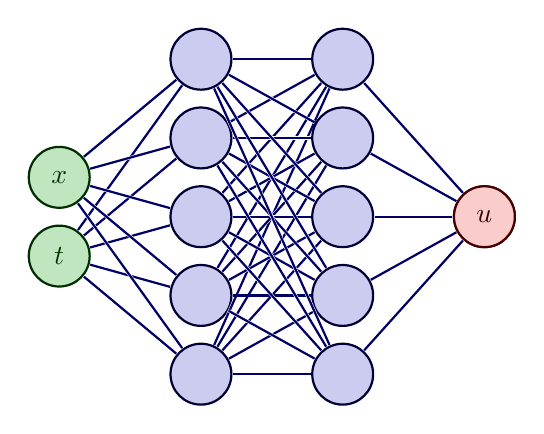
\begin{tikzpicture}[x=1.8cm,y=1cm]
      % \message{^^JNeural network without arrows}
      \readlist\Nnod{2,5,5,1} % array of number of nodes per layer

      % \message{^^J  Layer}
      \foreachitem \N \in \Nnod{ % loop over layers
        \def\lay{\Ncnt} % alias of index of current layer
        \pgfmathsetmacro\prev{int(\Ncnt-1)} % number of previous layer
        % \message{\lay,}
        \foreach \i [evaluate={\y=\N/2-\i; \x=\lay; \n=\nstyle;}] in {1,...,\N}{ % loop over nodes

          % NODES
          \ifnum \lay = 1
          \ifnum \i = 1
          \node[node \n] (N\lay-\i) at (\x,\y) {$x$};
          \else
          \node[node \n] (N\lay-\i) at (\x,\y) {$t$};
          \fi
          \else
          \node[node \n] (N\lay-\i) at (\x,\y) {};
          \fi

          \ifnum \lay = 4
          \node[node \n] (N\lay-\i) at (\x,\y) {$u$};
          \fi

          % CONNECTIONS
          \ifnum\lay>1 % connect to previous layer
          \foreach \j in {1,...,\Nnod[\prev]}{ % loop over nodes in previous layer
            \draw[connect,white,line width=1.2] (N\prev-\j) -- (N\lay-\i);
            \draw[connect] (N\prev-\j) -- (N\lay-\i);
            }
            \fi % else: nothing to connect first layer
            }
            }
    \end{tikzpicture} 
  \end{minipage}
  \vfill
\end{frame}

\begin{frame}
  \vfill
  \centering
  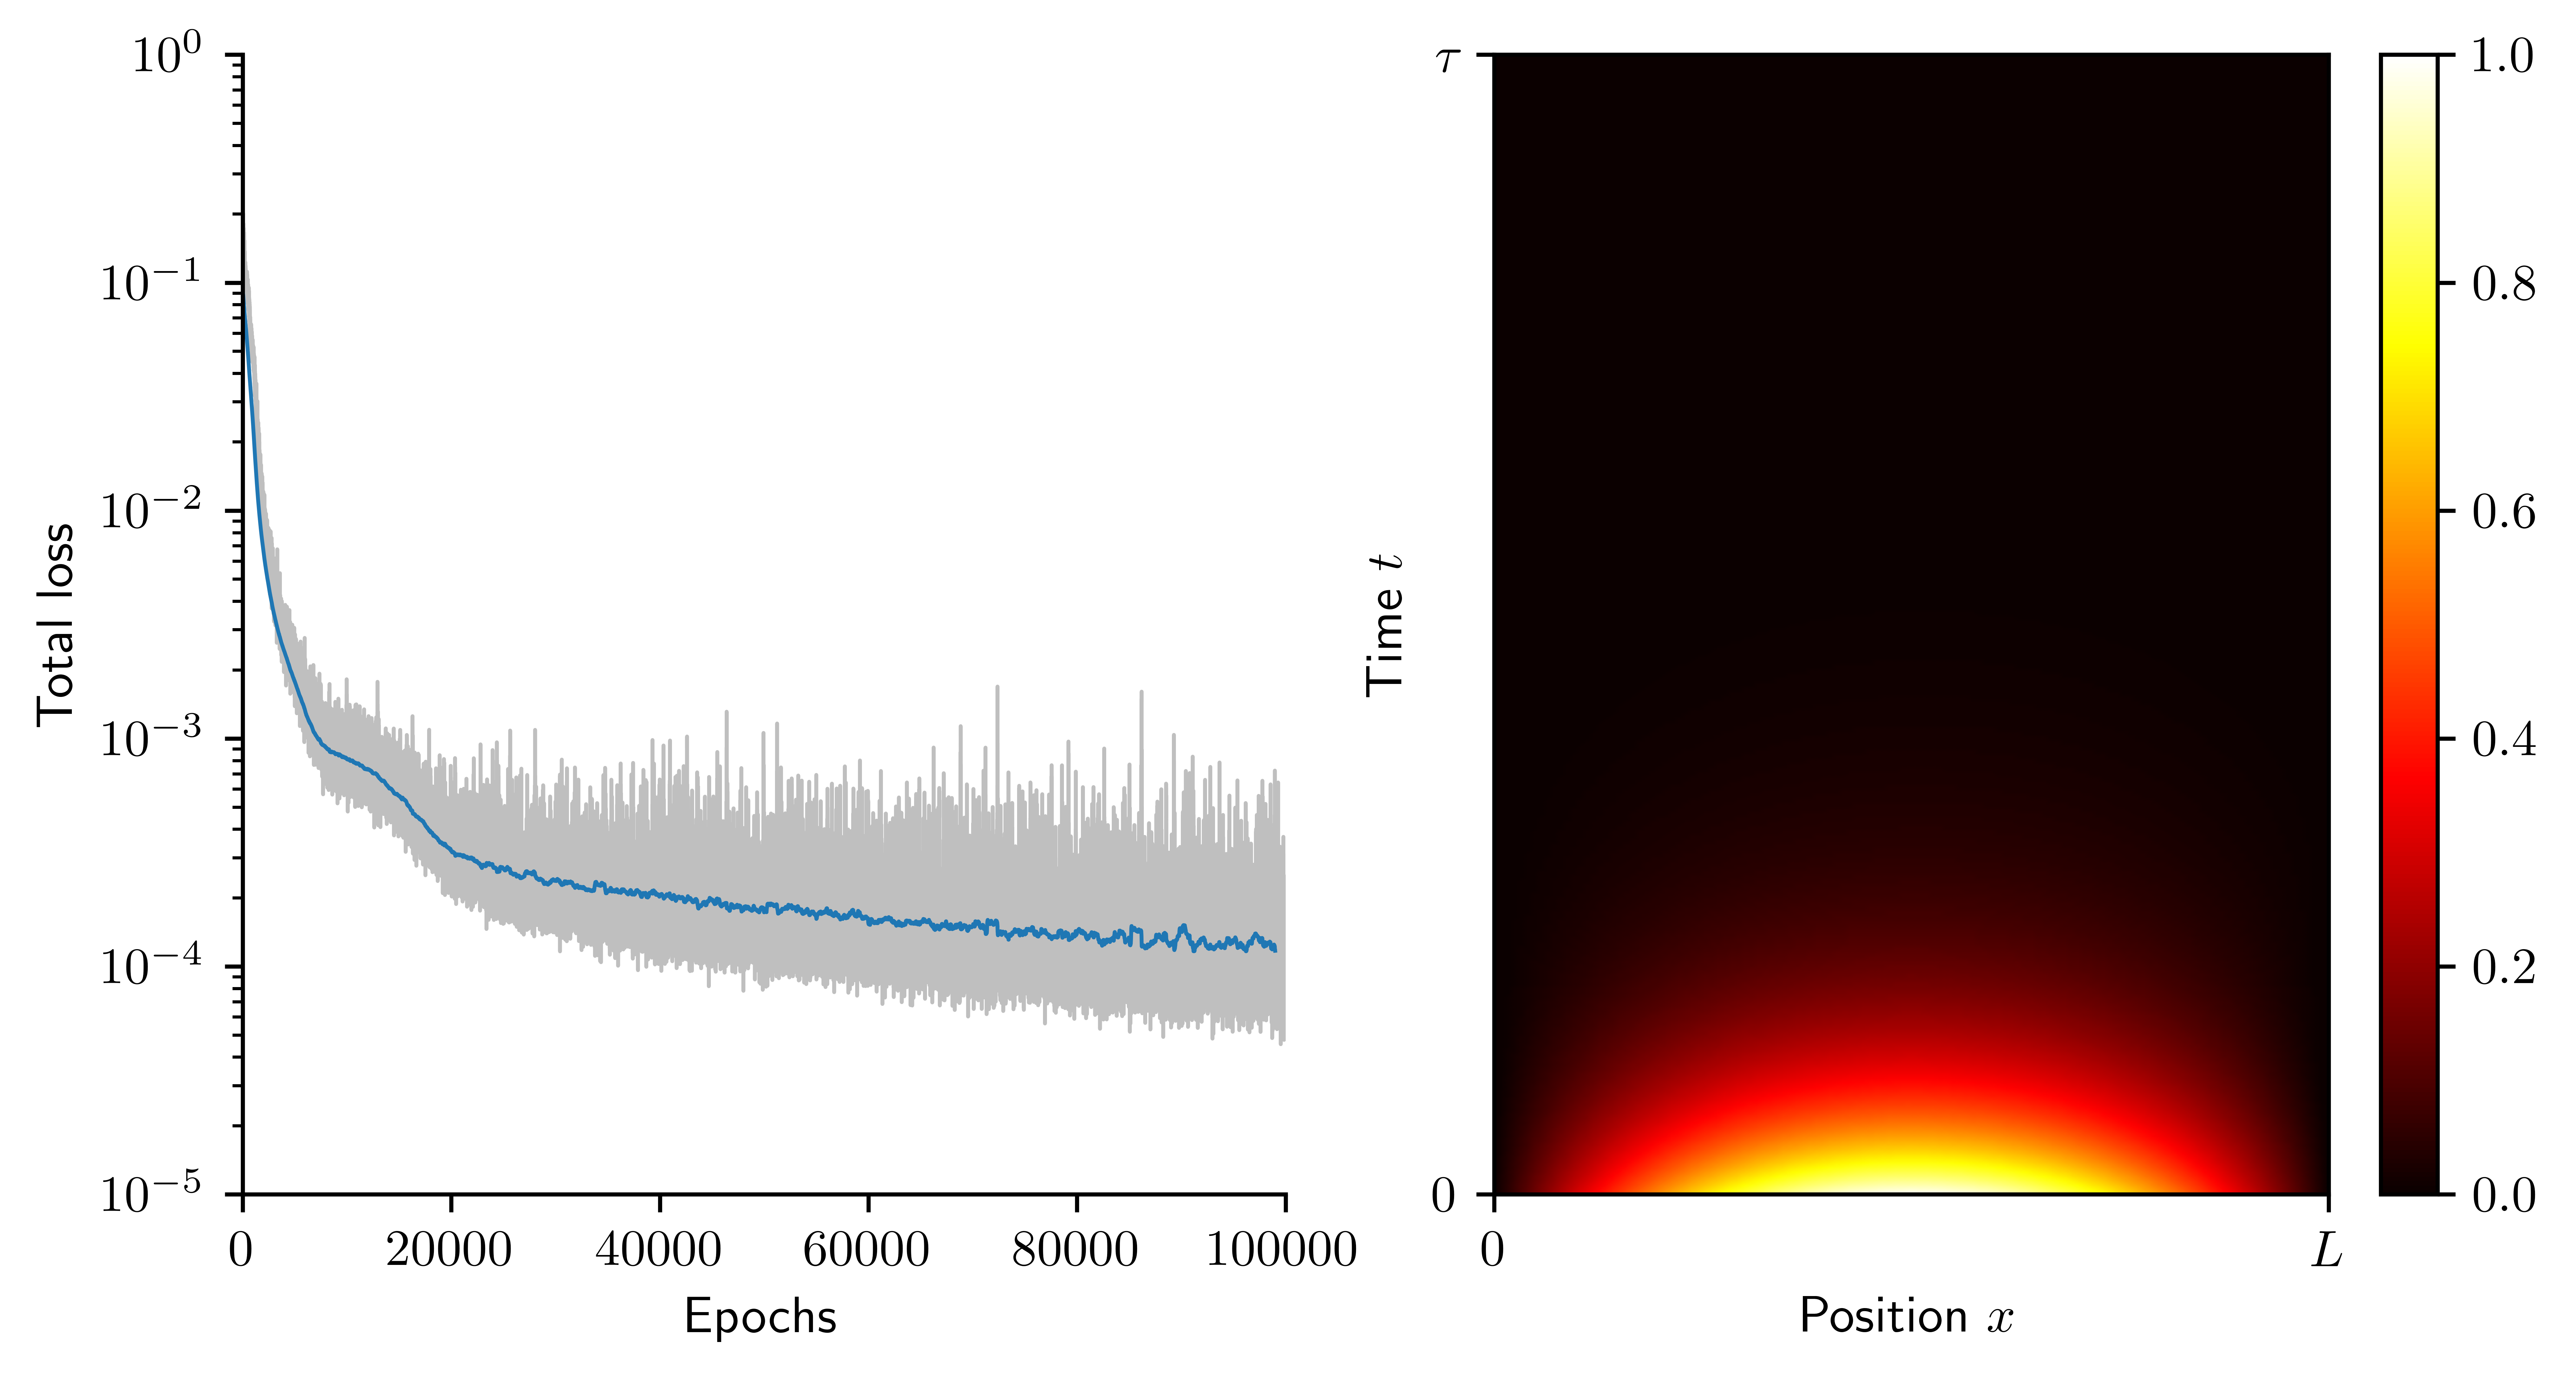
\includegraphics[width=.8\textwidth]{pinn_training.png}
  \par
  \small
  \textbf{Figure} : Convergence history (left) and spatio-temporal diagram of the approximate solution (right) for the parameters $(\kappa, L) = (1, 1)$.
  \vfill
\end{frame}

\begin{frame}
  \vfill
  \centering
  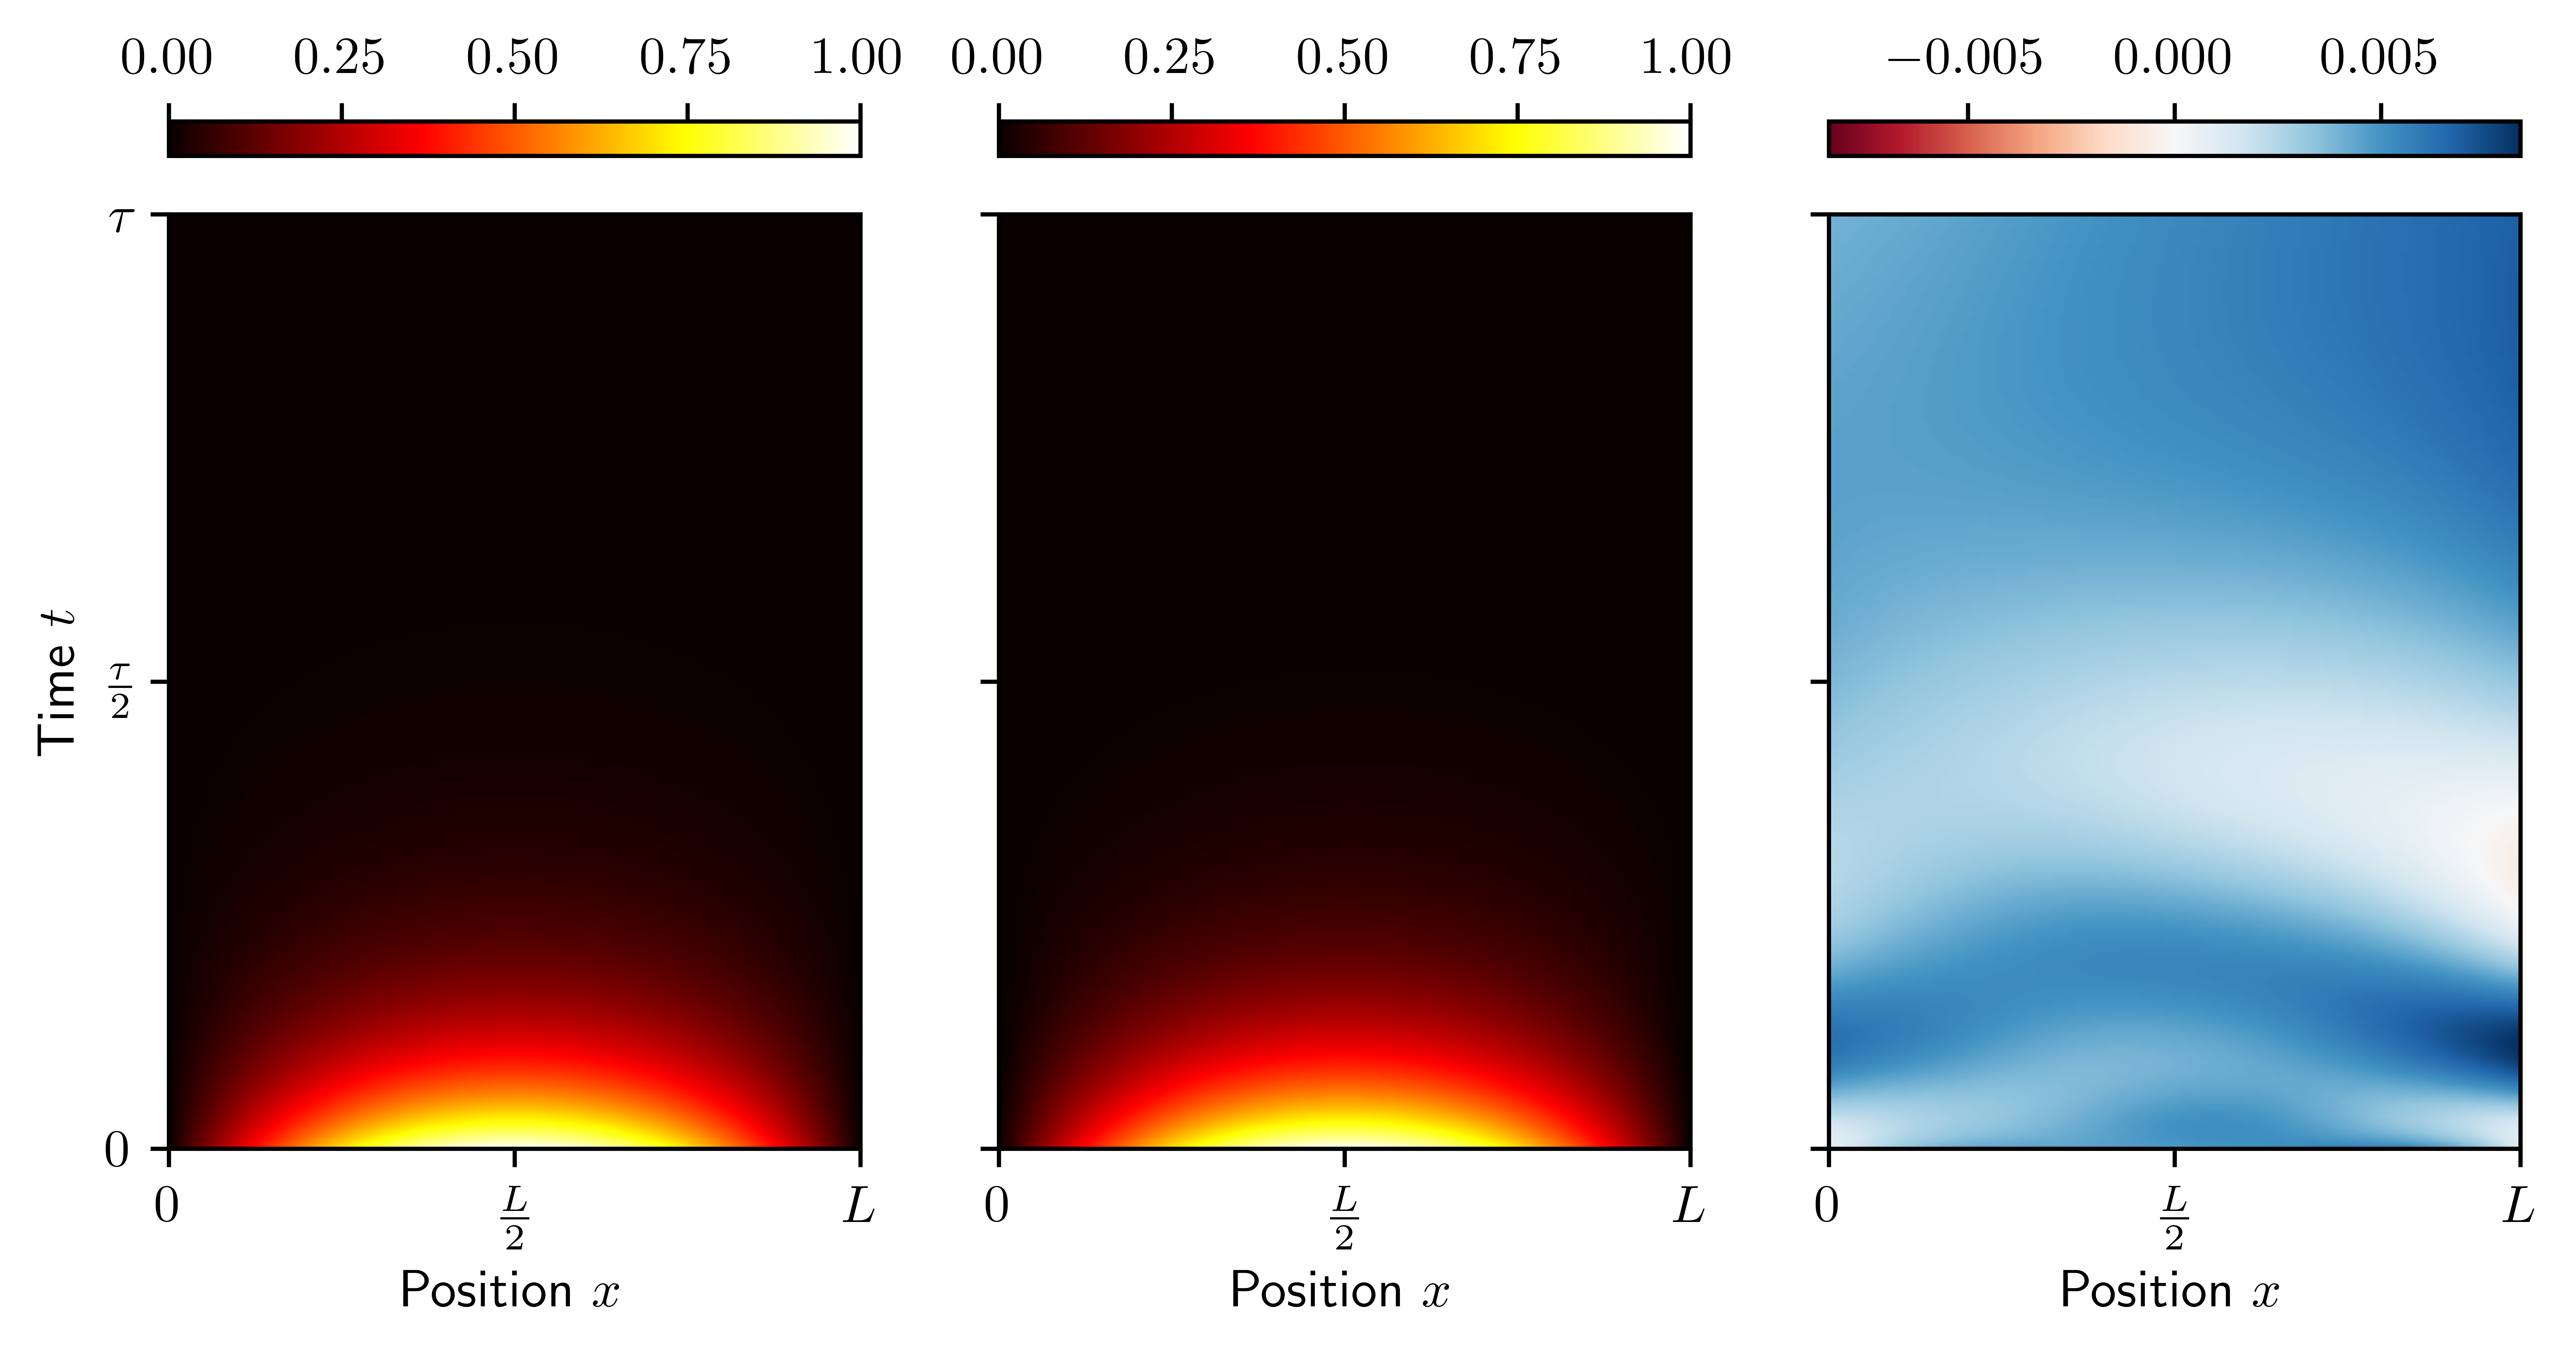
\includegraphics[width=.8\textwidth]{error.png}
  \par
  \small
  \textbf{Figure :} Ground truth solution (left), approximate solution (center), pointwise error (right).
  \vfill
\end{frame}

\begin{frame}
  \vfill
  \begin{minipage}{.38\textwidth}
    \centering
    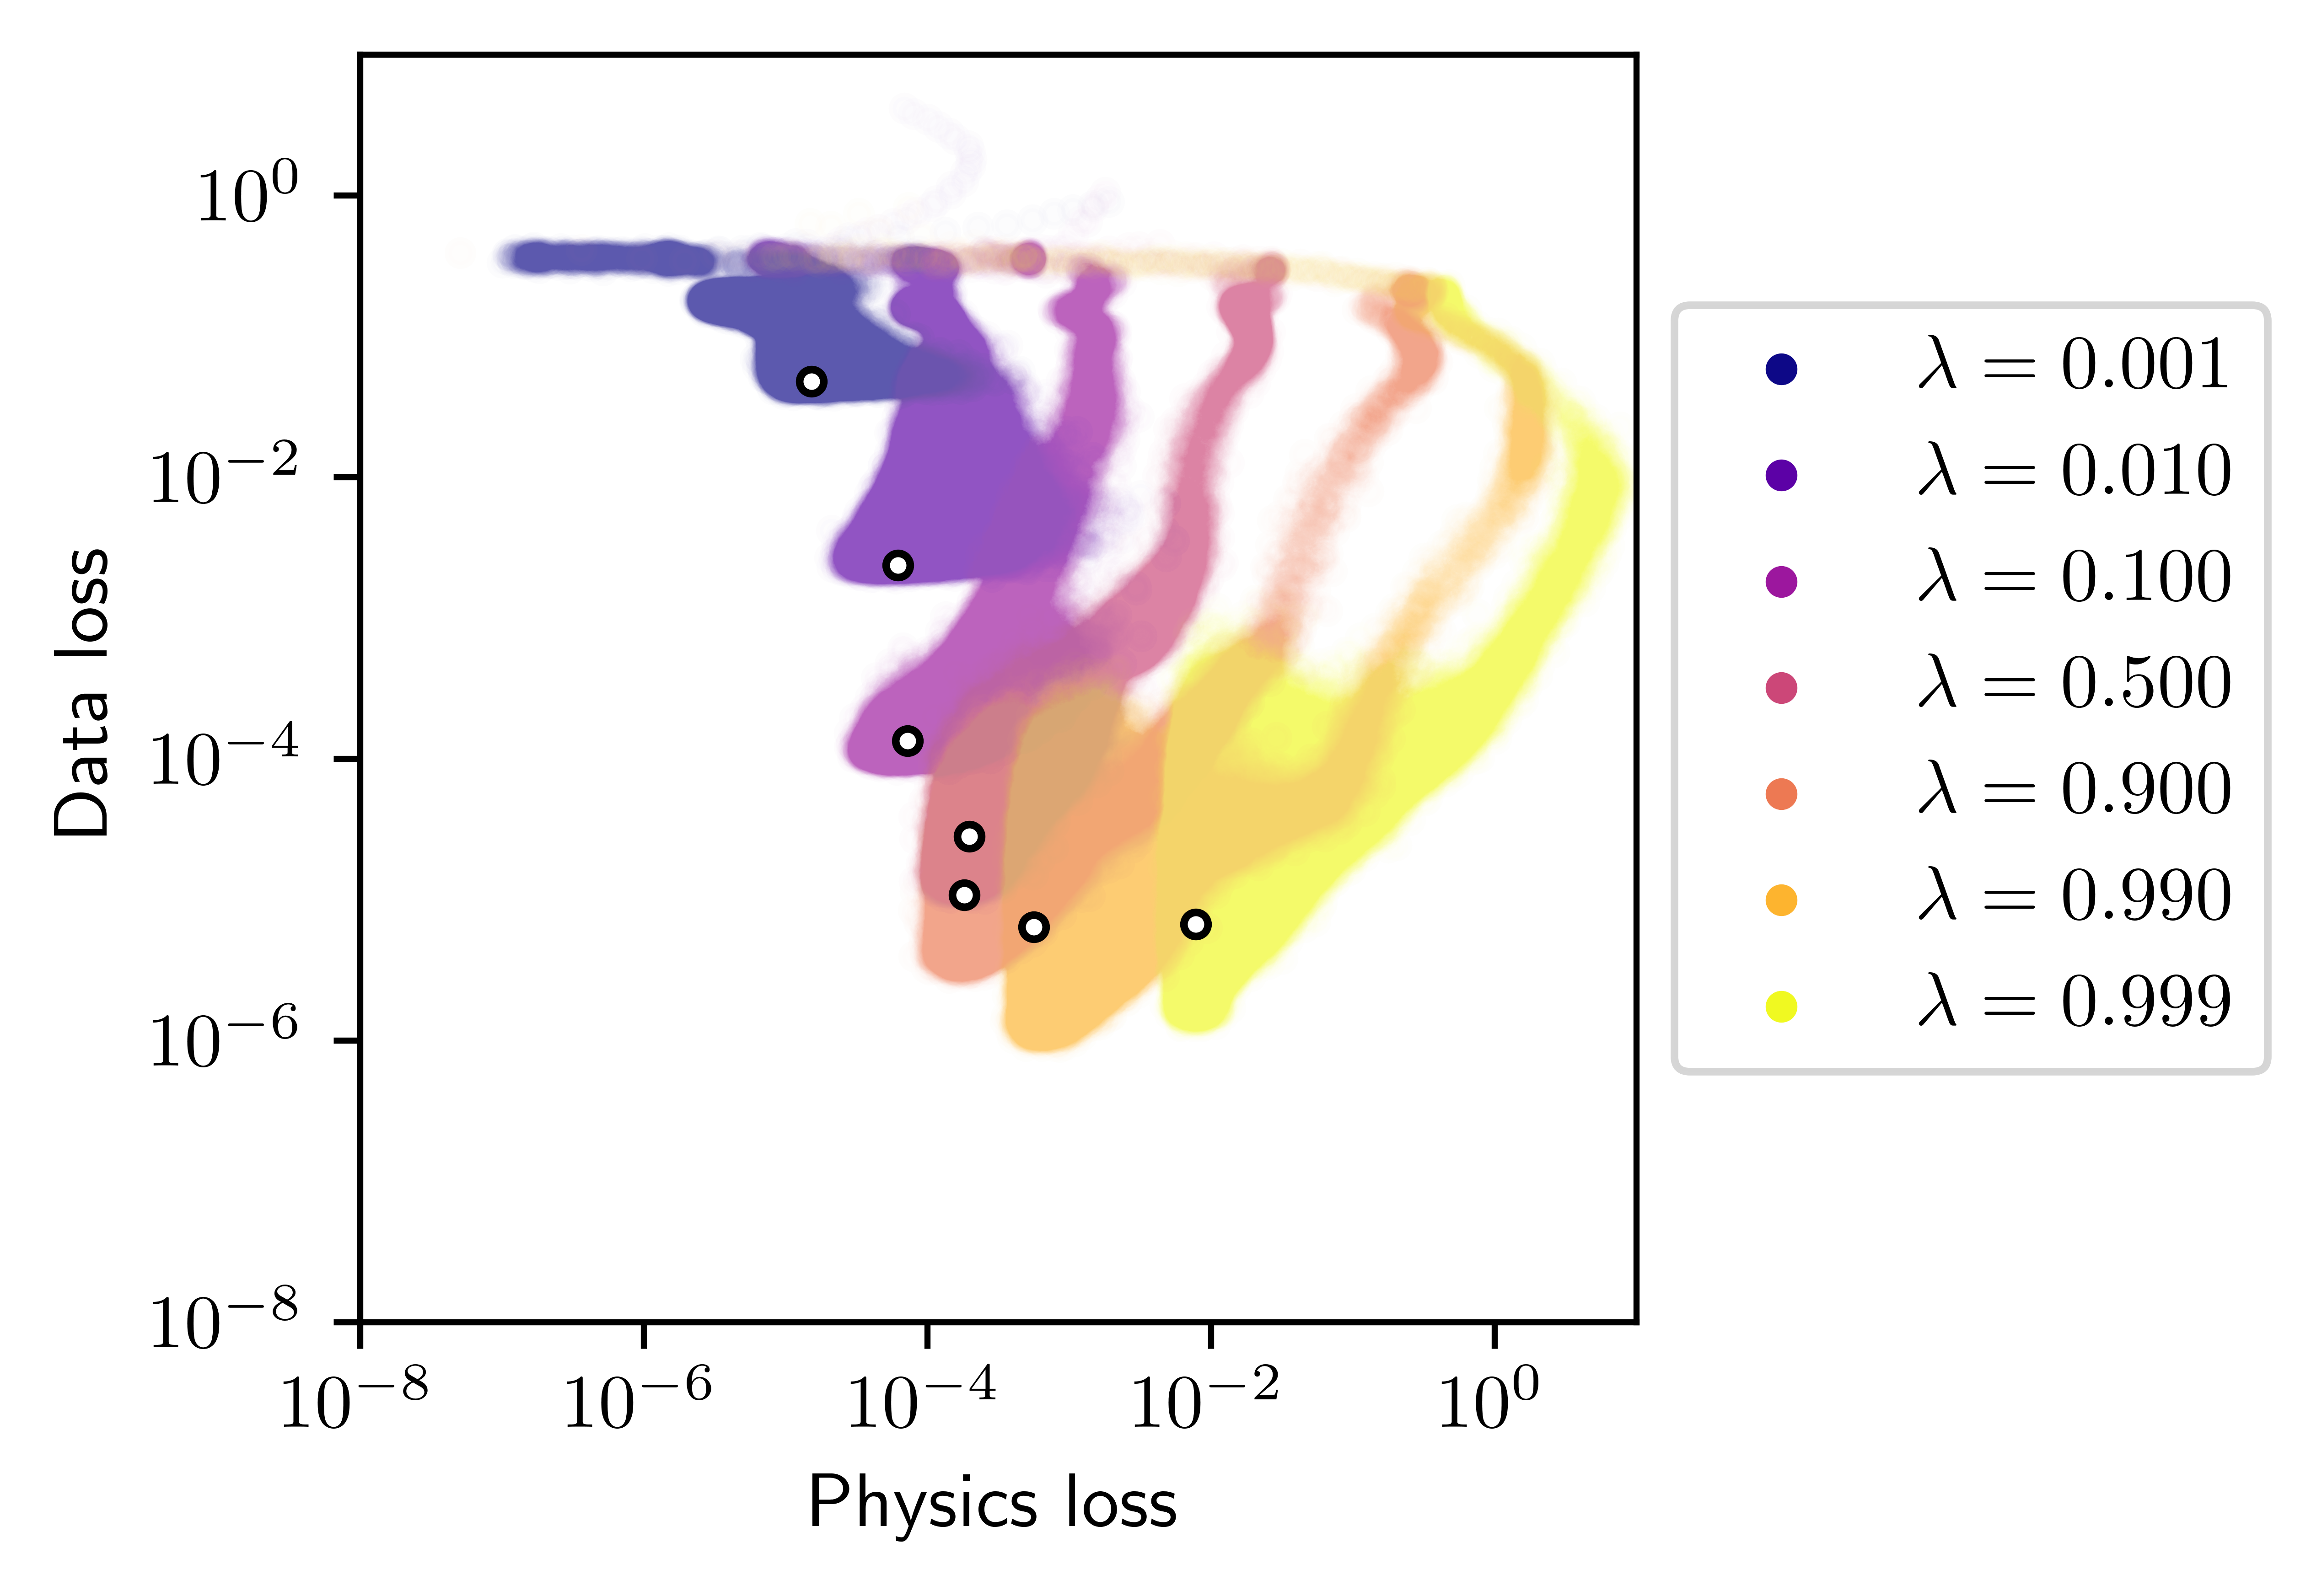
\includegraphics[width=\textwidth]{pareto_front.png}
  \end{minipage}%
  \hfill
  \begin{minipage}{.58\textwidth}
    \begin{itemize}
      \item A Pareto front naturally emerges from the formulation of the problem.
        \par
      \item The \emph{Physics} term is not merely a regularization.
        \par
      \item Need to proceed carefully with the optimization to ensure a physically acceptable solution.
    \end{itemize}
  \end{minipage}
  \vfill
\end{frame}

\begin{frame}
  \vfill
  \centering
  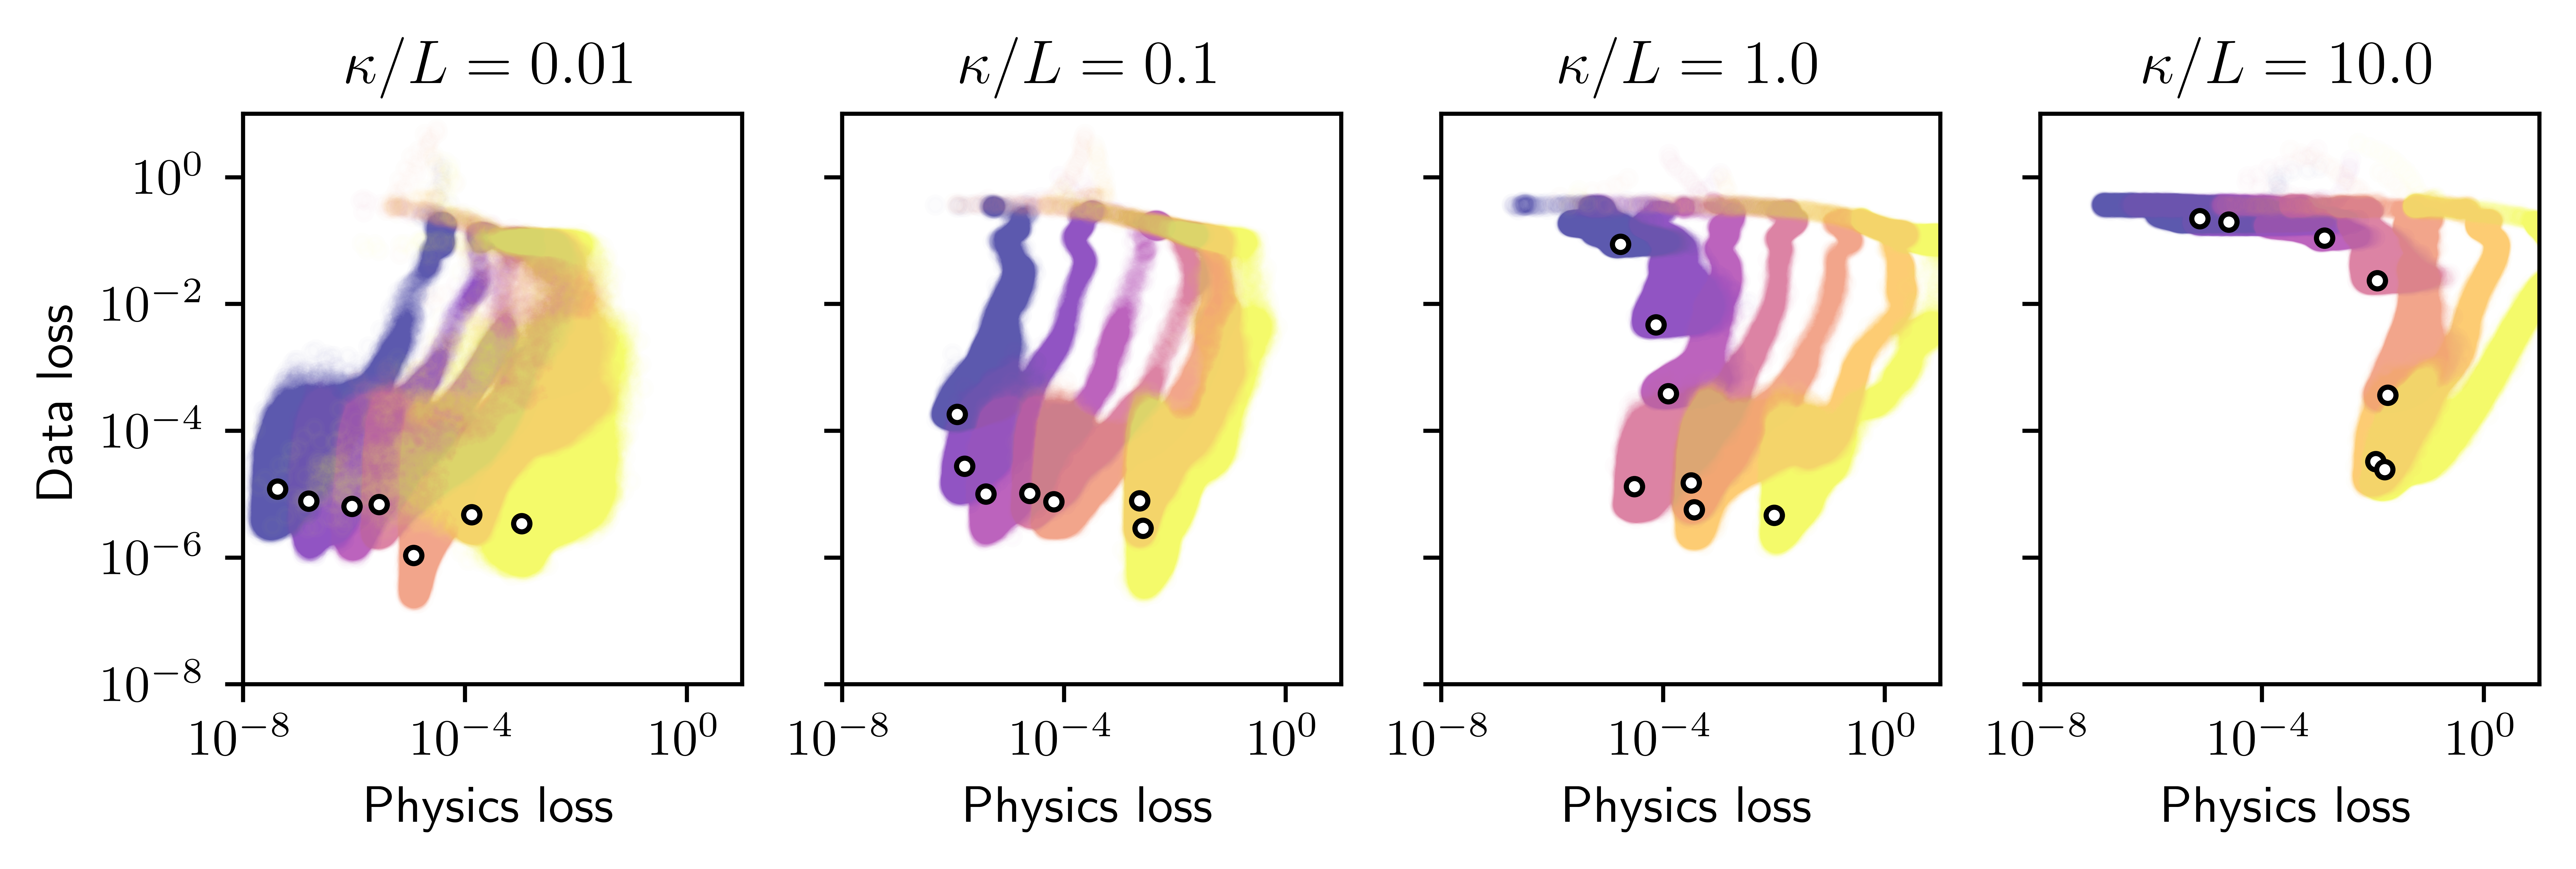
\includegraphics[width=.9\textwidth]{complete_pareto_fronts.png}
  \vfill
\end{frame}

\section{Limitations of PINNs}

\begin{frame}[standout, plain]
  \vfill
  {\usebeamerfont{title} Physics-Informed Neural Nets}

  {\usebeamerfont{subtitle} Limitations}
  \vfill
\end{frame}

\begin{frame}{PDE and optimization}
  \vfill
  \begin{minipage}{.38\textwidth}
    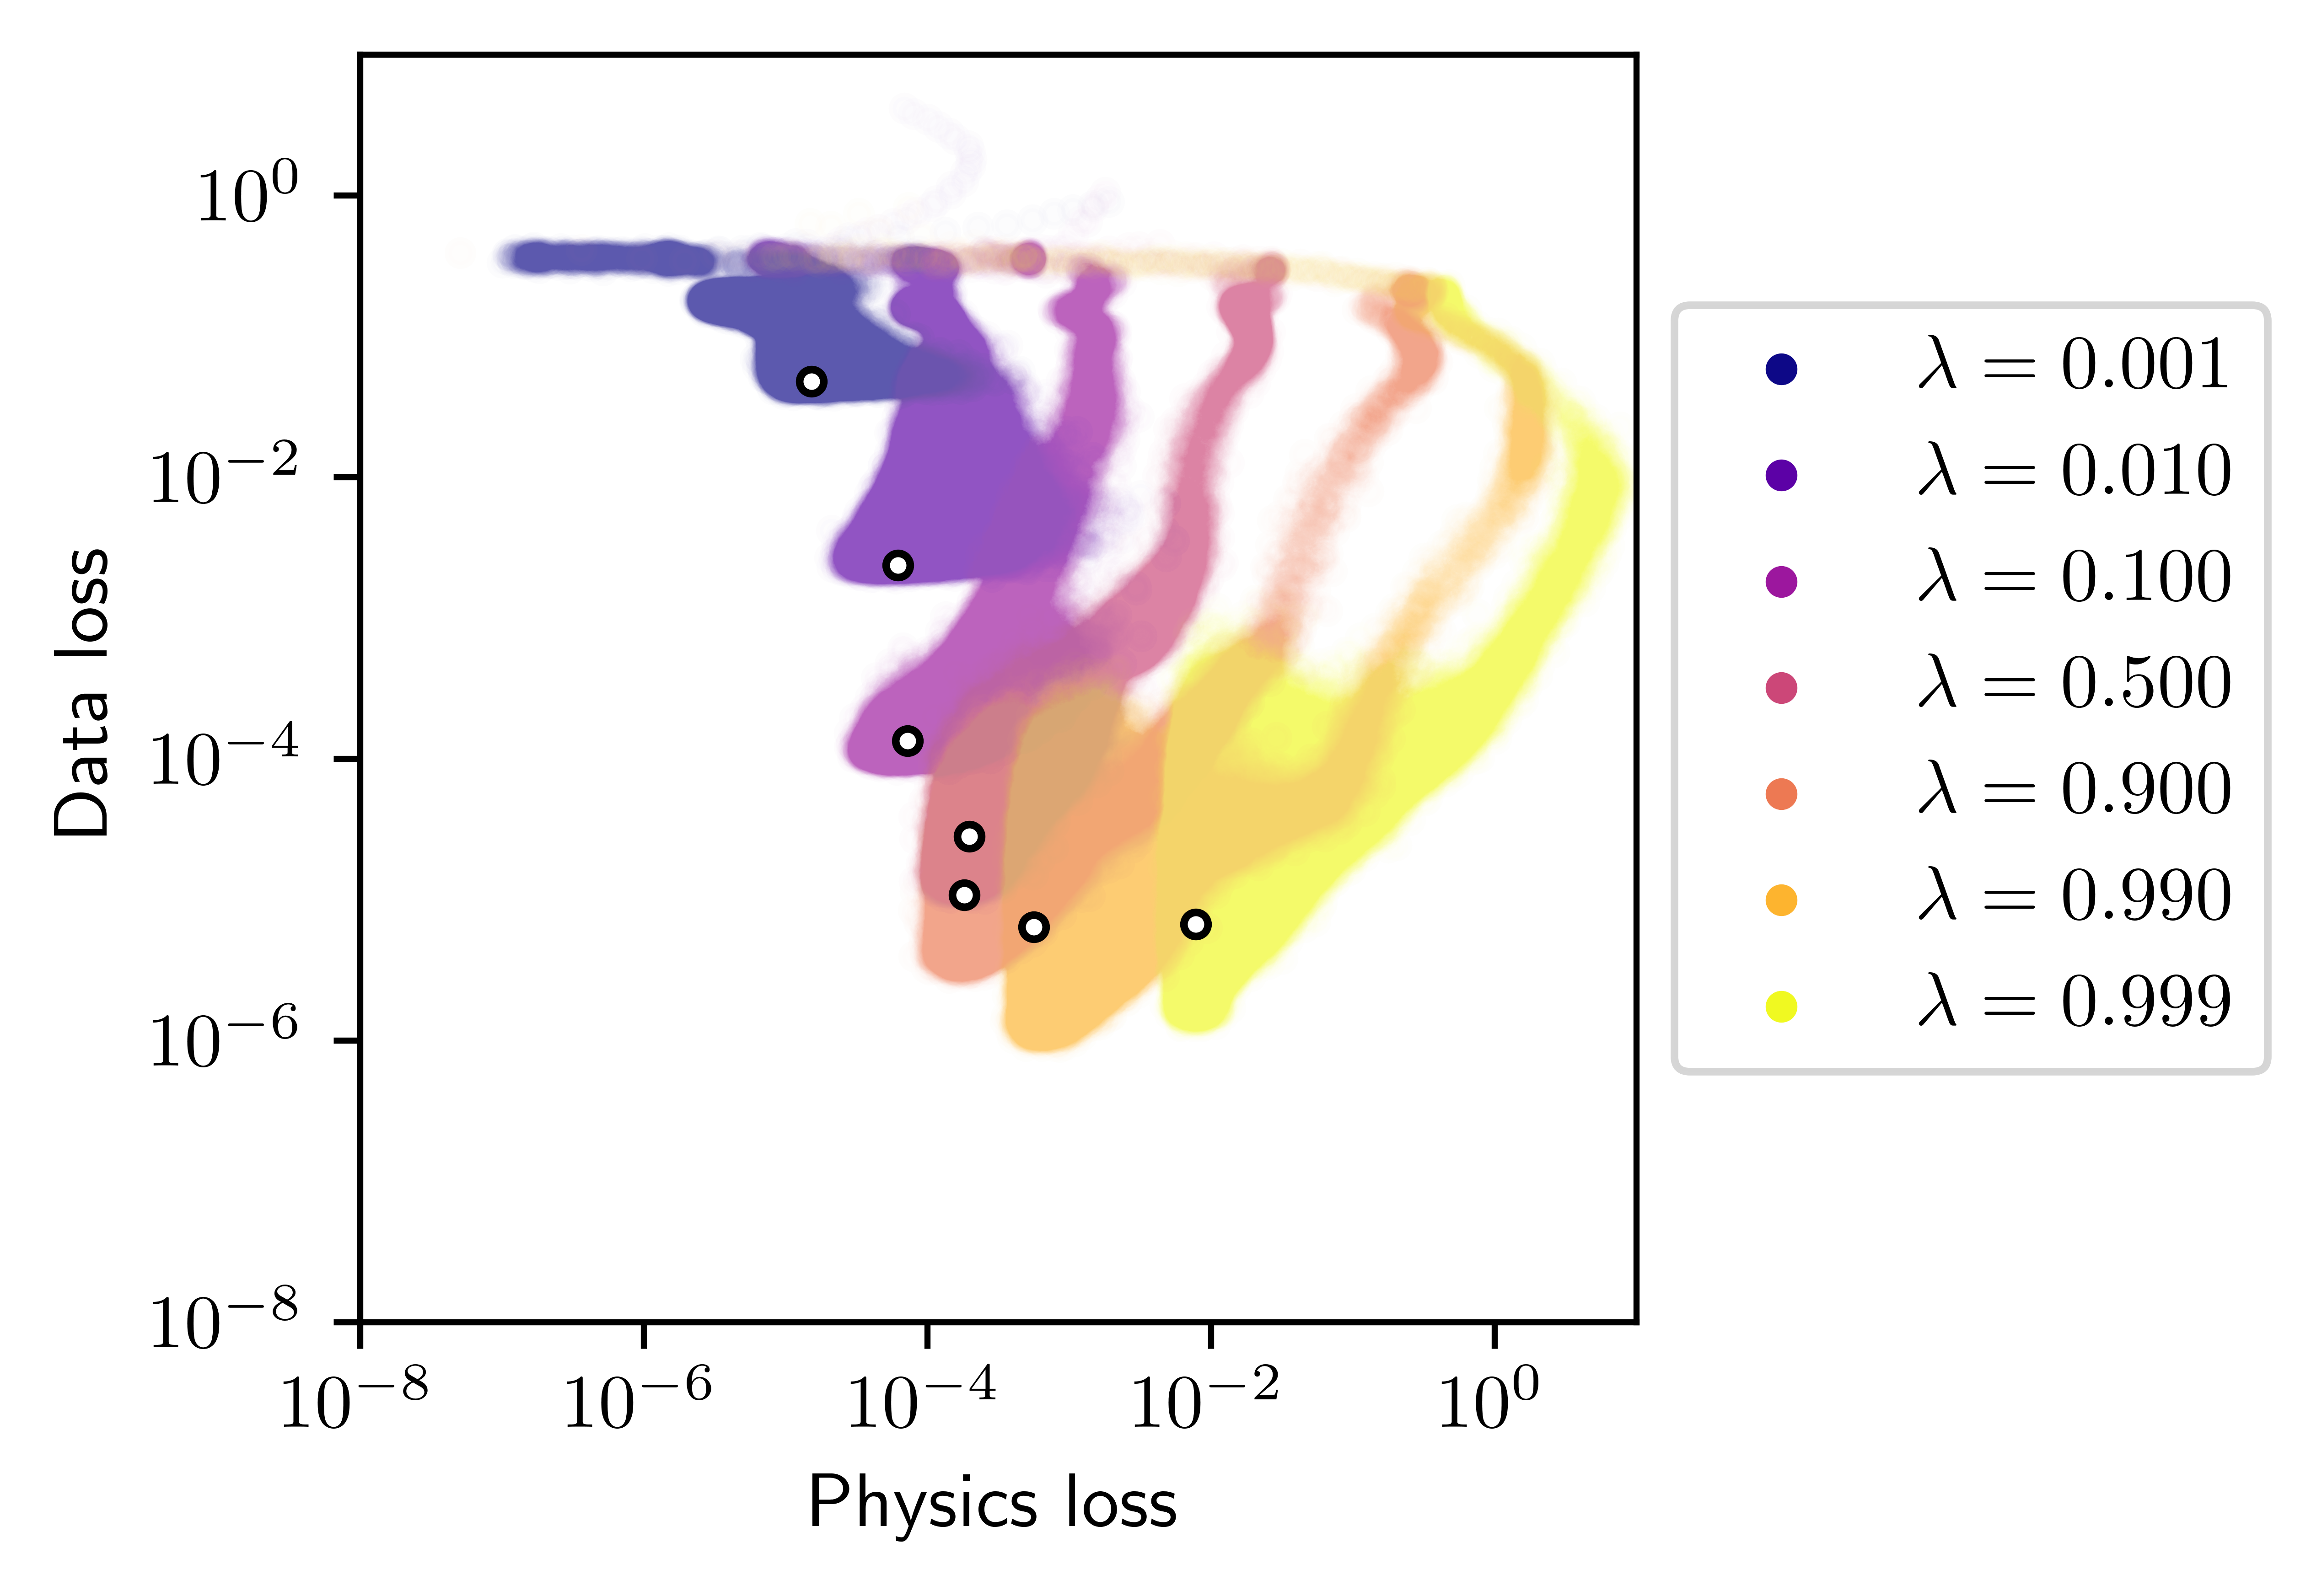
\includegraphics[width=\textwidth]{pareto_front.png}
  \end{minipage}%
  \hfill
  \begin{minipage}{.58\textwidth}
    \centering
    "Solving" an optimization problem
    \[
      \neq
    \]
    Solving a PDE.
  \end{minipage}
  \vfill
\end{frame}

\begin{frame}{Causality}
  \vfill
  \begin{minipage}{.28\textwidth}
    \centering
    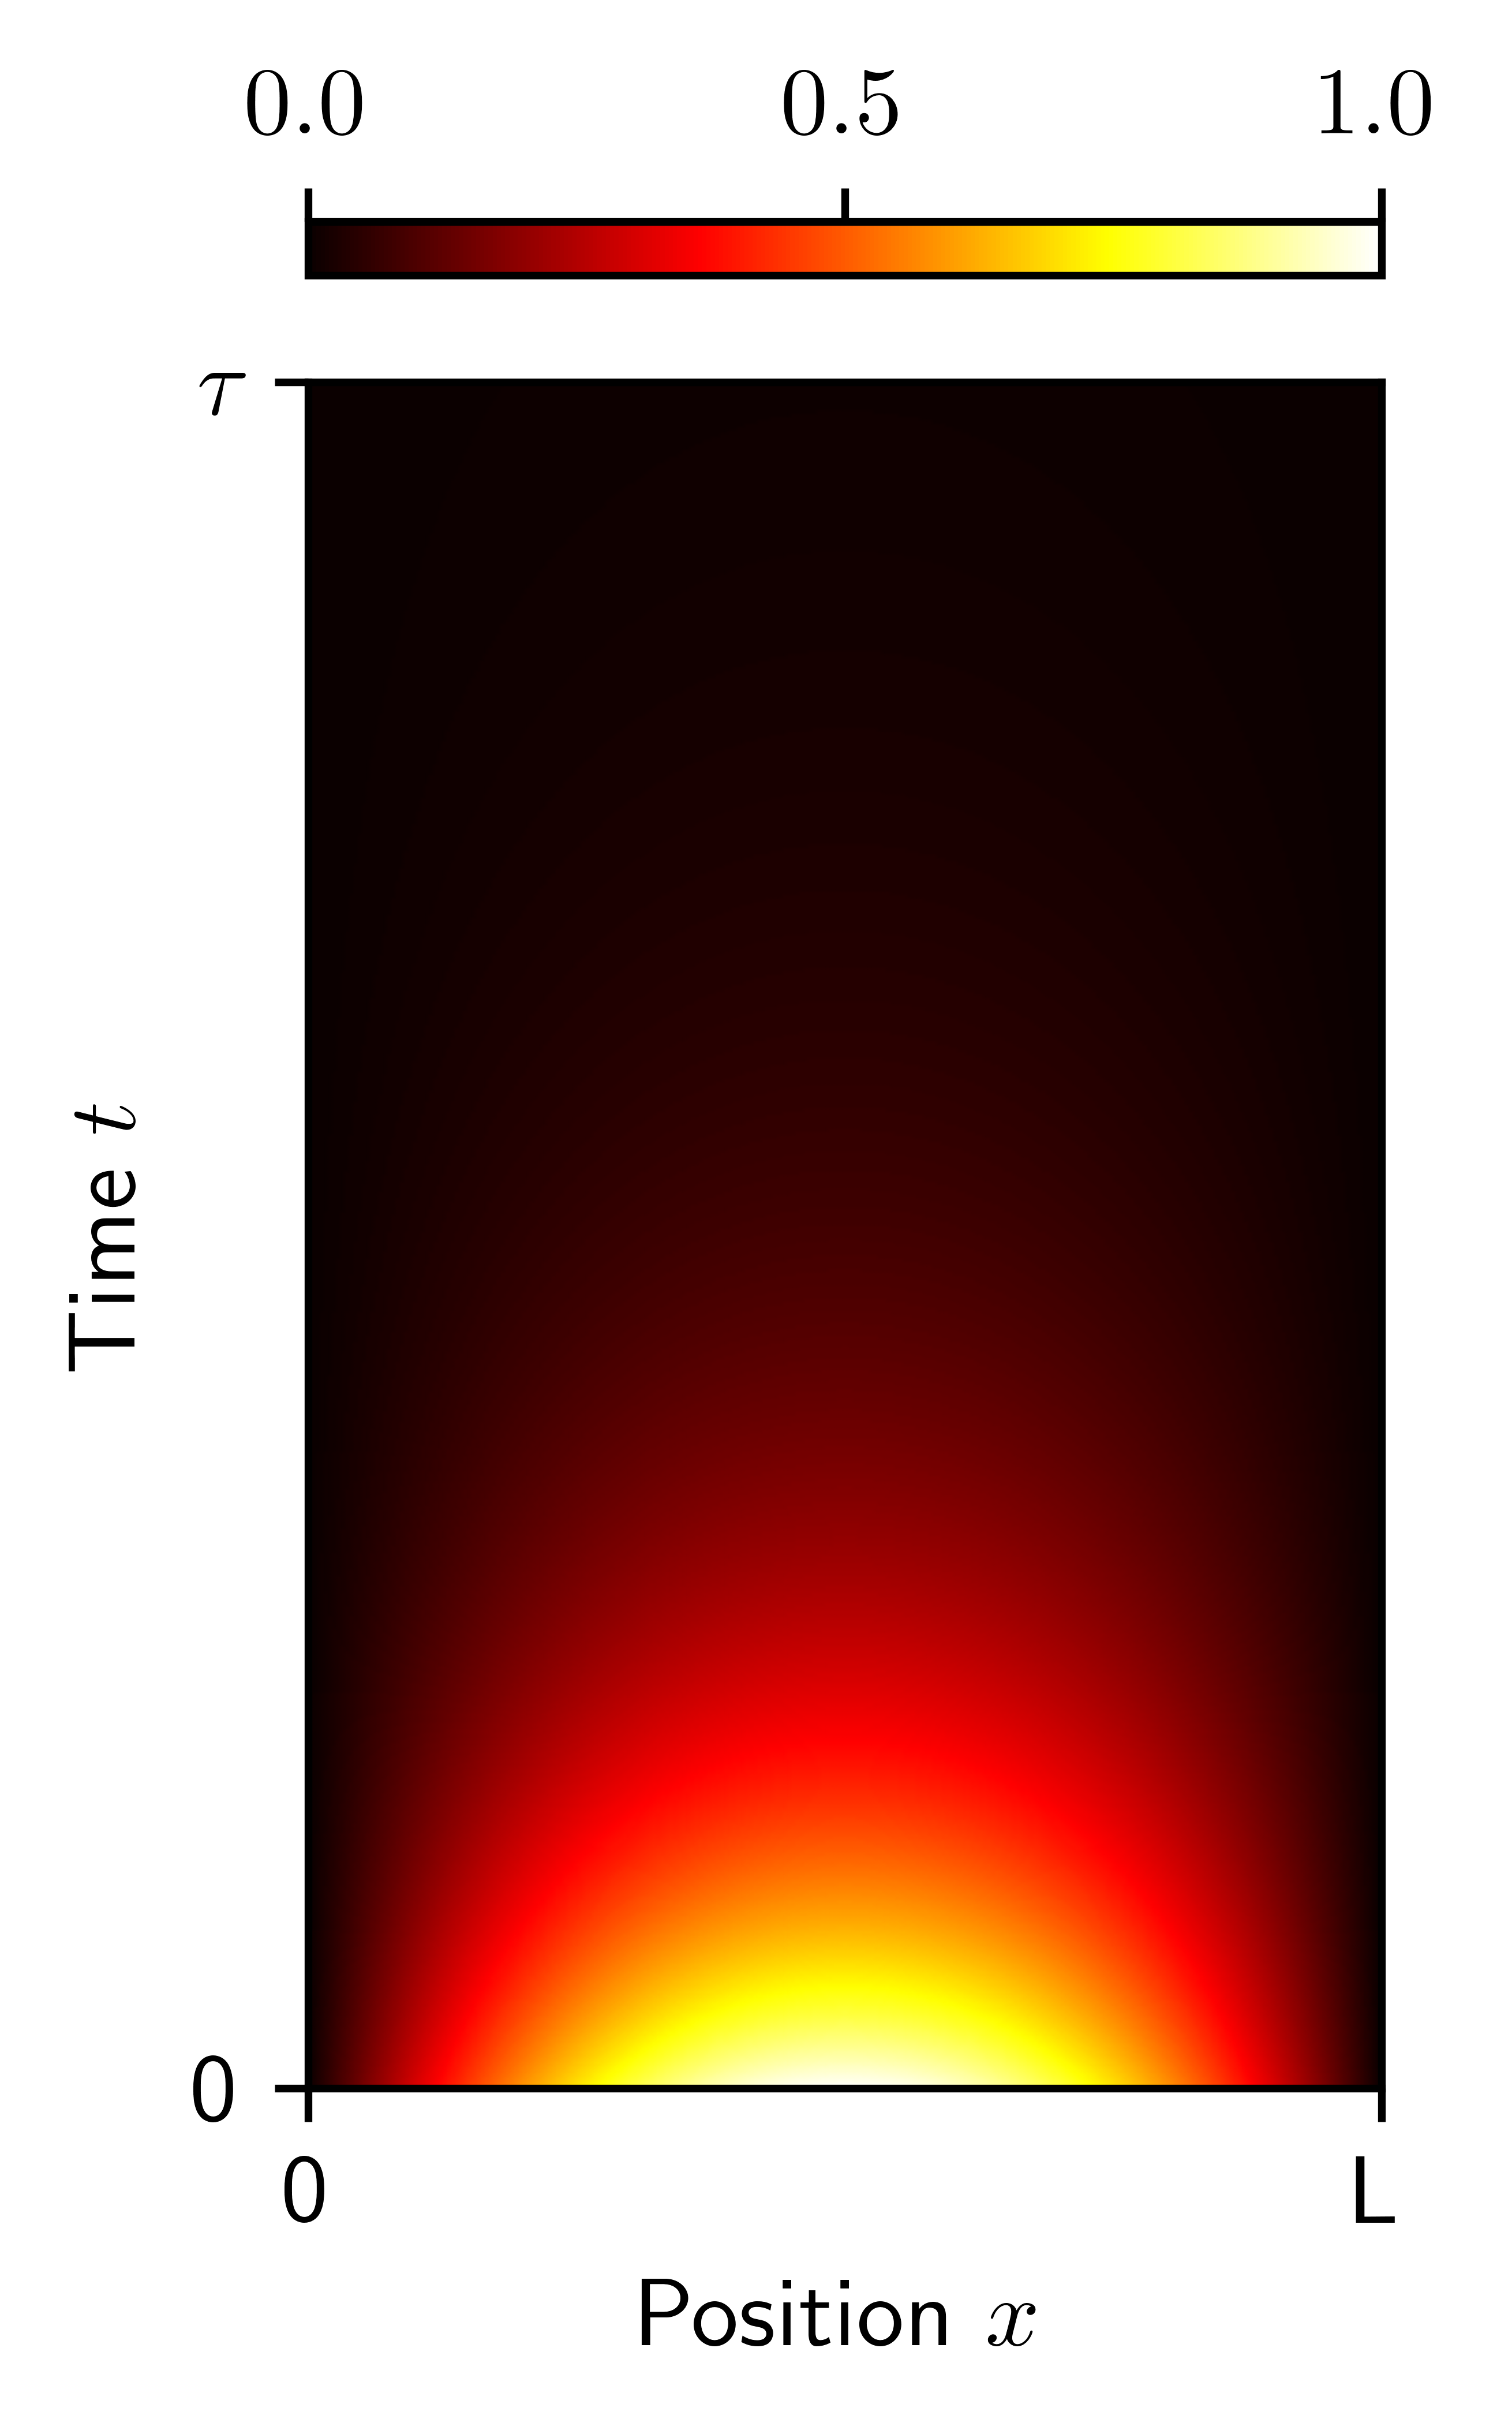
\includegraphics[width=\textwidth]{true_solution.png}
  \end{minipage}%
  \hfill
  \begin{minipage}{.68\textwidth}
  \[
    \left\{
      \begin{aligned}
        & \dfrac{\partial u}{\partial t} = \kappa \dfrac{\partial^2 u}{\partial x^2} \quad \text{for} \quad x \in \left]0, L\right[, \quad  t \in \left[0, T \right]  \\
        & u(0, t) = u(L, t) = 0 \\
        & u(x, 0) = \sin \left( \dfrac{\pi x}{L} \right).
      \end{aligned}
      \right.
    \]
  \end{minipage}
  \vfill
\end{frame}

\begin{frame}{Causality}
  \vfill
  \begin{minipage}{.28\textwidth}
    \centering
    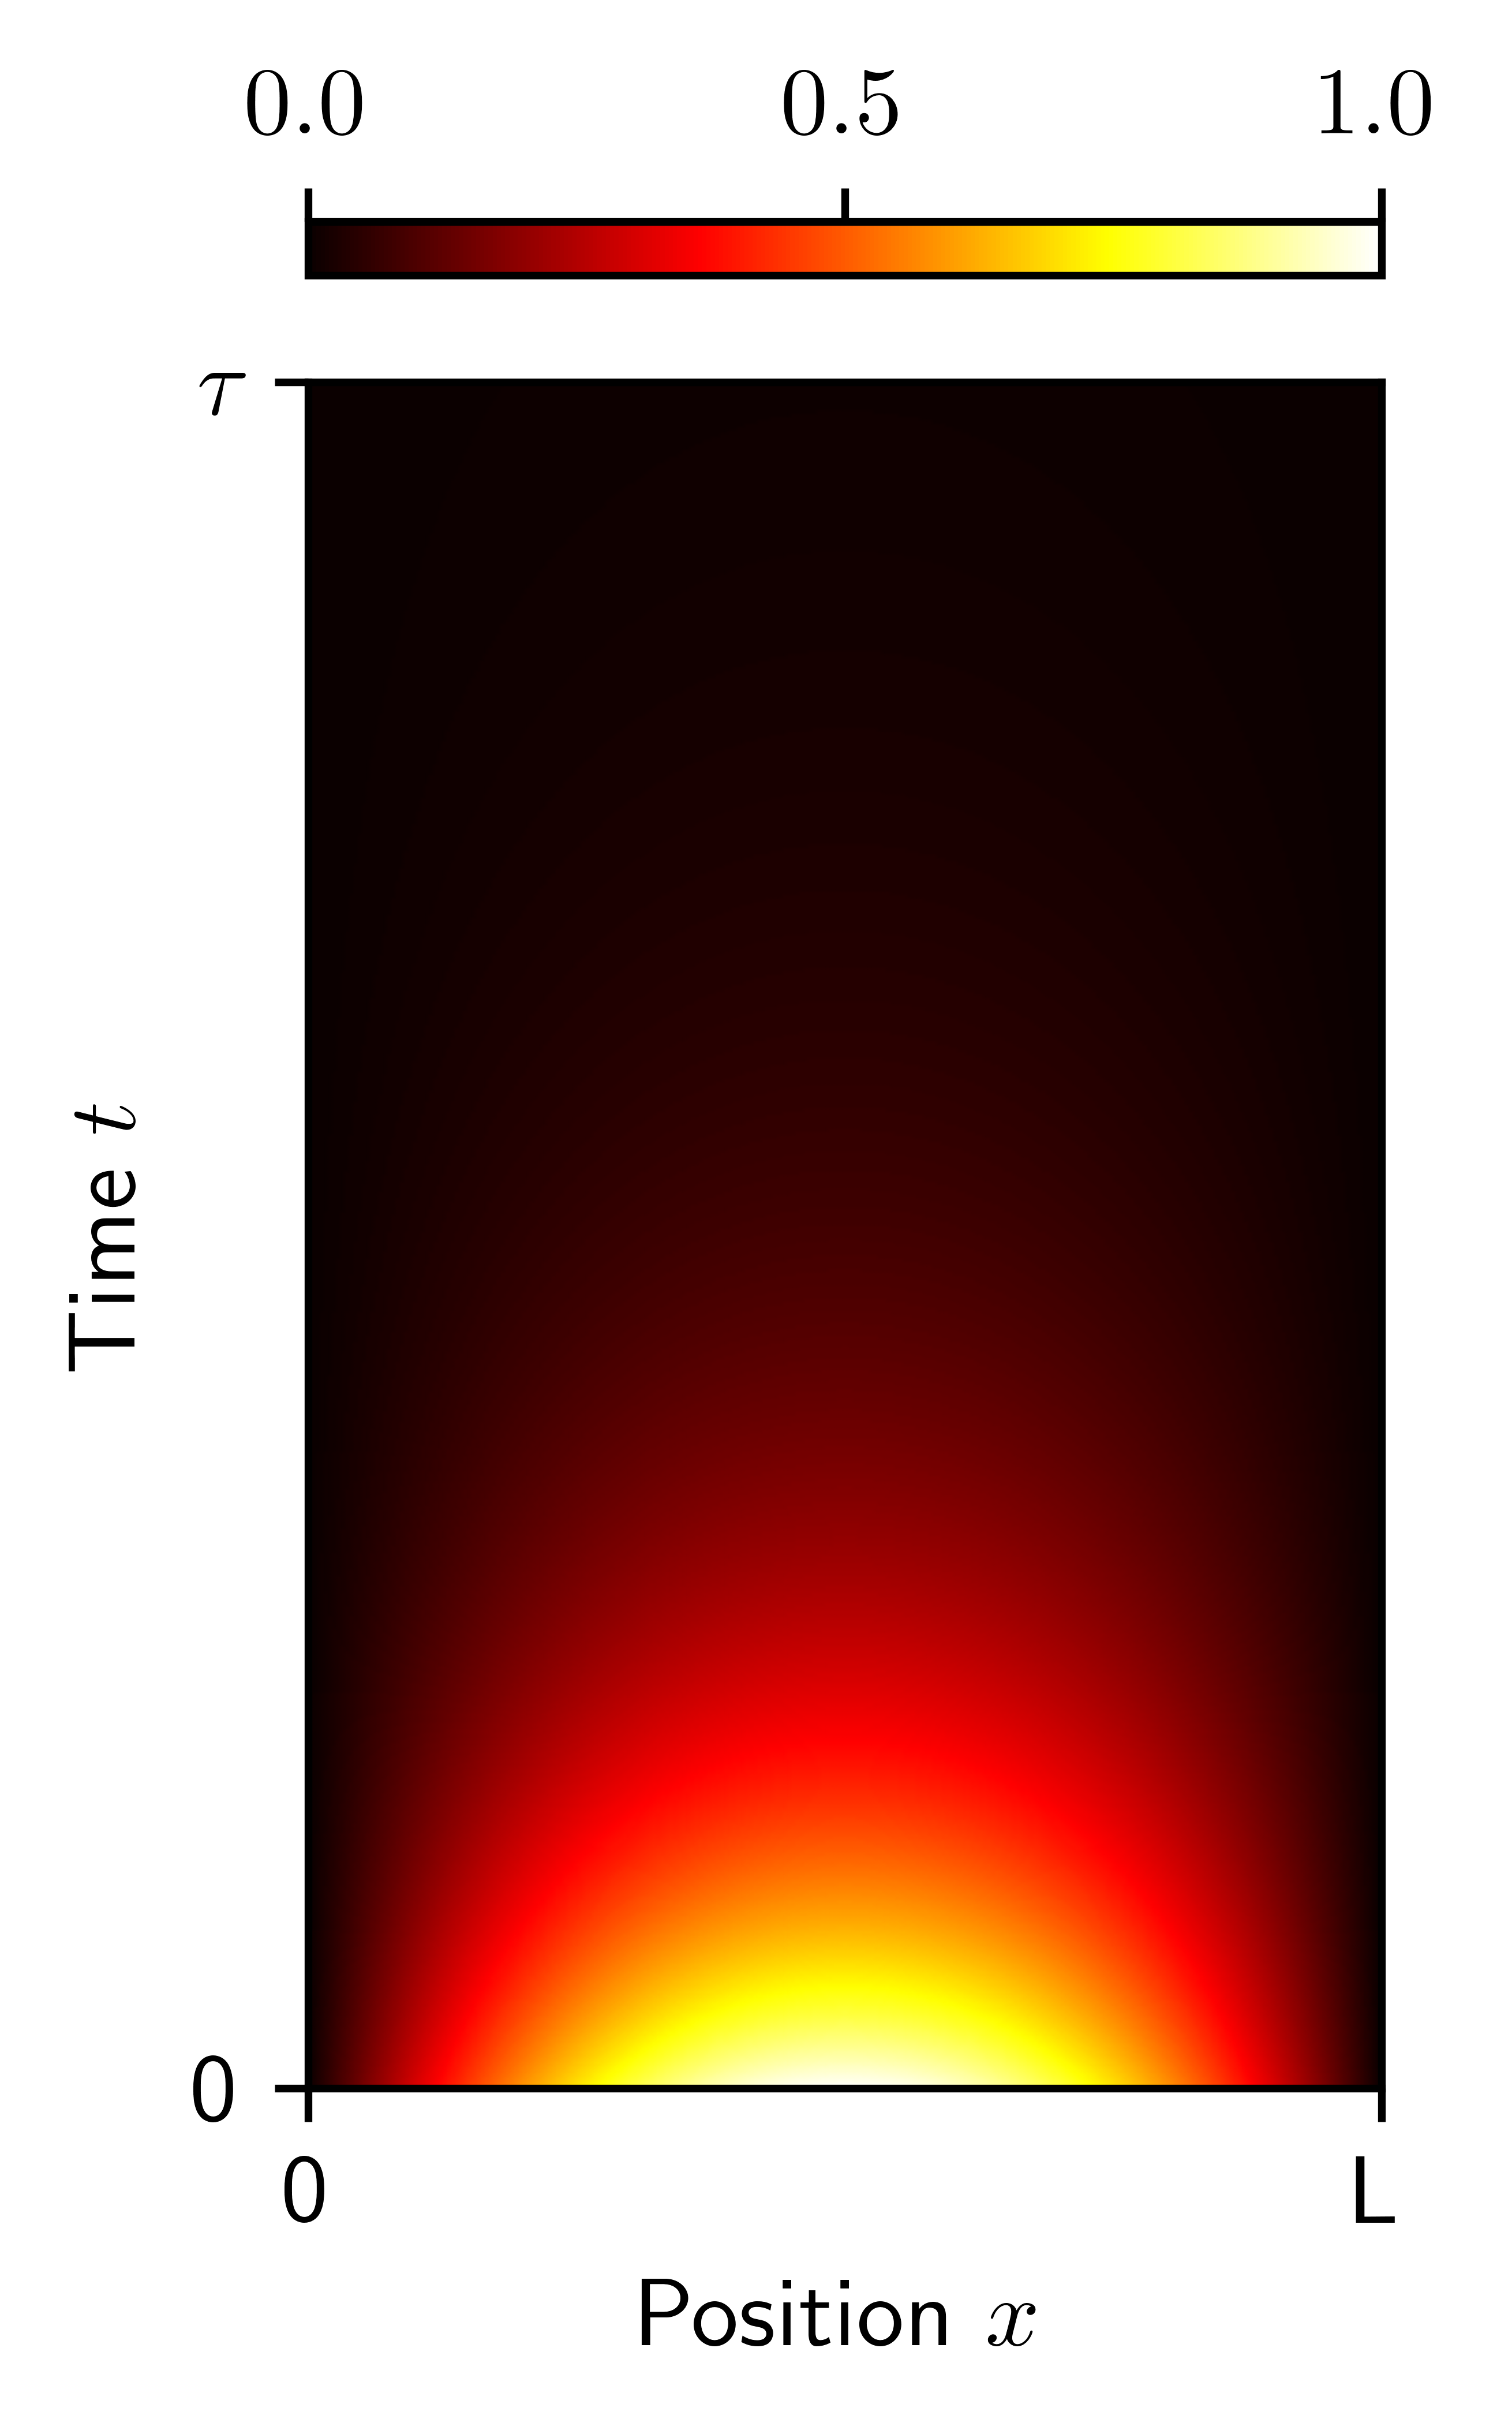
\includegraphics[width=\textwidth]{true_solution.png}
  \end{minipage}%
  \hfill
  \begin{minipage}{.68\textwidth}
    In standard scientific computing, a \emph{time-stepping} approach is used, \ie
    %
    \[
      \vb{u}_{t+1} = f(\vb{u}_t, \vb{u}_{t-1}, \cdots)
    \]
    %
    which naturally enforces the notion of causality.
  \end{minipage}
  \vfill
\end{frame}

\begin{frame}{Causality}
  \vfill
  \begin{minipage}{.28\textwidth}
    \centering
    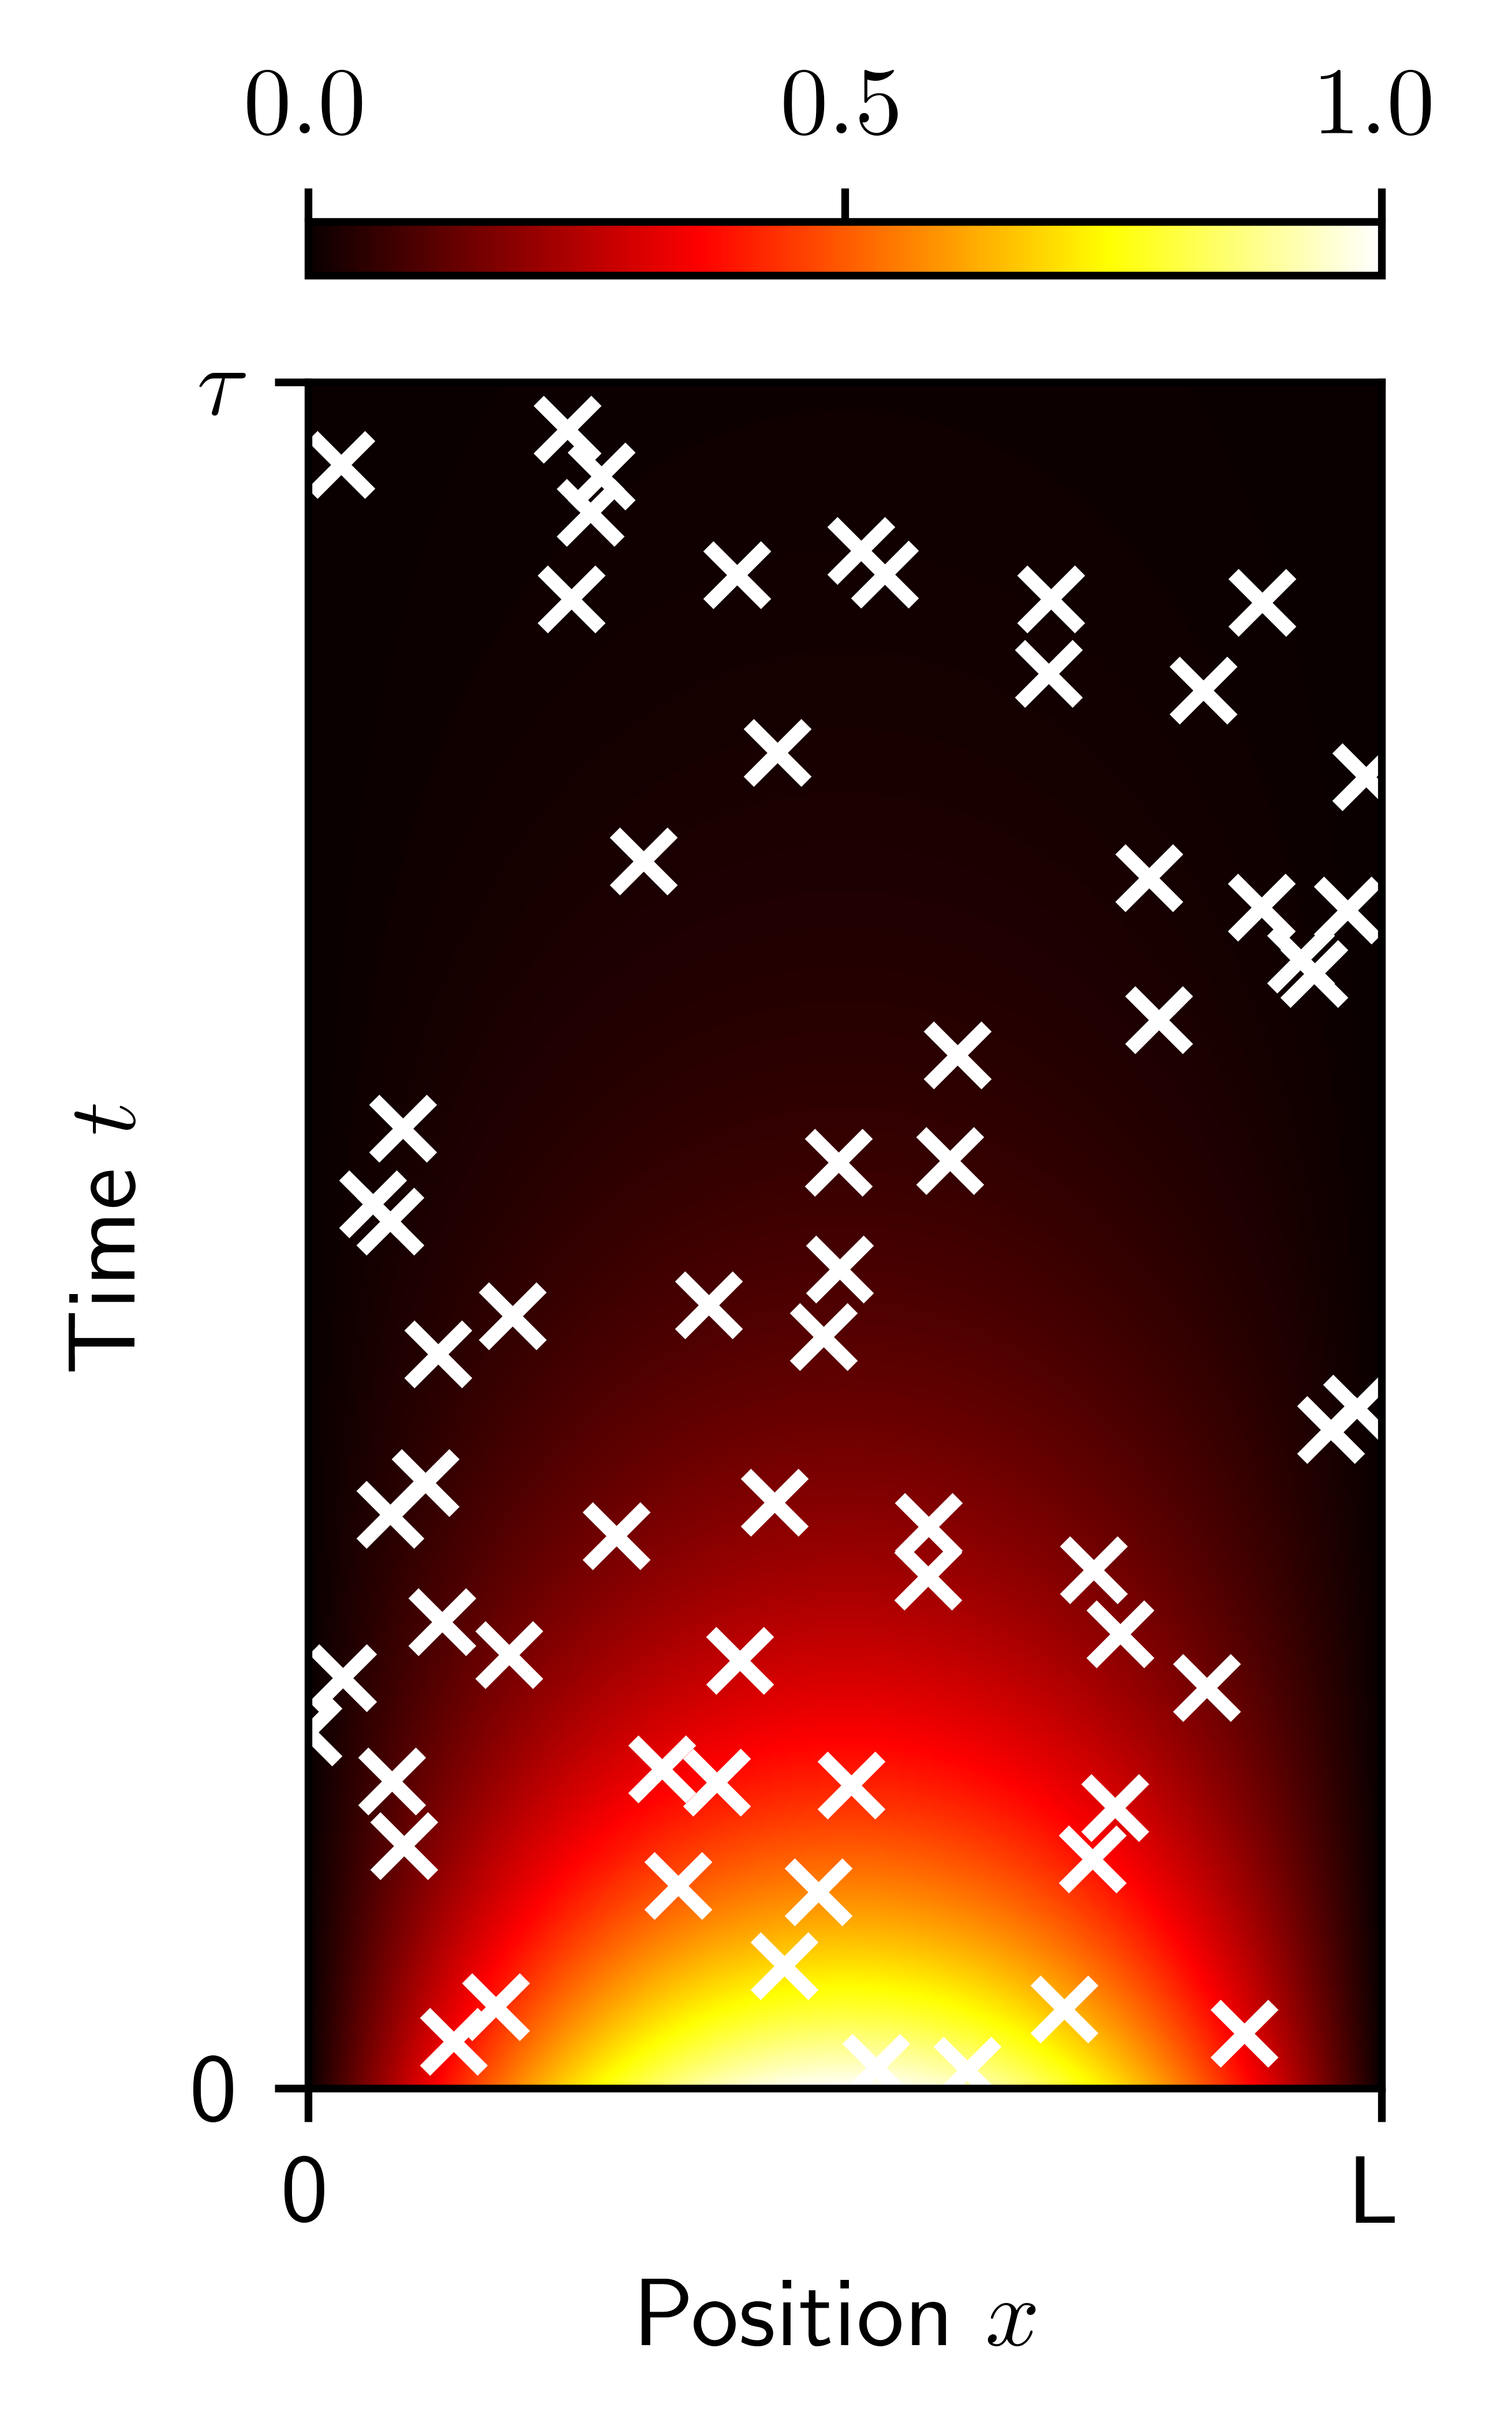
\includegraphics[width=\textwidth]{spatio_temporal_sampling.png}
  \end{minipage}%
  \hfill
  \begin{minipage}{.68\textwidth}
    \[
      \begin{aligned}
        \mathcal{L}_{\varphi}(\boldsymbol{\vartheta}) & = \dfrac{1}{T \cdot L} \int_{0}^{T} \int_{0}^{L} \abs{\mathcal{R}(x, t)}^2 \ \dd x \dd t  \\
          & \simeq \dfrac{1}{N_{\varphi}} \sum_{i=1}^{N_{\varphi}} \abs{ \mathcal{R}(x_i, t_i) }^2
      \end{aligned}
    \]
  \end{minipage}
  \vfill
\end{frame}

\begin{frame}{Causality}
  \vfill
  \begin{minipage}{.28\textwidth}
    \centering
    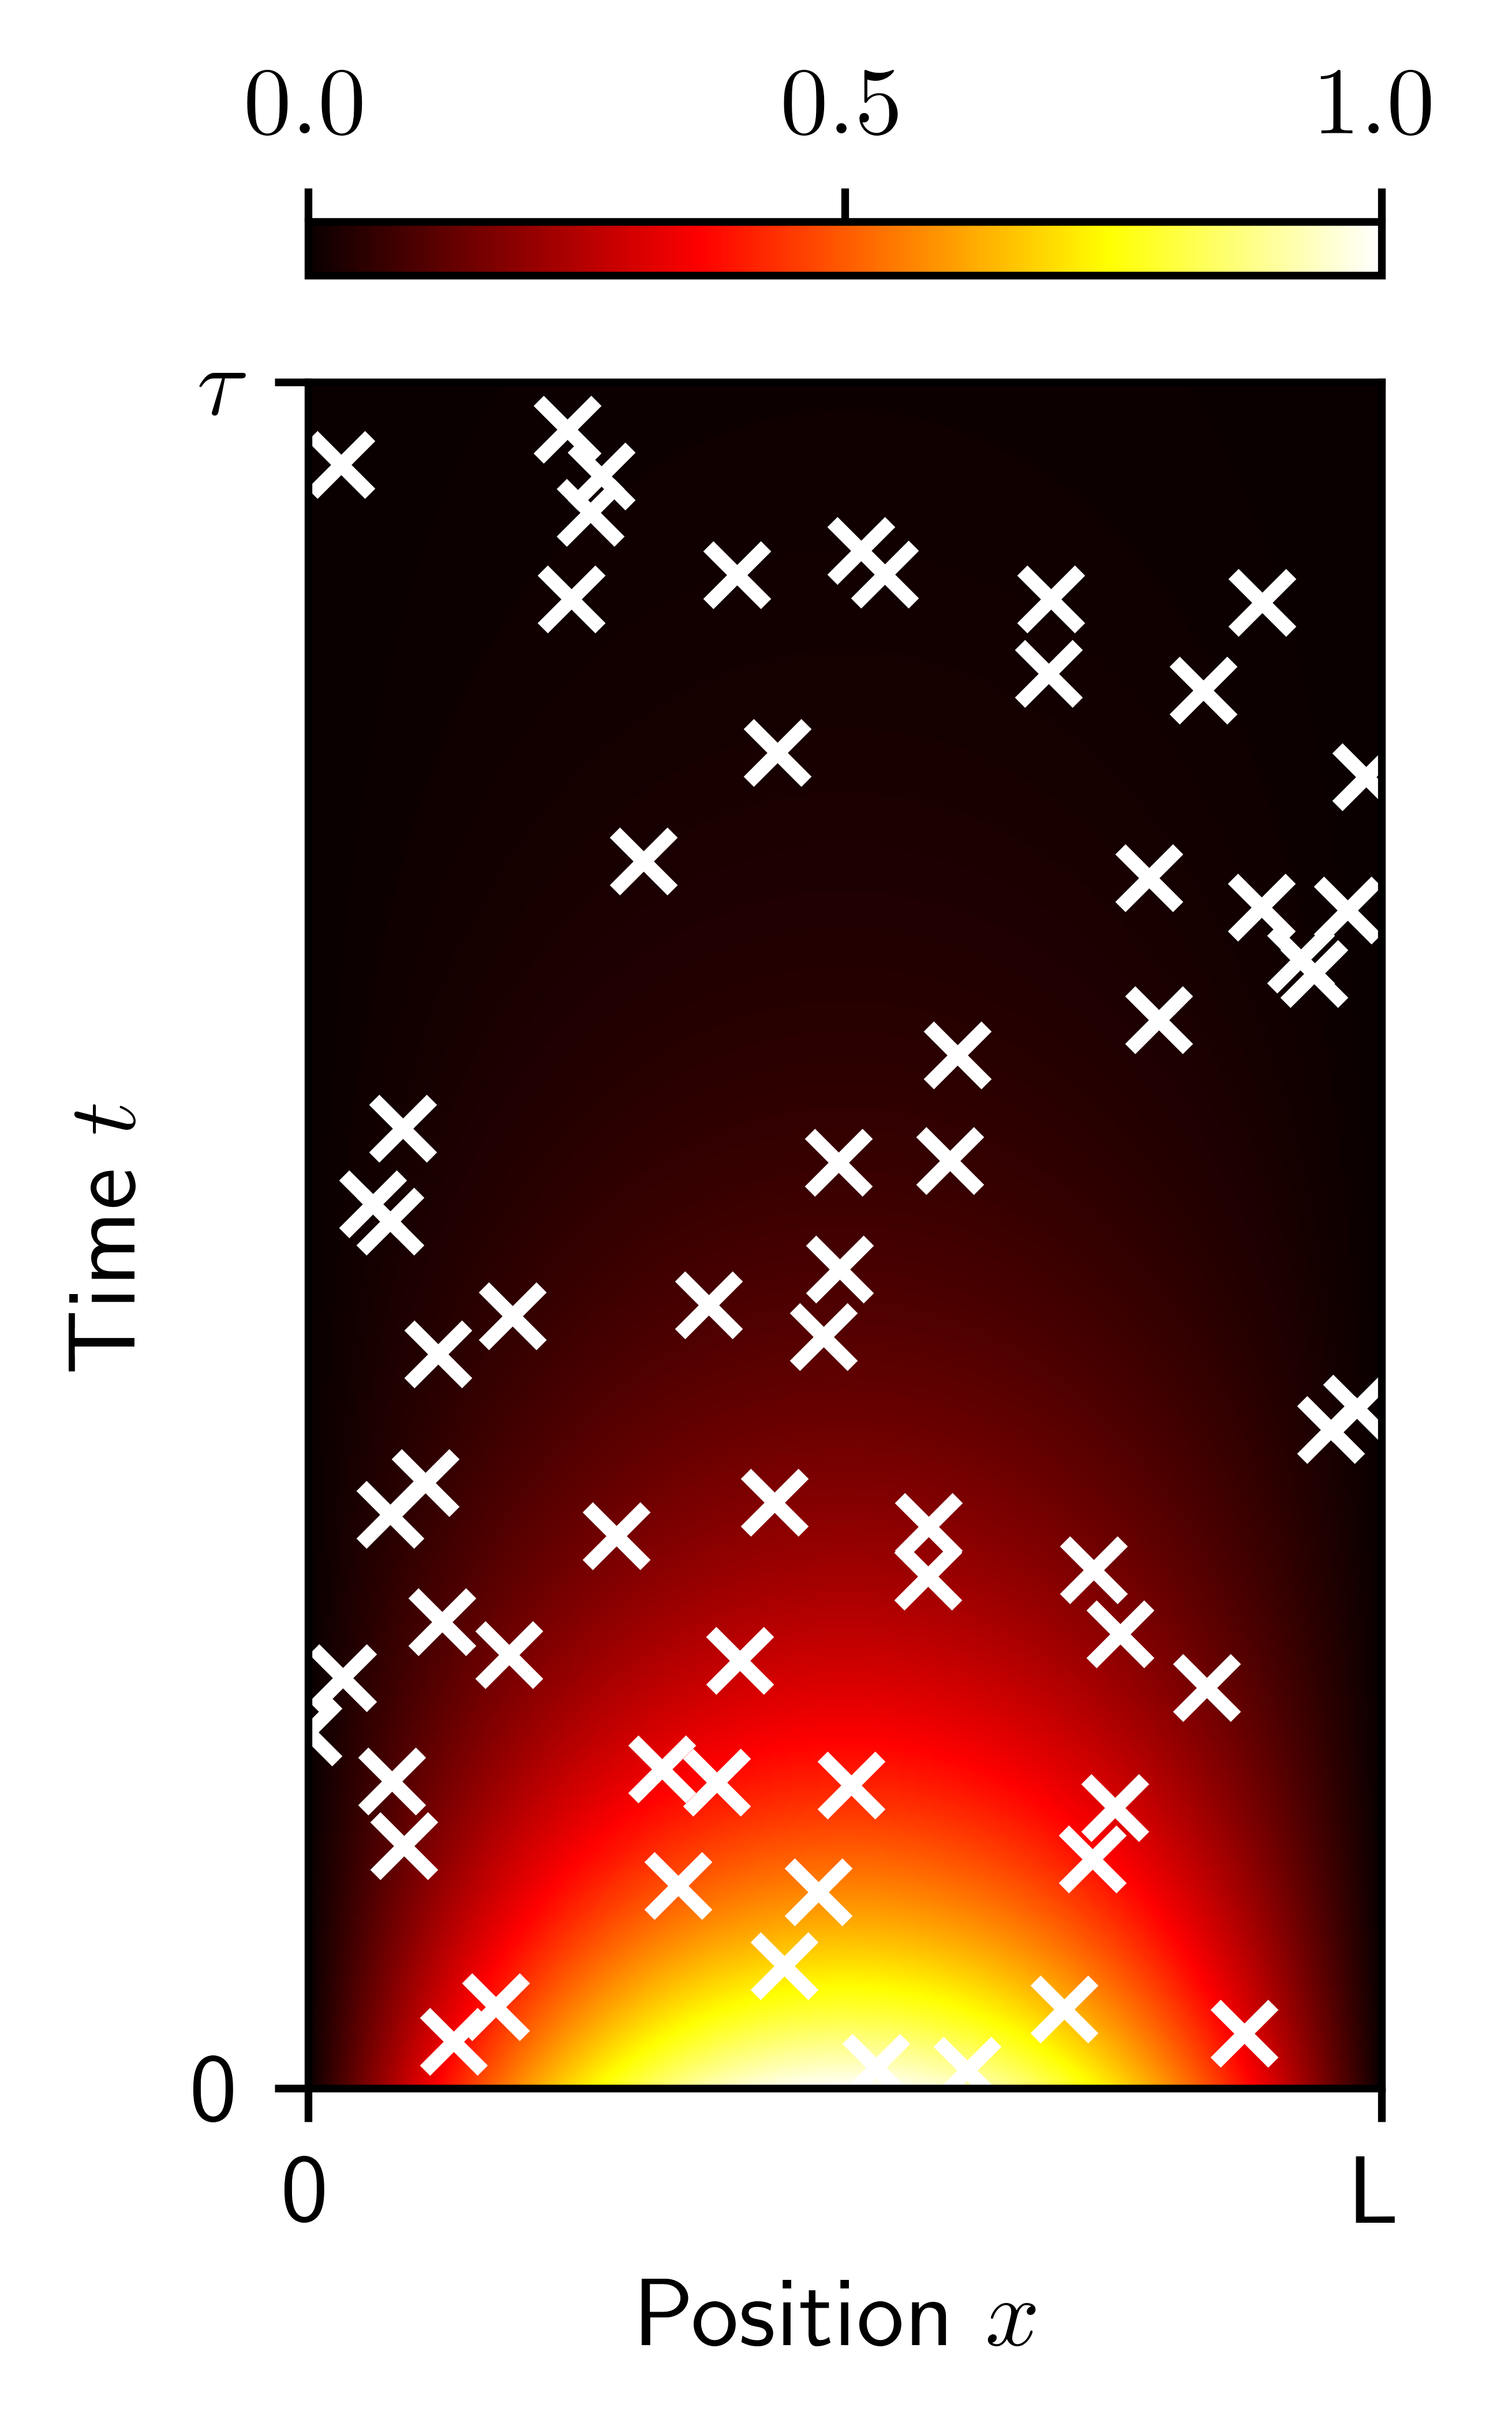
\includegraphics[width=\textwidth]{spatio_temporal_sampling.png}
  \end{minipage}%
  \hfill
  \begin{minipage}{.68\textwidth}
    \[
      \begin{aligned}
        \mathcal{L}_{\varphi}(\boldsymbol{\vartheta}) \simeq \dfrac{1}{N_{\varphi}} \sum_{i=1}^{N_{\varphi}} w_i \abs{ \mathcal{R}(x_i, t_i) }^2
      \end{aligned}
    \]
    %
    with
    %
    \[
      w_i = \exp \left( - \left( \sum_{t_k \leq t_i} \abs{\mathcal{R}(x_k, t_k) }^2 \right) \right)
    \]
  \end{minipage}
  \vfill
\end{frame}

\begin{frame}{Convergence and consistency}
  \vfill
  \vfill
\end{frame}

\begin{frame}{Other limitations}
  \vfill
  \begin{minipage}{.28\textwidth}
    \centering
    \includegraphics[width=\textwidth]{limitation.jpg}
  \end{minipage}%
  \hfill
  \begin{minipage}{.68\textwidth}
    \begin{itemize}
      \item How to ensure conserved quantities are indeed conserved ?
        %
        \[
          \dfrac{\partial \rho}{\partial t} + \nabla \cdot \rho \vb{u} = 0
        \]
        %
      \item How to enforce existing symmetries ?
        %
        \[
          \sigma \cdot \dfrac{\partial u}{\partial t} = f(\sigma \cdot u)
        \]
        %
      \item How to efficiently handle fundamentally multiscale problems ?
    \end{itemize}
  \end{minipage}
  \vfill
\end{frame}

\section{Conclusion}

\begin{frame}[standout, plain]
  \vfill
  {\usebeamerfont{title} Physics-Informed Neural Nets}

  {\usebeamerfont{subtitle} Conclusion}
  \vfill
\end{frame}

\begin{frame}
  \vfill
  \begin{minipage}{.28\textwidth}
    \centering
    
\includegraphics[width=\textwidth]{conclusion.png}
  \end{minipage}%
  \hfill
  \begin{minipage}{.68\textwidth}
    \begin{itemize}
      \item PINNs provide an innovative way to solve ordinary, partial or stochastic differential equations.
        \par
      \item Some theoretical results exist about the convergence of $u_{\vartheta}(x, t)$ to the true solution, but these are scarce.
    \end{itemize}
  \end{minipage}
  \vfill
\end{frame}

\begin{frame}
  \vfill
  \begin{minipage}{.28\textwidth}
    \centering
    
\includegraphics[width=\textwidth]{conclusion.png}
  \end{minipage}%
  \hfill
  \begin{minipage}{.68\textwidth}
    \begin{itemize}
      \item Training a PINN for the sole purpose of simulation can (usually) be a bad idea.
        \begin{itemize}
          \item For "simple" enough problems, scientific computing can go a long way!
        \end{itemize}
        \par
      \item Although not discussed here, PINNs can on the other hand be very advantageous to solve ill-posed inverse problems !
    \end{itemize}
  \end{minipage}
  \vfill
\end{frame}

\begin{frame}{Some open problems}
  \vfill
  \begin{minipage}{.68\textwidth}
    \begin{itemize}
      \item Convergence of the PINN solution to the continuous one beyond elliptic/parabolic equations?
        \par
      \item Rigorous \emph{a priori} error estimates?
        \par
      \item Interplay between PDE type, network architecture, and optimizer.
        \par
      \item etc.
    \end{itemize}
  \end{minipage}%
  \hfill
  \begin{minipage}{.28\textwidth}
    \centering
    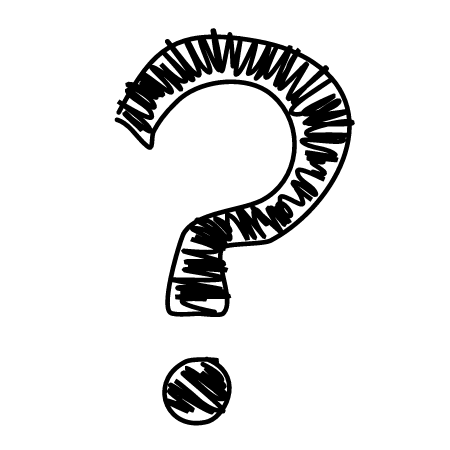
\includegraphics[width=\textwidth]{question.png}
  \end{minipage}
  \vfill
\end{frame}

\begin{frame}{If you want to know more}
  \vfill
  \begin{minipage}{.28\textwidth}
    \centering
    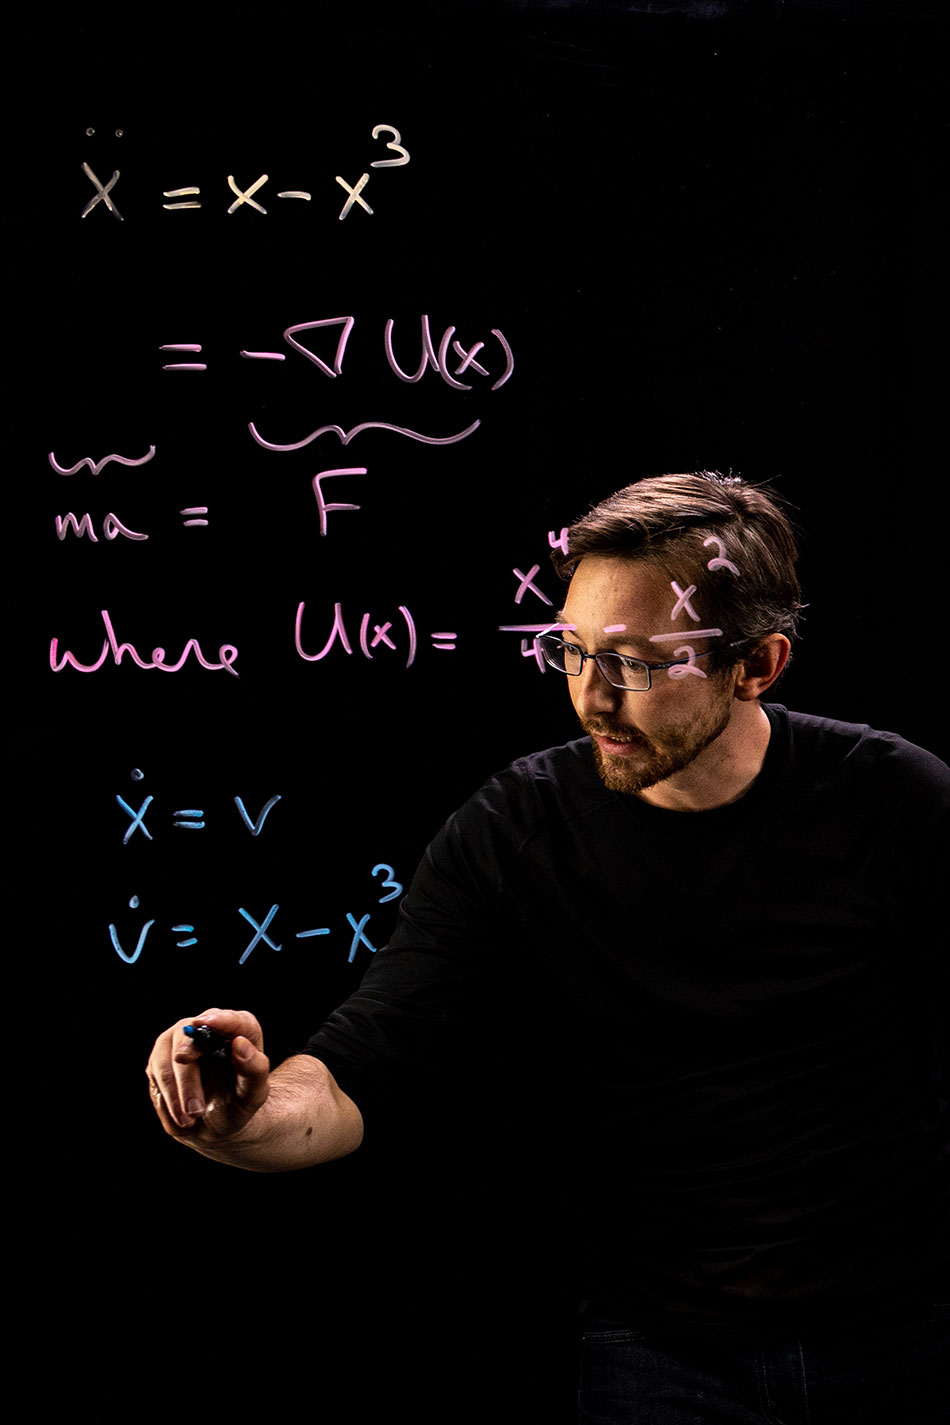
\includegraphics[width=\textwidth]{steve.jpg}
  \end{minipage}%
  \hfill
  \begin{minipage}{.68\textwidth}
    Steve Brunton (UW, Seattle) has some very good educational resources:
    %
    \par\medskip
    %
    \begin{itemize}
      \item[\faYoutube] \url{youtube.com/@Eigensteve}
      \item[\faBook]  \emph{Data-driven Science and Engineering}, Cambridge Uni. Press.
    \end{itemize}
    %
    \par\medskip
    %
    Many other resources can be found online! Be curious!
  \end{minipage}
  \vfill
\end{frame}

\End

\begin{frame}[plain,standout]
    \vfill
    \begin{minipage}{.68\textwidth}
        {
            \Large
            \textbf{Thank you for your attention!}
        }
        \par\bigskip
        {
            Any questions?
        }
    \end{minipage}%
    \hfill
    \begin{minipage}{.28\textwidth}
        \centering
        \scalebox{4}{\faGithub} \par\bigskip
        \tiny
        \url{loiseaujc.github.io}
    \end{minipage}
    \vfill
\end{frame}

\end{document}
